\documentclass{report}
\usepackage{setspace}
%\usepackage{subfigure}

\pagestyle{plain}
\usepackage{amssymb,graphicx,color}
\usepackage{amsfonts}
\usepackage{latexsym}
\usepackage{a4wide}
\usepackage{amsmath}
\usepackage{enumitem}
\usepackage{booktabs}

\newtheorem{theorem}{THEOREM}
\newtheorem{lemma}[theorem]{LEMMA}
\newtheorem{corollary}[theorem]{COROLLARY}
\newtheorem{proposition}[theorem]{PROPOSITION}
\newtheorem{remark}[theorem]{REMARK}
\newtheorem{definition}[theorem]{DEFINITION}
\newtheorem{fact}[theorem]{FACT}

\newtheorem{problem}[theorem]{PROBLEM}
\newtheorem{exercise}[theorem]{EXERCISE}
\def \set#1{\{#1\} }

\newenvironment{proof}{
PROOF:
\begin{quotation}}{
$\Box$ \end{quotation}}



\newcommand{\nats}{\mbox{\( \mathbb N \)}}
\newcommand{\rat}{\mbox{\(\mathbb Q\)}}
\newcommand{\rats}{\mbox{\(\mathbb Q\)}}
\newcommand{\reals}{\mbox{\(\mathbb R\)}}
\newcommand{\ints}{\mbox{\(\mathbb Z\)}}

% Generated result macros from the checksum-verified 60 Hz v5 formal cohort.
% Loaded here, not inside Chapter 6, so that Chapter 7 and the abstract quote
% the same frozen values instead of restating them by hand.
\input{experiment_results/reanalysis_rescue_60_v5/chapter6_numbers.tex}

% hyperref must be loaded last. Provides \url in the source-code appendix.
\usepackage[hidelinks]{hyperref}

%%%%%%%%%%%%%%%%%%%%%%%%%%


\title{  	{ 
\includegraphics[scale=.5]{ucl_logo.png}}\\
{{\Huge A Real-Time Music-Conditioned Framework for Motion Retrieval, Retargeting, and Adaptive Humanoid Control}}
		}
\date{Submission date: 07/08/2026}
\author{Chengjun Ouyang\thanks{
{\bf Disclaimer:}
This report is submitted as part requirement for the MSc Machine Learning at UCL. It is
substantially the result of my own work except where explicitly indicated in the text.
 The report may be freely copied and distributed provided the source is explicitly acknowledged
}
\\ \\
MSc Machine Learning\\ \\
Supervisor: Prof Chengxu Zhou}



\begin{document}
 
 \onehalfspacing
\hypersetup{pageanchor=false}
\maketitle
% Front matter is numbered in roman so that Chapter 1 can start at arabic page 1
% without reusing numbers already spent on the title, abstract and contents.
% Page anchors are off here so hyperref does not emit duplicate page.1 targets.
\hypersetup{pageanchor=false}
\pagenumbering{roman}
\begin{abstract}


Live music-driven humanoid dance requires musical relevance, responsive timing,
continuous motion transitions, and feasible robot configurations to be maintained
under causal audio access and limited computation. This dissertation presents
BeatWeaver, a retrieval-and-control system that adapts a finite library of
dance trajectories to streaming music on a 29-degree-of-freedom Unitree G1 model.

The offline pipeline combines paired AIST++ music and human motion, extracts
salient key poses from whole-body velocity minima, and retargets SMPL sequences
through General Motion Retargeting. Provenance checks and MuJoCo kinematic
preflight produce a catalogue of 411 admitted motions associated with 60 music
identities and 348 audio segments. Online, six-second rolling audio windows are
gain-normalised and encoded using Discogs EffNet embeddings, style activations,
and rhythm--timbre descriptors. Hierarchical retrieval combines musical similarity
with tempo, key-pose-density, and activity compatibility. Temporal evidence and
bounded-hold selection govern motion changes, while asynchronous retrieval and
candidate preparation support continuous playback. Motion-aware beat acceptance
and bounded phase correction adapt timing gradually. Transition-entry search
uses joint pose, velocity, foot contact, and root state, followed by root-aligned
blending and joint-dynamics and collision constraints.

Strict leave-one-music-out evaluation achieves genre Recall@1 of 0.317 and
Recall@5 of 0.783, indicating stronger shortlist relevance than top-one
identification. In causal headless evaluation, all 135 formal runs, comprising
130 matched full-system and authored-timing short runs and five approximately
ten-minute full-system runs, satisfy the registered timing, readiness, and final
kinematic-output criteria at 60 Hz. The worst run-level control-work p99 is
14.483 ms, below the 16.67 ms budget, with no residual clearance or joint-range
violations. A separate 120 Hz pilot passes only six of 21 runs. Harmonic beat
alignment score relative to delivered online beat events is 0.313 with beat
synchronisation and 0.306 with authored timing; the difference is not
statistically significant after multiplicity correction.

The results establish an inspectable integration of music retrieval and
continuous humanoid playback with an empirically validated 60 Hz operating
point. Musical generalisation and the benefit of beat synchronisation remain
limited or unconfirmed. Validation concerns kinematic playback in MuJoCo;
dynamic balance, physical robot execution, and human-perceived dance quality
require further evaluation.

\end{abstract}
\tableofcontents

\clearpage
\hypersetup{pageanchor=true}
\pagenumbering{arabic}
\setcounter{page}{1}




% Chapter 1 can be included from a larger thesis with \input or \include.
% Required bibliography entries are provided in references.bib.

\chapter{Introduction}
\label{chap:introduction}

\section{Background and Motivation}
\label{sec:intro_background}

Human movement is closely coupled to sound. Musical rhythm suggests when a
movement should occur, tempo influences its speed, and timbre, dynamics, and
phrasing shape its perceived character. Audio is therefore an attractive
control modality for interactive characters and humanoid robots: it is
temporally dense, naturally available in performance settings, and more
expressive than a small set of discrete commands. A robot that responds
coherently to live music also provides a useful test case for multimodal
perception, real-time decision making, whole-body motion control, and
human--robot interaction.

Music-driven motion is nevertheless a difficult computational problem. First,
the relationship between music and dance is many-to-many, and compatibility
depends on rhythm, timbre, activity, and style rather than tempo alone. A
humanoid also imposes joint, collision, and support constraints that do not
apply to an unconstrained animated skeleton. In a live setting, these issues
must be addressed causally and within bounded latency while avoiding visible
discontinuities when the music or selected movement changes.

Research has progressed from paired music--motion benchmarks and generative
models such as AIST++/FACT and Bailando \cite{li2021ai,siyao2022bailando} to
diffusion-based choreography with improved diversity and control
\cite{alexanderson2023listen,tseng2023edge,li2023finedance,huang2024beat}.
More recent systems address limitations that are especially relevant to this
dissertation: DiscoForcing formulates dance generation as a causal,
bounded-latency streaming problem \cite{ji2026discoforcing}, while RoboPerform
generates executable humanoid actions directly and avoids an explicit
human-motion retargeting stage \cite{li2026you}. Together, these studies show
the potential of learned music-conditioned motion, but they also emphasise the
data, training, latency, and embodiment challenges involved in deploying a
real-time humanoid system.

Direct generative control is not, however, the only useful design point. It
requires substantial paired data, policy training, and a validated control
stack. Where the available actions are known in advance, retrieval offers a
complementary trade-off: motions can be inspected, retargeted, and checked for
the target robot before deployment, while selection and transition constraints
remain explicit. Although this approach cannot create new choreography, it can
provide predictable motion quality and modest runtime cost. This dissertation
therefore investigates whether a retrieval-and-control pipeline can produce
musically responsive, continuous humanoid dance from a finite, prevalidated
motion library.

\section{Research Context and Gap}
\label{sec:intro_gap}

The problem addressed in this dissertation lies at the intersection of three
research areas: cross-modal music--motion matching, real-time motion
scheduling, and humanoid motion retargeting. Each area is individually well
studied, but their integration introduces unresolved engineering and research
questions.

In cross-modal matching, a music representation must capture both semantic
similarity and movement-relevant temporal structure. A representation based
only on global style may retrieve a semantically related track while ignoring
an incompatible tempo. Conversely, a representation based only on beats per
minute may match two rhythmically similar tracks with very different energy or
timbre. A motion also has its own temporal and expressive properties, including
duration, characteristic speed, key-pose density, and the regularity of those
key poses. Consequently, retrieving a similar catalogue track is not
sufficient: the associated robot motion must also be feasible under the
speed range of the online controller and appropriate for the activity of the
query music.

In real-time scheduling, immediately selecting the highest-scoring motion at
every retrieval step can lead to rapid oscillation among near-equal candidates.
Requiring excessive evidence before switching has the opposite failure mode:
the robot continues an outdated movement after the music has changed. Even
after a target motion has been selected, entering it at an arbitrary phase can
produce joint, root, or contact discontinuities. A useful system must therefore
separate four decisions: which music is most similar, which motion is most
compatible, whether the evidence is stable enough to change motion, and where
and when the new motion should begin.

In humanoid retargeting, human and robot embodiments differ in bone lengths,
degrees of freedom, joint limits, and mechanical geometry. Retargeting errors
such as foot sliding, ground penetration, self-intersection, and abrupt
velocity spikes can degrade both perceptual fidelity and downstream control.
The study accompanying General Motion Retargeting (GMR) demonstrates that the
quality of the retargeted reference materially affects humanoid motion tracking
performance \cite{araujo2025retargeting}. This observation motivates an offline
preflight stage in which candidate actions are transformed into the Unitree G1
joint space and rejected before they can enter the online catalogue if their
metadata, joint order, continuity, ground contact, or collision properties are
invalid.

The literature therefore leaves a practical gap between offline
music-to-dance generation and a lightweight, inspectable real-time humanoid
system. Specifically, there is value in a system that:

\begin{enumerate}
    \item uses only current and past audio while maintaining a rolling musical
          context;
    \item combines semantic music similarity with explicit rhythm, tempo, and
          motion compatibility;
    \item suppresses unstable changes without eliminating musically acceptable
          diversity;
    \item aligns musical events to salient poses without instantaneously
          teleporting the motion phase;
    \item chooses transition entry states using pose, velocity, foot-contact,
          and root-motion information; and
    \item outputs target-robot joint trajectories under explicit timing,
          kinematic, and collision constraints.
\end{enumerate}

This dissertation addresses that gap through the design and evaluation of the
\emph{Humanoid Matcher}, a hybrid system comprising deterministic digital
signal processing, optional learned audio embeddings, similarity-based
retrieval, rule-governed temporal selection, and constrained kinematic motion
control.

\section{Problem Statement}
\label{sec:intro_problem}

Let a causal audio stream observed up to time $t$ be denoted by
$\mathcal{A}_{\leq t}$, and let the robot-ready motion library be

\begin{equation}
    \mathcal{D} = \{(x_i, r_i, p_i)\}_{i=1}^{N},
\end{equation}

where $x_i$ is the music descriptor associated with catalogue item $i$,
$r_i$ is a retargeted Unitree G1 trajectory, and $p_i$ contains motion metadata
such as original tempo, duration, activity, and salient key-pose phases. At
runtime, the system must select a motion index $i_t$, a phase $\phi_t$, and a
continuous robot target configuration $\mathbf{q}_t$.

The objective is not to reproduce a unique ground-truth choreography. Instead,
the system must balance five partially competing criteria:

\begin{description}
    \item[Musical relevance:] the selected motion should be associated with
    music that is similar in content, rhythm, and timbre to the live query.

    \item[Temporal compatibility:] the motion should remain usable within the
    permitted speed range, and its salient poses should be compatible with the
    observed beat and onset density.

    \item[Responsiveness and stability:] the system should react to a genuine
    musical change while avoiding oscillation caused by small ranking changes.

    \item[Motion continuity:] switching should minimise discontinuities in
    joint position, joint velocity, support state, root pose, and root velocity.

    \item[Runtime feasibility:] audio analysis, retrieval, transition planning,
    and motion playback must operate within the control-loop timing budget and
    respect joint and collision constraints.
\end{description}

These criteria cannot be reduced to a single nearest-neighbour query. They
require a hierarchy in which retrieval, compatibility scoring, temporal
stabilisation, transition planning, phase control, and output limiting are
treated as related but distinct components.

\section{Research Aim and Objectives}
\label{sec:intro_aim}

The aim of this dissertation is to design and evaluate a real-time system that
matches streaming music to a library of prevalidated humanoid dance motions and
plays the selected motions on a Unitree G1 model with beat-aware timing and
continuous transitions.

To achieve this aim, the following objectives are defined:

\begin{enumerate}
    \item construct a searchable catalogue from paired AIST++ audio and motion
          data using gain-robust audio descriptors and motion metadata;

    \item transform AIST++ SMPL sequences into a canonical Unitree G1
          representation using GMR and validate the resulting trajectories in
          MuJoCo;

    \item develop a hierarchical matcher that first retrieves related music
          and then ranks only preflight-passed motions according to tempo,
          key-pose, and activity compatibility;

    \item design a temporal selection policy that combines relevance-driven
          switching with bounded-hold diversity while avoiding ranking jitter;

    \item align accepted musical beats with salient motion poses through
          bounded speed adaptation and gradual phase correction;

    \item select and blend transition states using joint, contact, and root
          information, followed by joint-dynamics and collision checks; and

    \item evaluate retrieval accuracy, robustness, phase alignment, transition
          continuity, computational latency, and real-time scheduling behaviour.
\end{enumerate}

\section{Research Questions}
\label{sec:intro_questions}

The work is organised around the following research questions:

\begin{description}
    \item[RQ1:] To what extent can a short, gain-normalised rolling audio window
    retrieve musically related catalogue tracks and generalise to audio not
    contained in the AIST++ catalogue?

    \item[RQ2:] Does combining track similarity with tempo, motion-keypoint,
    and activity compatibility produce more suitable humanoid motion rankings
    than music similarity alone?

    \item[RQ3:] Can consecutive-evidence selection, score margins, bounded-hold
    diversity, and beat-boundary scheduling reduce unstable switching while
    remaining responsive to changes in the music?

    \item[RQ4:] Can adaptive strong-beat selection and gradual phase correction
    improve alignment between musical events and motion key poses without
    violating the configured speed range or causing phase discontinuities?

    \item[RQ5:] Can state-aware entry selection, root-aligned blending, motion
    preloading, and output limiting maintain transition continuity while
    meeting the real-time control-loop budget?
\end{description}

\section{Overview of the Proposed System}
\label{sec:intro_system}

The proposed system contains an offline preparation path and an online control
path. Offline, AIST++ motion files are paired with their synchronised music.
Audio is divided into six-second windows and encoded using a gain-robust
descriptor comprising a content embedding and explicit rhythm--timbre
features. The current catalogue contains 411 motion profiles associated with
60 music identifiers and 348 audio segments. For each motion, salient poses
are identified as prominent valleys in a whole-body velocity signal derived
from SMPL joint rotation and root translation. The human sequence is then
retargeted through GMR to the 29-degree-of-freedom Unitree G1 representation.
Only canonical trajectories that pass metadata, continuity, joint-range,
grounding, and collision-related checks are admitted to online selection.

Online, microphone input or a virtual microphone supplies both a rolling audio
window and low-level beat events. A hierarchical matcher first compares the
query with catalogue audio segments and aggregates segment evidence at the
track level. It then ranks motions linked to the best tracks using tempo,
key-pose-density, and activity compatibility. The selection policy requires
stable evidence before a relevance-driven change and can rotate among
near-optimal motions after a bounded number of held bars to preserve diversity.
Candidate motions are loaded and prepared asynchronously.

At a switch boundary, the system evaluates possible entry phases near salient
poses. The cost accounts for normalised joint-pose difference, joint-velocity
difference, foot-contact mismatch, root-state difference, and motion salience.
The selected target is aligned to the current world root and blended over a
duration derived from joint speed and acceleration limits and quantised to a
half-beat interval. During playback, accepted beats update the target phase
rate and a bounded controller gradually consumes alignment error. A final
output layer constrains joint dynamics and applies the configured runtime
collision policy before the pose is written to MuJoCo.

This architecture differs from FACT, Bailando, EDGE, RoboPerform, and
DiscoForcing in that it does not train an online motion generator. Instead, it
performs causal retrieval and control over a finite library of robot-ready
trajectories. The comparison is therefore not a claim that retrieval replaces
generative modelling. Rather, the system explores an alternative operating
point in which interpretability, predictable motion provenance, explicit
constraints, and modest runtime cost are prioritised over the ability to
synthesise novel choreography.

\section{Contributions}
\label{sec:intro_contributions}

The main contributions of this dissertation are as follows:

\begin{enumerate}
    \item A reproducible AIST++ music--motion catalogue for Unitree G1 is
          constructed, combining gain-robust audio features, motion key-pose
          statistics, GMR artefact provenance, and MuJoCo preflight results.

    \item A hierarchical, interpretable music-to-motion matching method is
          developed. It separates track-level musical similarity from
          motion-level tempo, key-pose-density, and activity compatibility, so
          that each component can be evaluated and ablated independently.

    \item A stable online selection policy is introduced that combines
          consecutive relevance evidence, a score margin relative to the
          current motion, bounded-hold diversity, least-recently-used rotation,
          beat-boundary switching, and asynchronous candidate preparation.

    \item A beat-to-key-pose controller is integrated with causal relative-beat
          contrast, adaptive weak-beat rejection, bounded speed adaptation, and
          gradual phase-error correction, avoiding instantaneous phase resets.

    \item A state-aware transition mechanism is developed that searches salient
          entry phases using pose, velocity, contact, root, and musical terms;
          aligns root trajectories; and blends motions under joint speed and
          acceleration constraints.

    \item An evaluation and diagnostic framework is provided for measuring
          retrieval recall, gain invariance, waveform-to-match latency, phase
          error, beat acceptance, transition continuity, output-limiter
          activation, collision overrides, memory usage, and real-time deadline
          misses.
\end{enumerate}

\section{Scope and Limitations}
\label{sec:intro_scope}

The dissertation focuses on real-time music matching and motion playback in a
MuJoCo model of the Unitree G1. The current player writes the floating-base pose
and named joint positions directly to the simulator state and calls forward
kinematics. It is therefore a kinematic preview and evaluation environment, not
a torque-controlled balance policy. No claim is made that the complete matcher
has been deployed on physical G1 hardware. References to robot feasibility in
this work concern joint-space validity, grounding, continuity, collision
handling, and compatibility with the G1 model rather than demonstrated dynamic
stability on hardware.

The system selects existing trajectories and does not generate new motion
content. Its expressiveness is bounded by the catalogue and by the quality of
the AIST++ source motions and GMR retargeting. The default switching policy
also assumes four accepted beats per bar; non-quadruple metre, uncertain
downbeats, ambient sound, and music with weak rhythmic structure are deliberate
stress cases rather than solved assumptions. Finally, the checked-in catalogue
uses a frozen Discogs EffNet ONNX embedding and style-tag configuration. The
local digital-signal-processing embedding remains a supported fallback, but it
must be evaluated using a separately rebuilt and frozen catalogue.

These boundaries are intentional. They allow the dissertation to isolate the
quality of music--motion retrieval, timing control, and motion continuity
without conflating those results with learned balance control or sim-to-real
policy performance.

\section{Thesis Organisation}
\label{sec:intro_organisation}

The remainder of this dissertation is organised as follows. Chapter~2 reviews
music information retrieval, music-conditioned dance synthesis, real-time
character control, humanoid motion retargeting, and motion-transition methods.
Chapter~3 defines the system requirements and presents the offline and online
architecture. Chapter~4 describes catalogue construction, audio descriptors,
motion key-pose extraction, AIST++--GMR--G1 retargeting, and trajectory
preflight. Chapter~5 presents hierarchical matching, stable motion selection,
beat--phase control, transition-entry optimisation, root continuity, and output
constraints. Chapter~6 reports experiments on retrieval, unseen-music
robustness, phase alignment, transition quality, retargeting validity, and
real-time performance. Chapter~7 concludes the dissertation, discusses the
limitations of retrieval-based kinematic playback, and outlines extensions
towards learned motion generation, metre-aware scheduling, dynamic whole-body
control, and physical humanoid deployment.

% Chapter 2 can be included from a larger thesis with \input or \include.
% Existing citation keys follow the user-maintained references.bib file.
% References first introduced for this chapter are grouped in a clearly marked
% block at the end of references.bib.

\chapter{Literature Review}
\label{chap:literature_review}

\section{Introduction}
\label{sec:lit_introduction}

Music-driven humanoid motion lies at the intersection of music information
retrieval, data-driven character animation, real-time control, and humanoid
robotics. These fields share an interest in temporal behaviour, but they make
different assumptions about what information is available and what constitutes
a successful output. Music information retrieval is primarily concerned with
extracting useful structure from sound. Dance-generation research usually aims
to synthesise plausible human motion from a complete music clip. Interactive
animation instead prioritises responsiveness and continuity under online user
control. Humanoid robotics adds embodiment, contact, and feasibility constraints
that are absent from an unconstrained virtual character.

This chapter reviews these areas from the perspective of the problem defined in
the preceding chapter: causal selection and continuous playback of robot-ready
dance motions from streaming audio. The review distinguishes three
forms of music-driven motion system. An \emph{offline generative system} may
observe a complete audio sequence and synthesise a complete motion sequence. A
\emph{streaming generative system} produces new motion while restricting its
access to future audio. A \emph{retrieval-and-control system} selects and adapts
motion from a finite database. The proposed Humanoid Matcher belongs to the
third category. Its closest conceptual predecessors therefore include not only
music-to-dance models, but also motion graphs, motion matching, beat tracking,
and humanoid motion retargeting.

The purpose of the review is not to claim that retrieval is a substitute for
generative modelling. Instead, it identifies the trade-offs among novelty,
latency, interpretability, motion provenance, and embodiment safety. These
trade-offs motivate a hybrid architecture in which audio analysis, cross-modal
retrieval, temporal decision rules, phase control, and prevalidated robot
motion each address a different part of the overall problem.

\section{Music Representation for Motion Control}
\label{sec:lit_music_representation}

\subsection{Temporal and semantic information in music}
\label{subsec:lit_temporal_semantic}

A music representation for dance control must describe both \emph{when} motion
events should occur and \emph{what kind} of movement may be appropriate.
Rhythmic descriptors such as tempo, onset strength, beat confidence, and
inter-beat interval provide temporal cues. Spectral shape, timbre, harmony,
loudness, and learned style embeddings provide broader evidence about musical
content and activity. These two groups are related but not interchangeable. Two
tracks can have similar tempi yet differ substantially in energy and timbre;
conversely, two stylistically similar tracks can require different playback
rates.

Classical music information retrieval systems construct descriptors from
short-time signal analysis. A frame-level descriptor sequence may be written as

\begin{equation}
    \mathbf{f}_{1:T}
    = \mathcal{F}\!\left(\mathbf{a}_{1:S}\right),
\end{equation}

where $\mathbf{a}_{1:S}$ is an audio waveform and $\mathcal{F}$ may include a
short-time Fourier transform, mel-frequency bands, spectral statistics,
chroma, onset strength, or rhythm summaries. Libraries such as Essentia collect
spectral, temporal, tonal, and high-level descriptors in a common analysis
framework \cite{bogdanov2013essentia}. Such descriptors are computationally
attractive because their meaning and cost are explicit. They can also be
normalised independently, which is valuable when microphone gain, playback
volume, or recording conditions change.

However, hand-designed features expose an important design tension. Global
summary statistics are cheap and stable, but they can discard local structure.
Frame-level features retain that structure, but direct comparison becomes more
expensive and sensitive to alignment. The appropriate representation therefore
depends on the decision timescale. A short rolling window is useful for
responsiveness, whereas a longer context is useful for estimating stable style
or tempo. A real-time system commonly needs both: local events for phase
control, and a slower descriptor for motion selection.

\subsection{Learned music embeddings}
\label{subsec:lit_learned_embeddings}

Learned embeddings replace or complement manually chosen descriptors by mapping
audio into a feature space whose geometry is shaped by a training objective.
Music representations can be supervised by genre and mood labels, by
co-occurrence information, or by metadata-derived similarity. In particular,
Alonso-Jim\'enez et al. use associations extracted from Discogs editorial
metadata as contrastive supervision and show that large, weakly labelled music
collections can produce useful general-purpose representations
\cite{alonso2022music}. This line of work is relevant to the Discogs EffNet
backend used by the current Humanoid Matcher catalogue: a learned embedding
can encode stylistic relations that are difficult to state as a small set of
DSP rules.

A learned representation nevertheless introduces new sources of uncertainty.
Its similarity metric reflects the pretraining data and objective rather than
the requirements of robot motion. A track-level style embedding may rank two
pieces of music as similar even when their beat rates would require an
infeasible change in motion speed. Domain shift is also possible when a model
trained on mastered recordings receives reverberant or clipped microphone
audio. For this reason, semantic embedding similarity should not be treated as
a complete cross-modal compatibility function. A hybrid score can retain the
coverage of learned features while applying explicit tempo, rhythm, and
activity terms whose contribution can be inspected and ablated.

Let $\mathbf{e}_q$ and $\mathbf{e}_i$ be standardised query and catalogue
embeddings. A typical content similarity is their cosine similarity,

\begin{equation}
    s_{\mathrm{emb}}(q,i)
    = \frac{\mathbf{e}_q^{\mathsf{T}}\mathbf{e}_i}
           {\lVert\mathbf{e}_q\rVert_2\lVert\mathbf{e}_i\rVert_2}.
\end{equation}

For motion control, this term is more naturally interpreted as evidence for a
related musical neighbourhood than as direct evidence that a particular
trajectory is executable. The distinction motivates hierarchical retrieval:
first identify relevant music, then rank the motions associated with that music
using motion-specific compatibility.

\subsection{Beat and onset analysis under causal constraints}
\label{subsec:lit_causal_beats}

Beat tracking illustrates the difference between analysing music and
controlling motion from music. Ellis formulates beat tracking as a compromise
between local onset evidence and a transition preference for a regular
inter-beat interval \cite{ellis2007beat}. This formulation captures a general
principle: a beat is not merely a spectral peak, but a temporally coherent
hypothesis supported by recent events. For offline analysis, dynamic programming
can optimise a sequence of beat times over a complete region. A live controller
cannot freely revise past beat decisions after the corresponding robot pose has
already been emitted.

Causal beat handling therefore requires explicit confidence and latency
policies. Strong percussive subdivisions can produce twice the intended control
rate, while weak passages can produce missing or unstable events. Accepting
every detected event risks aligning motion key poses to hi-hat subdivisions
rather than perceptually strong beats. Rejecting too many events causes stale
tempo estimates and slow phase correction. Relative onset or loudness contrast
over recent beats offers a causal way to prefer stronger events, but its quality
depends on the length and diversity of the available history.

The important consequence for the present research is that audio retrieval and
beat-phase control should use related but separate signals. Retrieval benefits
from several seconds of context and should not change at every onset. Phase
control requires low-latency event timing but should not reinterpret every
event as a change of musical identity. This separation reduces the risk that a
single noisy audio block simultaneously changes the selected dance and its
playback phase.

\section{Dance Data and Motion Representation}
\label{sec:lit_data_motion}

\subsection{Paired music--dance datasets}
\label{subsec:lit_datasets}

Progress in music-conditioned dance generation has been strongly influenced by
the scale and representation of available paired datasets. AIST++ contains
1,408 three-dimensional dance sequences across ten genres and is accompanied by
aligned music and camera information \cite{li2021ai}. Its size, genre labels,
and synchronisation make it a common benchmark for music-conditioned generation
and a practical source for the catalogue in this dissertation. AIST++ is
especially relevant to retrieval-based work because multiple dance sequences
can be associated with related musical material, permitting the catalogue to
represent one-to-many music--motion relationships.

FineDance extends the emphasis from broad coverage to fine-grained, full-body
choreography. It increases stylistic diversity and includes more detailed hand
movement and genre coverage than earlier benchmarks \cite{li2023finedance}.
The accompanying method also uses retrieval as contextual assistance for
generation, illustrating that retrieval and generative modelling need not be
mutually exclusive. Retrieval can supply long-range examples or style context,
while a generator produces local motion.

Dataset scale does not remove ambiguity from evaluation. Music and dance have
a many-to-many relationship, so a generated or retrieved movement can be
appropriate without matching a held-out reference pose. Dataset labels may
also reflect dance genre, music genre, performer, or recording session in
different proportions. Models can consequently exploit correlations that do
not transfer to live music. Evaluations based only on reconstruction distance
are therefore insufficient; rhythmic alignment, distributional quality,
diversity, transition continuity, and user judgement provide complementary
evidence.

\subsection{Human-body and robot-motion representations}
\label{subsec:lit_motion_representations}

Human dance datasets frequently represent motion through skeletal joint
positions, joint rotations, or a parametric body model. SMPL defines a skinned
human model with pose and shape parameters and is compatible with standard
graphics pipelines \cite{loper2023smpl}. It provides a useful canonical human
representation because rotations preserve articulated structure and the model
can generate consistent joint and surface geometry across performers.

For a target humanoid, however, an SMPL pose is not a command. A robot has a
different kinematic tree, joint axes, degrees of freedom, proportions, and
collision geometry. A representation suitable for visual generation may also
omit velocities, contact states, actuator limits, or world-frame root
requirements. Thus, the apparent output type ``3D motion'' conceals a major
difference between human animation and robot execution.

The representation selected for a catalogue also affects matching and
transition costs. Raw joint angles allow direct comparison in the target
configuration space but require meaningful normalisation across joints.
Cartesian joint positions make geometric similarity clearer but can hide joint
limit differences and amplify root-alignment errors. Velocities reveal whether
two poses are moving toward compatible future states. Foot contacts encode a
discrete support condition that neither pose nor velocity alone captures.
Consequently, a robot transition should normally consider a structured state
rather than a single pose vector.

\section{Music-Conditioned Dance Generation}
\label{sec:lit_dance_generation}

\subsection{Autoregressive and discrete motion models}
\label{subsec:lit_autoregressive}

FACT couples a full-attention cross-modal transformer with the AIST++ dataset
to model long music and motion sequences \cite{li2021ai}. Its transformer-based
formulation demonstrates that temporal context and cross-modal attention can
capture dependencies beyond a local beat. At the same time, autoregressive
generation exposes familiar difficulties: errors can accumulate over long
horizons, and a model conditioned on previously generated frames can become
sensitive to its own imperfect history.

Bailando addresses choreographic structure through a learned discrete motion
codebook and an actor--critic GPT framework \cite{siyao2022bailando}. The
codebook turns continuous pose sequences into motion tokens, while the reward
design encourages beat alignment. Discrete representations can make long-range
modelling more manageable and can preserve recurring movement patterns.
However, token boundaries do not automatically correspond to dynamically safe
robot transition points, and decoding a human pose sequence still leaves an
embodiment conversion problem.

These methods establish two important ideas for the Humanoid Matcher. First,
musical context beyond the instantaneous beat is necessary for coherent
selection. Second, repeated motion patterns are not inherently undesirable;
dance contains motifs whose recurrence supports style and structure. A
retrieval system can exploit this property directly, although its available
motifs remain limited to the catalogue.

\subsection{Diffusion-based dance synthesis}
\label{subsec:lit_diffusion}

Diffusion models treat motion generation as iterative denoising conditioned on
audio and other signals. Listen, Denoise, Action! applies this formulation to
audio-driven motion and supports probabilistic sampling rather than a single
deterministic output \cite{alexanderson2023listen}. EDGE uses a transformer
diffusion model for music-conditioned dance and demonstrates both high-quality
generation and editing operations such as motion in-betweening
\cite{tseng2023edge}. Beat-It introduces explicit beat and key-pose conditions,
showing the value of representing rhythmic constraints directly rather than
expecting them to emerge only from a global audio embedding
\cite{huang2024beat}.

The principal attraction of diffusion is its capacity to represent multiple
valid motions for the same music. This is well matched to the multimodal nature
of dance. Iterative sampling can also integrate diverse constraints. The cost
is that denoising introduces computation and, in a conventional formulation,
often assumes a fixed sequence whose future frames are revised together. A
motion that looks coherent after full-sequence denoising does not by itself
establish causal, bounded-latency behaviour.

For this reason, offline diffusion results and real-time control results should
not be compared solely through motion quality metrics. They solve different
information problems. If an offline model observes future musical events, it
can anticipate an upcoming accent; a causal controller can respond only after
sufficient evidence has arrived. The fair comparison must include latency,
look-ahead, revision policy, and how committed motion history is handled.

\subsection{Retrieval within generative systems}
\label{subsec:lit_retrieval_generation}

FineDance incorporates a retrieval mechanism to improve genre consistency and
long-term coherence before or alongside generation \cite{li2023finedance}.
This hybrid design points to a broader interpretation of retrieval. A database
need not merely return a final clip; it can provide contextual priors, examples,
or candidates that are subsequently adapted. The quality of retrieval then
depends on the correspondence between the query feature space and the desired
motion property.

In the Humanoid Matcher, retrieval has a stricter role: the selected item is a
prevalidated robot trajectory rather than a context example for a generator.
This reduces representational freedom but strengthens motion provenance. Every
candidate can be inspected offline, linked to its source audio and retargeting
metadata, and rejected if it fails a preflight check. The comparison suggests a
continuum rather than a binary distinction. At one end, pure generation offers
high novelty with less explicit provenance. At the other, pure retrieval offers
strong provenance with finite coverage. Future systems may use retrieval to
propose safe motion primitives and generation to adapt them within controlled
bounds.

\section{Real-Time Audio-Driven Character and Humanoid Control}
\label{sec:lit_realtime_control}

\subsection{Causality, latency, and committed history}
\label{subsec:lit_causality}

For an online system, causality can be expressed as

\begin{equation}
    \mathbf{q}_t
    = \mathcal{G}\!\left(\mathcal{A}_{\leq t-\delta},
                         \mathbf{q}_{<t}\right),
\end{equation}

where $\delta$ represents acquisition and processing delay. A strictly causal
system has no access to $\mathcal{A}_{>t}$, and a bounded-latency system must
also place a practical upper bound on $\delta$. In addition, previously emitted
poses $\mathbf{q}_{<t}$ are committed: an algorithm may update its internal
belief about the music, but it cannot alter the robot's physical past.

This formulation reveals three distinct latency sources. \emph{Perceptual
latency} comes from the audio context needed to estimate a reliable feature.
\emph{Computational latency} comes from feature extraction, inference, search,
and planning. \emph{Scheduling latency} comes from deliberately waiting for a
musically or mechanically suitable switch boundary. Reducing only model
inference time does not guarantee a responsive system if a six-second feature
window is recomputed infrequently or if every change waits several bars.

\subsection{Direct audio-to-humanoid policies}
\label{subsec:lit_freestyle}

\emph{Do You Have Freestyle?} introduces RoboPerform, an audio-conditioned
humanoid locomotion framework that aligns audio and motion representations and
distils a mixture-of-experts teacher into a diffusion-based student policy
\cite{li2026you}. A central contribution is retargeting-free control: the
student produces humanoid actions from audio rather than first generating an
explicit human sequence and passing it through a separate retargeter. This can
reduce accumulated error and latency across pipeline stages. The work also
demonstrates expressive behaviour on a Unitree G1 platform, making it more
directly relevant to humanoid performance than animation-only dance models.

RoboPerform and the Humanoid Matcher address related goals through different
assumptions. RoboPerform learns an action policy and can synthesise behaviour
beyond a fixed set of stored trajectories. The matcher assumes that a library
of actions has already been retargeted and checked. The former places more of
the problem in representation learning and policy training; the latter places
more of it in catalogue construction, similarity design, selection stability,
and transition planning. The contrast is useful because it identifies two
different ways of handling embodiment: learn it inside the policy, or validate
it before retrieval.

\subsection{Streaming diffusion forcing}
\label{subsec:lit_discoforcing}

DiscoForcing explicitly formulates audio-driven character motion as strict
causal streaming with bounded latency \cite{ji2026discoforcing}. It combines a
causal music encoder with diffusion forcing, a hybrid temporal training
schedule, and history-guided sampling. The model is designed to remain
responsive to new audio while preventing long-term degradation from stale or
imperfect generated history. Its demonstrations span animated characters and
humanoid deployment, illustrating that streaming generation can be treated as
a first-class problem rather than an offline model run on shorter windows.

The importance of DiscoForcing to this dissertation is methodological. It
provides a stronger standard for the term ``real time'': causal access,
specified latency, continuous history, and online output should all be stated.
The Humanoid Matcher does not use diffusion forcing, but it faces analogous
stability questions. A generative model must decide how much noisy history to
condition on; a retrieval system must decide how much ranking history is enough
to justify a switch. Both systems balance responsiveness against temporal
consistency, although they implement that balance at different levels.

There is also an important difference in failure behaviour. A streaming
generator may gradually drift or produce locally implausible motion, whereas a
retrieval system is bounded by the quality of its stored clips but can still
fail through a poor match, phase error, or discontinuous transition. Therefore,
the evaluation metrics should differ. Generative diversity and distributional
quality are central for DiscoForcing; catalogue recall, switching stability,
entry-state cost, and deadline misses are central for the Humanoid Matcher.

\section{Example-Based Motion Synthesis and Motion Matching}
\label{sec:lit_motion_matching}

\subsection{Motion graphs and database reuse}
\label{subsec:lit_motion_graphs}

Long before modern audio-conditioned diffusion, data-driven animation
investigated how captured motions could be rearranged without losing their
realism. Motion graphs construct a directed graph whose edges contain captured
motion or generated transitions and whose walks form new sequences
\cite{kovar2023motion}. The critical operation is the discovery of states
at which one motion can transition into another with limited visual
discontinuity. This reframes motion synthesis as search over reusable examples.

Motion graphs are conceptually relevant to a finite dance library, but a dance
matcher introduces additional structure. Candidate transitions are not chosen
only to follow a user-specified spatial path; they are conditioned by music,
beat boundaries, motion salience, and humanoid support state. Moreover, a
transition graph built from every compatible frame pair may become large. The
present system instead performs a local entry search when a motion switch is
accepted. This avoids storing a dense graph while retaining the central insight
that database clips should be joined at compatible states rather than arbitrary
timestamps.

\subsection{Motion matching and learned compression}
\label{subsec:lit_learned_motion_matching}

Motion matching searches a motion database at runtime for a frame whose pose
and future trajectory best fit the current character state and desired control.
Learned Motion Matching compresses this behaviour into neural networks while
retaining the responsive, data-driven character of database search
\cite{holden2020learned}. The work highlights the main strengths of example-based
control: captured detail can be preserved, behaviour is guided by an explicit
query, and selection can respond continuously to an external target.

The Humanoid Matcher uses the term \emph{matcher} in a related but more
hierarchical sense. Its primary query is music rather than a desired locomotion
trajectory, and it initially ranks complete motion candidates associated with
catalogue tracks. Only after a candidate is selected does it search entry
states using the current robot pose and velocity. This division addresses a
scaling and semantics problem: joint-state proximity alone cannot establish
that a dance matches the current music, while music similarity alone cannot
establish that the transition is continuous.

A general hierarchical score can be expressed as

\begin{equation}
    i^{*}
    = \arg\max_{i \in \mathcal{C}(q)}
      \left[
        w_m s_{\mathrm{music}}(q,i)
        + w_{\tau}s_{\mathrm{tempo}}(q,i)
        + w_k s_{\mathrm{key}}(q,i)
        + w_a s_{\mathrm{activity}}(q,i)
      \right],
\end{equation}

where $\mathcal{C}(q)$ is a candidate set produced by track-level retrieval.
This formulation makes the compatibility dimensions visible. It also supports
ablations that would be harder to interpret if the entire cross-modal relation
were represented by one end-to-end latent score.

\subsection{Selection stability and diversity}
\label{subsec:lit_selection_stability}

Nearest-neighbour retrieval is stateless: a small score change can replace the
current winner. An online controller is stateful, and switching itself has a
cost. When two candidates have nearly equal scores, immediate winner-takes-all
selection can cause oscillation. A stable selector therefore resembles a
decision process with hysteresis. It can require a candidate to win for several
consecutive observations and exceed the current motion by a margin before a
relevance-driven switch is accepted.

Stability alone can create repetitive behaviour. If the same catalogue item
remains marginally best, the robot may repeat it indefinitely even when several
alternatives are musically acceptable. Bounded-hold diversity provides a
separate mechanism: after a configured duration, selection may rotate among a
near-optimal set without pretending that the music itself has changed. This
separation between relevance and diversity is conceptually important. It
prevents diversity pressure from overriding a strong musical match while still
making a finite library appear less mechanical.

\section{Motion Transitions and Beat--Phase Synchronisation}
\label{sec:lit_transitions_phase}

\subsection{State-compatible motion entry}
\label{subsec:lit_state_entry}

Motion-graph and motion-matching research establishes pose similarity as a
foundation for transition search \cite{kovar2023motion,holden2020learned}.
For humanoid dance, pose distance is necessary but incomplete. Two frames can
have similar joint angles while their velocities point in opposite directions.
Likewise, geometrically similar poses can place different feet in support,
causing visible sliding or an abrupt change in the root trajectory.

A more complete entry cost for candidate phase $\phi$ is

\begin{equation}
\begin{split}
    C(\phi) ={}&
      \lambda_q C_q(\phi)
      + \lambda_v C_v(\phi)
      + \lambda_c C_c(\phi) \\
      &+ \lambda_r C_r(\phi)
      + \lambda_s C_s(\phi),
\end{split}
\end{equation}

where the terms measure joint pose, joint velocity, contact state, root state,
and musical or key-pose salience. The weights expose a practical compromise. A
large pose weight favours a visually smooth first frame; a large salience weight
favours musically meaningful entry; contact and root terms reduce foot and
world-frame artefacts. The transition planner can restrict its search to
salient phases, thereby reducing computation and avoiding entry in the middle
of an expressive gesture.

\subsection{Blending, root alignment, and output constraints}
\label{subsec:lit_blending}

Once an entry state is chosen, blending can distribute the remaining mismatch
over time. Database animation methods use automatically generated transitions
to connect captured sequences \cite{kovar2023motion}. For a floating-base
humanoid, the target motion should first be aligned to the current world root;
otherwise a locally smooth joint blend can still cause a global translation or
yaw jump. Joint interpolation should also respect angular topology and use the
shortest path for wrapped angles.

The blend duration is not purely aesthetic. If the pose displacement for joint
$j$ is $\Delta q_j$, then a lower bound derived from a velocity limit
$\dot{q}^{\max}_j$ is approximately

\begin{equation}
    T_{\mathrm{blend}}
    \geq
    \max_j \frac{|\Delta q_j|}{\dot{q}^{\max}_j}.
\end{equation}

Acceleration limits can impose a longer bound. Quantising the final duration to
a beat subdivision preserves a clearer musical structure, but can increase
scheduling latency. A final limiter remains necessary because phase-speed
adaptation, interpolation, and numerical sampling can combine to produce a
larger step than any individual component predicts.

These mechanisms improve kinematic continuity but do not prove dynamic
stability. A smooth joint-space path may still require infeasible torques or
move the centre of mass outside a viable support region. This distinction is
central when interpreting MuJoCo output later in the dissertation.

\subsection{Beat-to-key-pose alignment}
\label{subsec:lit_beat_keypose}

Music-conditioned generators often measure whether kinetic events coincide
with musical beats, and Beat-It makes beats and key poses explicit conditioning
variables \cite{huang2024beat}. A retrieval system faces the inverse problem:
the motion already contains salient events, so playback timing must adapt those
events to the incoming beat stream.

Instantaneously setting motion phase at every beat guarantees small phase error
at the update instant but creates a discontinuity in motion time. A gradual
controller instead modifies phase rate and consumes error over an interval. If
$\phi_t$ is the current cyclic phase, $\hat{\phi}_t$ is the desired key-pose
phase, and $\omega_t$ is playback rate, a simplified update is

\begin{equation}
    \phi_{t+1}
    = \phi_t + \Delta t\,
      \operatorname{clip}\!\left(
        \omega_t + k_p\,\operatorname{wrap}(\hat{\phi}_t-\phi_t),
        \omega_{\min},\omega_{\max}
      \right).
\end{equation}

The bounded rate prevents an accurate beat estimate from demanding an
unacceptable motion speed. The controller must also distinguish beat tracking
error from structural incompatibility. If a motion has too many or too few
salient poses for the observed rhythm, phase correction alone cannot solve the
problem; the motion should receive a lower compatibility score during
selection.

\section{Humanoid Motion Retargeting and Validation}
\label{sec:lit_retargeting}

\subsection{The embodiment gap}
\label{subsec:lit_embodiment_gap}

Retargeting maps a source performance to a target body while attempting to
preserve its semantic and perceptual character. For humanoid robots, this task
is constrained by differences in morphology and mechanical capability. SMPL
provides a consistent human source representation \cite{loper2023smpl}, but a
Unitree G1 trajectory requires a target-specific floating base and 29 actuated
joint coordinates. Direct copying is impossible because joint meanings, axes,
and ranges do not correspond one to one.

GMR treats motion retargeting as a consequential part of the humanoid learning
pipeline rather than a neutral preprocessing operation
\cite{araujo2025retargeting}. Its evaluation shows that artefacts such as foot
sliding, self-penetration, and physically implausible reference motion can
reduce downstream tracking robustness. This observation supports two design
decisions in the Humanoid Matcher. First, retargeting occurs offline so that its
cost and failures do not enter the live audio path. Second, the catalogue stores
retargeting provenance and admits only trajectories that satisfy explicit
preflight checks.

Retargeting quality has at least three dimensions. \emph{Fidelity} measures how
well the target preserves the source gesture. \emph{Kinematic validity} covers
joint ranges, continuity, grounding, and collision geometry. \emph{Dynamic
trackability} concerns whether a feedback controller and physical robot can
execute the reference under contact and torque constraints. A trajectory can
pass the first two dimensions and still fail the third. The experiments in this
dissertation should therefore avoid using kinematic success as evidence of
physical deployment readiness.

\subsection{Simulation and the limits of kinematic preview}
\label{subsec:lit_simulation}

MuJoCo is designed for multi-joint dynamics and contact-rich model-based control
\cite{todorov2012mujoco}. The capabilities of the simulator, however, do not
determine how a particular application uses it. Writing a target pose directly
to the simulator state and invoking forward kinematics visualises the robot
configuration and allows geometric checks, but it bypasses actuator dynamics,
balance control, and disturbance response.

This distinction prevents an otherwise common category error. A motion displayed
in a physics engine is not necessarily a physics-controlled motion. Kinematic
preview remains valuable: it can reveal joint-order mistakes, orientation
errors, ground penetration, discontinuities, and self-collision before an
online candidate is accepted. It should be reported as preflight and
visualisation evidence, not as a sim-to-real result.

\section{Critical Synthesis and Research Gap}
\label{sec:lit_synthesis}

The reviewed literature provides strong solutions to individual components of
music-driven motion, but no single line of work directly satisfies all of the
constraints of the present project.

\begin{description}
    \item[Offline dance generation]
    FACT, Bailando, EDGE, FineDance, and Beat-It provide increasingly expressive
    mappings from music to human motion
    \cite{li2021ai,siyao2022bailando,tseng2023edge,li2023finedance,huang2024beat}.
    Their strengths are learned choreography, diversity, and long-range
    structure. Their typical output is not automatically a target-robot action,
    and offline results do not establish strict causal latency.

    \item[Streaming generation]
    DiscoForcing addresses causality, bounded latency, and generated-history
    stability directly \cite{ji2026discoforcing}. It offers a compelling route
    to novel online motion, but requires a trained generative model and a
    deployment stack able to manage its output distribution.

    \item[Direct humanoid audio control]
    RoboPerform reduces the human-to-robot pipeline by learning direct
    audio-conditioned humanoid actions \cite{li2026you}. This strengthens
    embodiment integration, while moving the burden toward large-scale policy
    learning, training data, and sim-to-real validation.

    \item[Database animation]
    Motion graphs and motion matching preserve captured detail and support
    responsive reuse of motion data
    \cite{kovar2023motion,holden2020learned}. They provide principles for
    state-compatible transition search but do not by themselves define a music
    query or beat-aware switching policy.

    \item[Humanoid retargeting]
    GMR addresses the embodiment gap and demonstrates that reference quality
    affects downstream tracking \cite{araujo2025retargeting}. Retargeting alone
    does not decide which trajectory fits live music or how successive
    trajectories should be scheduled.
\end{description}

The resulting research gap is an integrated, lightweight system that treats
music similarity, robot-motion compatibility, temporal selection stability,
beat alignment, transition continuity, and catalogue validity as separate but
cooperating problems. A straightforward nearest-neighbour system is
insufficient because it can select tempo-incompatible motion and oscillate
between near-equal candidates. A beat-only controller is insufficient because
tempo does not encode style or activity. A smooth blend is insufficient if the
entry states disagree in velocity or support. Finally, a retargeted motion is
insufficient if its provenance and preflight status are unknown.

The Humanoid Matcher is motivated by this gap. It combines a rolling audio
representation with hierarchical retrieval, explicitly interpretable
compatibility terms, stateful switch acceptance, beat-boundary scheduling,
key-pose phase control, state-aware entry search, root-aligned blending, and
offline G1 validation. Its intended contribution is therefore architectural
and experimental rather than a new foundational generative model. The relevant
question is whether these components together achieve a useful operating point:
less novel than unconstrained generation, but causal, inspectable,
computationally modest, and bounded by a prevalidated motion library.

\section{Chapter Summary}
\label{sec:lit_summary}

This chapter reviewed the foundations of real-time music-driven humanoid
motion. Music information retrieval provides complementary temporal and
semantic representations, while causal beat analysis exposes the need to
balance local evidence against rhythmic consistency. AIST++ and FineDance
support large-scale study of music--dance relationships, but their human motion
representations must be distinguished from executable robot coordinates.
Autoregressive, discrete, and diffusion models demonstrate increasingly
expressive choreography; RoboPerform and DiscoForcing extend the field toward
direct humanoid action and strict streaming generation.

Example-based animation contributes a different set of principles: preserve
high-quality captured motion, search explicitly over a database, and join clips
only at compatible states. GMR further shows that retargeting quality materially
affects humanoid tracking, supporting offline retargeting and preflight before a
motion enters the online catalogue. Together, these findings justify the hybrid
retrieval-and-control approach developed in the following chapters. Chapter~3
translates the identified requirements into the offline and online architecture
of the Humanoid Matcher.

% Chapter 3 can be included from a larger thesis with \input or \include.
% This chapter uses only citation keys already present in references.bib.

\chapter{Overall System Design}
\label{chap:system_design}

\section{Chapter Overview}
\label{sec:design_overview}

This chapter presents the overall design of the Humanoid Matcher. The system
receives a causal audio stream and produces a continuous sequence of poses for
a 29-degree-of-freedom Unitree G1 model. Its purpose is not to synthesise a new
dance from scratch. Instead, it retrieves music-related motions from a
prevalidated catalogue, decides when a change is sufficiently justified,
adapts motion timing to accepted musical beats, and connects successive
trajectories without an abrupt change in pose or root motion.

The central architectural decision is to separate the problem into an offline
preparation path and an online decision-and-playback path. Computationally
expensive or non-causal operations, including human-to-robot retargeting,
whole-clip key-pose analysis, catalogue normalisation, and trajectory preflight,
are performed offline. The online path is limited to rolling-window audio
analysis, catalogue search, stateful selection, candidate preparation,
beat--phase control, transition planning, and constrained pose output. This
division ensures that a motion can enter the live candidate set only after its
source, representation, and target-robot validity have been established.

The Humanoid Matcher is therefore a hybrid model rather than an end-to-end
neural network. Its current catalogue uses a pretrained Discogs EffNet ONNX
model for music embeddings and style activations, while explicit DSP features
describe tempo, rhythm, spectral content, and activity. Deterministic scoring
and state machines govern retrieval and switching. Retargeted G1 trajectories
supply motion content, and a constrained controller governs timing and
continuity. Each component has a narrow responsibility and produces diagnostic
values that can be evaluated independently.

\section{Design Requirements and Principles}
\label{sec:design_requirements}

The literature review identified quality, causality, embodiment, and continuity
as distinct concerns. These concerns are translated into six system-level
requirements.

\begin{description}
    \item[Musical relevance.]
    The selected motion should be associated with music that is similar in
    content and style, while also being compatible with the observed tempo,
    event density, and activity.

    \item[Causal responsiveness.]
    Online decisions may use only the audio accumulated up to the current time.
    A change in music should influence the result after a bounded analysis and
    decision delay, without relying on future samples. This follows the strict
    distinction between streaming and offline audio-driven control emphasised
    by DiscoForcing \cite{ji2026discoforcing}.

    \item[Selection stability.]
    Small changes in similarity scores must not cause rapid oscillation among
    motions. Conversely, stability must not prevent a clearly more relevant
    candidate from replacing the current action.

    \item[Motion continuity.]
    A switch should minimise disagreement in joint pose, joint velocity, foot
    contact, root state, and motion phase. The world-frame trajectory should not
    reset merely because the underlying source clip changes.

    \item[Robot-ready provenance.]
    Every selectable motion must have an identifiable AIST++ source, a
    canonical GMR artefact, an explicit 29-joint order, and a recorded preflight
    result. This requirement reflects the effect of retargeting quality on
    humanoid motion tracking \cite{araujo2025retargeting}.

    \item[Inspectable operation.]
    The system should expose the evidence behind each decision: ranked tracks,
    component motion scores, rejection reasons, selection state, entry cost,
    transition state, and output-limit interventions.
\end{description}

Four design principles follow from these requirements. First, \emph{matching
is hierarchical}: music retrieval and motion compatibility are evaluated at
different levels. Second, \emph{selection is stateful}: the best result in one
window is evidence, not an immediate command. Third, \emph{switching is a
prepared transaction}: a target is not committed until its motion data,
grounding, entry features, and transition plan are ready. Fourth,
\emph{continuity is enforced after selection}: musical relevance cannot by
itself guarantee a continuous robot state.

\section{End-to-End Architecture}
\label{sec:design_architecture}

Figure~\ref{fig:humanoid_matcher_architecture} summarises the architecture. The
offline path supplies a frozen catalogue. The online path begins with a rolling
audio buffer, proceeds through retrieval and selection, and ends with a robot
pose after phase control, transition blending, and output checks.

\begin{figure}[htbp]
    \centering
    \fbox{\parbox{0.92\textwidth}{
        \centering
        \textbf{Offline knowledge-base construction}\\[0.25em]
        AIST++ audio $\rightarrow$ robust descriptors and segment bank
        \quad $\mid$ \quad
        SMPL motion $\rightarrow$ key poses $\rightarrow$ GMR--G1 retargeting
        $\rightarrow$ preflight
    }}\\[0.45em]
    $\Downarrow$\\[-0.1em]
    \fbox{\parbox{0.92\textwidth}{
        \centering
        \textbf{Online perception and decision}\\[0.25em]
        rolling audio $\rightarrow$ segment/track retrieval $\rightarrow$
        motion compatibility $\rightarrow$ stable relevance or diversity
        decision $\rightarrow$ accepted-beat commitment
    }}\\[0.45em]
    $\Downarrow$\\[-0.1em]
    \fbox{\parbox{0.92\textwidth}{
        \centering
        \textbf{Prepared transition and humanoid output}\\[0.25em]
        ready motion pool $\rightarrow$ key-pose entry search $\rightarrow$
        beat--phase control $\rightarrow$ root-aligned blend $\rightarrow$
        dynamics/collision conditioning $\rightarrow$ G1 pose
    }}
    \caption{Hierarchical music-to-motion matching and beat-synchronous
    humanoid control. Offline processing creates a searchable collection of
    audio descriptors and prevalidated G1 trajectories. Online processing
    separates music retrieval, motion compatibility, switch acceptance,
    transition planning, and constrained playback.}
    \label{fig:humanoid_matcher_architecture}
\end{figure}

The main information flow is

\begin{equation}
\begin{split}
    \mathcal{A}_{\leq t}
    &\longrightarrow
    \mathbf{x}_t
    \longrightarrow
    \mathcal{T}_t
    \longrightarrow
    \mathcal{M}_t
    \longrightarrow
    d_t \\
    &\longrightarrow
    (i_t,\phi_t,T_t)
    \longrightarrow
    \mathbf{q}^{\mathrm{target}}_t
    \longrightarrow
    \mathbf{q}^{\mathrm{out}}_t,
\end{split}
\label{eq:overall_information_flow}
\end{equation}

where $\mathbf{x}_t$ is the descriptor of the recent audio, $\mathcal{T}_t$ is
the ranked track set, $\mathcal{M}_t$ is the ranked motion set, and $d_t$ is the
stateful selection decision. A committed switch specifies a target motion
$i_t$, an entry phase $\phi_t$, and a transition duration $T_t$.
$\mathbf{q}^{\mathrm{target}}_t$ is the blended and music-timed target pose,
whereas $\mathbf{q}^{\mathrm{out}}_t$ is the pose after joint-dynamics and
collision handling.

This notation makes two separations explicit. A ranked motion is not yet a
switch decision, and a switch decision is not yet a safe output pose. These
separations prevent three common failure modes: ranking jitter immediately
changing the motion, an unloaded candidate stalling at the switch boundary,
and a visually relevant candidate producing an unsafe discontinuity.

The online architecture operates through concurrent workers. Audio descriptor
extraction and retrieval run outside the main playback path. Candidate motion
files are loaded by background workers, then grounded and converted into entry
features by a preparation worker. Entry scoring can also be computed ahead of
the next bar boundary. The foreground path consumes only completed results;
it never waits synchronously for a long feature extraction or file load. The
concurrency is not merely an optimisation. It is part of the correctness of
the switch protocol because a selected motion must be ready before it can be
used.

\section{Offline Knowledge-Base Construction}
\label{sec:design_offline_catalogue}

\subsection{Source pairing and catalogue units}
\label{subsec:design_source_pairing}

The offline pipeline begins with AIST++, which provides paired music and SMPL
dance sequences \cite{li2021ai}. Motion filenames encode dance genre,
situation, dancer, music identifier, and choreography identifier. These fields
are parsed rather than inferred from folder order, creating an explicit link
between each motion and its corresponding music family.

The catalogue distinguishes three units:

\begin{description}
    \item[Audio segment:] a fixed-duration analysis window represented by dense
    audio arrays and scalar metadata.

    \item[Music track:] an AIST++ music identifier that aggregates several
    segments and may include recording variants from different situations.

    \item[Motion profile:] one retargeted choreography linked to a music
    identifier and described by key-pose, activity, duration, and preflight
    metadata.
\end{description}

This separation is essential. Segment-level comparison provides local evidence
for the current rolling window; track-level aggregation prevents a long track
from winning merely because it contributes more segments; and motion-level
ranking recognises that several choreographies associated with one track can
have different speeds and movement densities.

The current catalogue is built at 16~kHz using six-second windows with a
two-second hop. It contains 348 audio segments derived from 70 representative
audio variants, 60 music identifiers, and 411 preflight-passed motion profiles.
Duplicate recordings are grouped using the music identifier, situation, and a
hash of the audio prefix. The longest representative of each duplicate group is
analysed. This avoids over-weighting repeated copies while preserving genuine
variants.

\subsection{Gain-robust audio description}
\label{subsec:design_audio_description}

Catalogue and query audio pass through the same feature extractor. This
symmetry is a data-contract requirement: a query produced by a different
normalisation rule, model revision, sample rate, or output dimension would not
occupy the same feature space as the stored segments.

Before retrieval features are computed, the waveform is made robust to input
gain. The median is removed to suppress DC offset, and the samples are divided
by the 95th percentile of absolute amplitude. The result is scaled and clipped:

\begin{equation}
    \tilde{a}_n
    = \operatorname{clip}\!\left(
        \frac{0.8(a_n-\operatorname{median}(\mathbf{a}))}
             {P_{95}(|\mathbf{a}-\operatorname{median}(\mathbf{a})|)},
        -1,1
      \right).
\label{eq:robust_audio_normalisation}
\end{equation}

Absolute RMS is intentionally excluded from retrieval similarity because
speaker volume and microphone gain do not define musical identity. The raw RMS
is retained for silence handling and low-amplitude pose modulation. Dynamic
range is likewise recorded for diagnostics rather than used as a direct
nearest-neighbour feature.

The descriptor has three complementary parts. The first is a content embedding.
The current catalogue uses a 1,280-dimensional Discogs EffNet representation,
whose training family is related to metadata-supervised music representation
learning \cite{alonso2022music}. The second is a 400-dimensional vector
of explainable style activations produced by the same ONNX model. The third is
a 24-dimensional rhythm--timbre vector constructed from log-tempo, beat
strength, onset density, offbeat ratio, tempo stability, spectral flux,
percussive ratio, low/mid/high band-energy ratios, selected MFCC means, and
spectral-contrast means. The explicit vector supplements the learned embedding
with quantities directly related to motion timing.

The extractor identity, model hash, sidecar metadata hash, sample rate, window
duration, and hop duration are stored in the catalogue. At runtime the model
configuration is resolved from this metadata. This prevents a silent failure
in which an apparently compatible model name produces features from a
different checkpoint.

\subsection{Motion profiling and salient-pose detection}
\label{subsec:design_motion_profiling}

Each AIST++ sequence is profiled before it becomes a motion candidate. A salient
pose is defined as a prominent local minimum in a smoothed whole-body velocity
curve. For standard AIST++ SMPL files, the velocity combines geodesic angular
motion from the 24-joint rotation hierarchy with scale-corrected root
translation. Velocity minima are used because dance accents commonly terminate
or reverse at momentarily slow poses, making them natural targets for beat
alignment and transition entry.

The profile stores the phase and prominence score of each detected key pose,
the unweighted and prominence-weighted key-pose density, the coefficient of
variation of cyclic key-pose intervals, and median and 90th-percentile motion
velocity. These summaries serve three different purposes. Key-pose density is
used in rhythmic compatibility, interval variability measures regularity, and
high-percentile velocity provides a robust activity estimate without being
dominated by one extreme frame.

For diversity control, each motion receives a visual cluster identifier based
on genre, velocity tertile, key-pose-density tertile, and whether its interval
variability lies above the catalogue median. The cluster is deliberately
coarse. It is not used as a semantic ground truth; it only prevents the
least-recently-used policy from repeatedly choosing visually similar motions.

\subsection{SMPL-to-G1 retargeting and preflight}
\label{subsec:design_retargeting_preflight}

The human source is represented in SMPL local rotations and root translation
\cite{loper2023smpl}. Offline preparation composes the complete SMPL kinematic
hierarchy, converts coordinates from the source convention to MuJoCo's
convention, and passes required world transforms to GMR. GMR produces a
floating-base trajectory with 29 named G1 joint positions. Collision avoidance
is enabled during retargeting for selected non-adjacent robot geometries.

The resulting artefact is accepted only if it satisfies a strict representation
contract. It must identify the AIST++ source and its hash, use the canonical
SMPL-direct pipeline, record the exact GMR revision, state the root quaternion
order, contain the complete named G1 joint set, and match the source frame rate.
This provenance prevents legacy BVH conversions, ambiguous quaternion arrays,
or unnamed joint columns from being loaded merely because their files have the
expected extension.

Preflight then evaluates properties that are inexpensive to verify offline but
dangerous to discover during a live switch. It checks finite values, joint
ranges, joint and root velocity spikes, root angular continuity, floor
penetration, collision-avoidance provenance, and the absence of actuator
commands during kinematic playback. Only profiles whose final canonical GMR
trajectory passes preflight are written into the selectable motion dictionary.
Rejected motions and reasons are written separately so that failure is visible
rather than silently reducing the dataset.

\subsection{Catalogue storage contract}
\label{subsec:design_catalogue_contract}

The catalogue uses two coordinated files. A JSON document stores schema
version, extractor identity, counts, track relationships, motion profiles,
segment metadata, and catalogue-wide statistics. A compressed NumPy archive
stores the dense embedding, rhythm--timbre, and tag matrices together with
their normalisation statistics. JSON keeps provenance and decisions readable;
the binary archive avoids the size and parsing cost of serialising large arrays
as text.

For each feature family $\mathbf{x}$, the offline builder stores its mean
$\boldsymbol{\mu}$ and standard deviation $\boldsymbol{\sigma}$. Catalogue and
query vectors are standardised and unit-normalised consistently:

\begin{equation}
    \mathbf{z}
    = \frac{(\mathbf{x}-\boldsymbol{\mu})/
      \max(\boldsymbol{\sigma},\epsilon)}
      {\left\lVert(\mathbf{x}-\boldsymbol{\mu})/
      \max(\boldsymbol{\sigma},\epsilon)\right\rVert_2}.
\label{eq:catalogue_standardisation}
\end{equation}

Version checks occur when the catalogue is loaded. This makes the artefact a
versioned interface between offline preparation and online control, rather
than an informal cache whose meaning depends on the current source code.

\section{Online Music-to-Motion Matching}
\label{sec:design_online_matching}

\subsection{Dual-timescale online audio processing}
\label{subsec:design_dual_timescale}

The online audio path maintains two views of the same input. A six-second
rolling waveform supplies stable context for retrieval. By default, a new
retrieval task may be submitted once per second if the previous task has
finished. In parallel, the low-level analyser emits causal music frames
containing activity, beat, onset, confidence, contrast, and spectral features.
These events update motion timing and subtle pose modulation.

The two paths are intentionally decoupled. A beat event should not launch a
full catalogue search, and a new retrieval result should not instantaneously
reset phase. Retrieval is a slower judgement about musical identity and motion
suitability; event analysis is a faster judgement about when a salient motion
state should occur. Both consume only recent or current audio, but their
different decision horizons reduce sensitivity to noise.

The retrieval worker owns one background task. If a task is still running, a
new submission is skipped rather than queued. This coalescing policy prevents
the controller from processing stale windows after the music has already
advanced. The newest completed result is more useful than a backlog of old
results.

\subsection{Segment and track retrieval}
\label{subsec:design_track_retrieval}

Let $s_e$, $s_r$, and $s_g$ denote cosine similarities for the embedding,
rhythm--timbre vector, and style-tag vector after the relevant normalisation.
Cosine values are mapped from $[-1,1]$ into $[0,1]$. When style tags are
available, the segment score is

\begin{equation}
    s_{\mathrm{seg}}
    = 0.70s_e + 0.20s_r + 0.10s_g.
\label{eq:segment_similarity}
\end{equation}

If tag dimensions are unavailable, the embedding and rhythm weights are
renormalised instead of treating missing tags as negative evidence. The
learned embedding therefore supplies most of the semantic neighbourhood, while
the explicit vector retains a substantial rhythmic contribution.

All catalogue segments are scored, but the final track score is not the maximum
segment score. For track $u$ with ranked segment scores
$s_{u,(1)}\geq s_{u,(2)}\geq\cdots$, the system uses

\begin{equation}
    s_{\mathrm{track}}(u)
    = \frac{1}{K_u}\sum_{k=1}^{K_u}s_{u,(k)},
    \qquad K_u=\min(3,N_u).
\label{eq:track_top3_pooling}
\end{equation}

Top-three mean pooling is more robust than a single maximum, which may reflect
an accidental local match, and fairer than averaging every segment, which can
penalise a varied or longer track. Track results are then grouped by the ten
AIST++ dance genres. Optional Discogs style activations provide priors over
these genres. When the style evidence is sufficiently strong, the genre score
combines normalised track evidence with the tag-derived prior. The highest
genre is accepted, and a second genre is retained only when its margin is very
small. Motion ranking is restricted to this accepted style family in the
default style-first policy.

The matcher can reject a window instead of forcing an answer. Beat quality is
computed from beat strength, tempo stability, and onset density. A window with
beat quality below 0.35 is rejected as weak rhythmic evidence. Ambient,
non-music, drone, field-recording, and related negative tags are handled with a
persistence rule so that one uncertain window does not immediately suppress
dance. A rejected result clears relevance accumulation and causes the current
motion to be held.

\subsection{Motion compatibility ranking}
\label{subsec:design_motion_ranking}

Track retrieval answers which catalogue music resembles the query. It does not
answer whether every linked choreography can be played appropriately. Motion
ranking therefore considers only profiles that passed preflight and whose music
identifier appears among the selected tracks and genres.

Tempo compatibility accounts for half-time and double-time ambiguity. Given
query tempo $b_q$ and the motion's source-music tempo $b_i$, the candidate speed
ratios are

\begin{equation}
    \mathcal{R}_i
    = \left\{\frac{b_q}{b_i},
              \frac{b_q}{2b_i},
              \frac{2b_q}{b_i}\right\}.
\label{eq:tempo_ratio_candidates}
\end{equation}

Ratios outside the permitted playback-speed interval are discarded. Among the
remaining values, the ratio nearest to authored speed in log space is selected.
Its score is

\begin{equation}
    s_{\mathrm{tempo}}
    = \exp\!\left[-\frac{1}{2}
      \left(\frac{\log r_i}{0.28}\right)^2\right].
\label{eq:tempo_compatibility}
\end{equation}

This design prevents a semantically similar track from selecting motion that
would require excessive time scaling. Half-time and double-time alternatives
handle the common octave ambiguity of beat estimators without allowing an
unbounded speed search.

Key-pose compatibility compares the query event rate with the weighted motion
key-pose rate after speed adaptation. The query rate combines beat rate and
onset density,

\begin{equation}
    \rho_q = 0.70\frac{b_q}{60}+0.30\rho_{\mathrm{onset}},
    \qquad
    \rho_i = r_i\rho_{\mathrm{key},i}.
\end{equation}

A Gaussian score in log-rate distance provides scale symmetry, and a smaller
term rewards regular key-pose spacing. Activity compatibility maps the motion's
90th-percentile velocity into a robust catalogue-relative activity value and
compares it with audio activity derived from beat strength, onset density,
spectral flux, and percussive ratio.

The motion-specific score and final score are

\begin{align}
    s_{\mathrm{motion}}
      &=0.50s_{\mathrm{tempo}}
        +0.35s_{\mathrm{key}}
        +0.15s_{\mathrm{activity}},
        \label{eq:motion_compatibility_score}\\
    s_{\mathrm{final}}
      &=0.65s_{\mathrm{track}}
        +0.35s_{\mathrm{motion}}.
        \label{eq:final_motion_score}
\end{align}

The weighting expresses the intended hierarchy. Music relevance remains the
dominant signal, but more than one third of the final score is reserved for
whether the particular choreography fits the current timing and activity. The
component scores are retained in the result rather than collapsed permanently,
allowing later experiments to test each term.

\section{Stable Selection and Candidate Readiness}
\label{sec:design_selection_readiness}

\subsection{Separating relevance from diversity}
\label{subsec:design_relevance_diversity}

The first-ranked motion in one result is not applied immediately. For a
relevance-driven switch, a different motion must win three consecutive
retrievals and exceed the current motion by a final-score margin of 0.08. If the
candidate changes or the margin disappears, the accumulated evidence resets.
This creates hysteresis around the current action while still permitting a
clear musical change to take priority.

Relevance and diversity are deliberately separate policies. Relevance answers
whether the music supports replacing the current motion. Diversity answers
whether a musically stable period has repeated one action for too long. By
default, diversity becomes eligible after four held bars. It considers the top
five candidates that remain within 0.05 of the best final score and 0.08 of the
best music score for the required observation streak. It first prefers a visual
cluster absent from recent history, then a recently unused motion identifier,
and finally the least-recently-used eligible candidate.

This separation prevents two opposite errors. Diversity cannot force a
low-relevance motion merely to create variation, and strong relevance does not
have to wait for the diversity timer. Each pending selection records its reason,
which also makes experimental comparison possible.

\subsection{Beat-defined commitment points}
\label{subsec:design_commitment_points}

A pending selection expresses intent but not timing. The system counts only
\emph{accepted} alignment beats, not every raw beat detection. Every configured
group of four accepted beats defines a bar boundary at which an eligible
pending switch may be committed. This couples the switch to the same beat
stream that governs motion phase and avoids a disagreement between scheduling
and playback timing.

The policy can therefore be described by the state sequence

\begin{equation}
    \texttt{current}
    \rightarrow \texttt{evidence}
    \rightarrow \texttt{pending}
    \rightarrow \texttt{ready}
    \rightarrow \texttt{transitioning}
    \rightarrow \texttt{current}.
\label{eq:switch_state_sequence}
\end{equation}

An audio rejection returns the relevance branch to \texttt{current}. A
candidate-loading failure removes that candidate from the ready pool but does
not corrupt the active motion. If the current one-shot clip approaches its end,
the same prepared transition mechanism can start a forced-end switch instead
of sampling across an unauthorised loop seam.

\subsection{Asynchronous preparation}
\label{subsec:design_async_preparation}

When a retrieval result arrives, the selection policy supplies an ordered set
of motion identifiers for preloading. Preparation consists of four stages:

\begin{enumerate}
    \item load and validate the canonical GMR sampler;
    \item calculate its grounding offset in a headless G1 model;
    \item adapt all frames into the actual model joint-name order; and
    \item build cached entry features for pose, velocity, root, contact, and
          key-pose candidates.
\end{enumerate}

Loading, preparation, and entry scoring use separate bounded workers. The
ready cache is also bounded so that speculative candidates do not cause
uncontrolled memory growth. As the next bar approaches, entry scores for ready
candidates are computed using an estimate of the source phase at that boundary.
At commitment time the preferred pending candidate is used if ready. If it is
not ready, another evidence-backed candidate may be chosen according to entry
quality; an arbitrary catalogue item is never inserted as a fallback.

Startup follows the same readiness logic. The initial motion is sampled from
the lower-activity portion of the preflight-passed catalogue and must be long
enough to cover the rolling analysis window, consecutive retrieval evidence,
maximum playback-speed consumption, and a preparation reserve. This gives the
system time to obtain its first evidence-backed candidate. If no candidate is
ready when a one-shot motion ends, the terminal pose is held with an optional
small stationary breathing signal rather than wrapping to the first frame or
blocking on file I/O.

\section{Beat-Synchronous Motion Control}
\label{sec:design_beat_control}

\subsection{Adaptive beat acceptance}
\label{subsec:design_beat_acceptance}

The low-level analyser may detect rhythmic subdivisions faster than the motion
can move from one authored key pose to the next. Treating every detection as an
alignment target would demand excessive playback speed and make the controller
follow weak subdivisions. The controller therefore assigns each candidate beat
a causal selection score

\begin{equation}
    c_b=(1-w_c)c_{\mathrm{confidence}}+w_c c_{\mathrm{contrast}},
\end{equation}

where contrast measures the event relative to recent RMS and onset history. A
hard confidence threshold rejects unreliable events. The shortest feasible
accepted-beat interval is derived from the next authored key-pose interval and
the maximum playback speed. When raw events arrive faster than this interval,
the controller uses recent selection-score quantiles to reject weak events,
while a deadline rule prevents indefinite waiting.

This mechanism makes beat acceptance motion-aware. A dense musical passage may
provide many beat candidates, but only the events that the current choreography
can follow become phase targets and bar-count events. At normal rates, every
confidence-qualified beat remains eligible.

\subsection{Speed adaptation and gradual phase correction}
\label{subsec:design_phase_correction}

For accepted beats, the controller maps beat index to the next authored
key-pose phase. The interval between accepted beats determines a target phase
rate, clipped to the permitted speed range. Both the phase rate and live
amplitude state are exponentially smoothed to avoid sudden changes.

Crucially, the controller does not assign the desired key-pose phase directly
on a beat. It stores the wrapped alignment error and consumes it gradually. Let
$\omega_t$ be the smoothed phase rate, $e_t$ the remaining phase correction,
and $\tau_p$ the correction time constant. The desired correction over an
update interval $\Delta t$ is

\begin{equation}
    \Delta\phi_{\mathrm{corr}}
    = e_t\left(1-\exp(-\Delta t/\tau_p)\right).
\end{equation}

The applied correction is clipped so that the effective phase rate stays
within the playback-speed bounds. A further slew limit constrains the change
of effective speed. The phase update is therefore continuous even when a beat
arrives with a large phase error:

\begin{equation}
    \phi_{t+1}
    = \operatorname{wrap}\!\left(
        \phi_t+\Delta t\,\omega^{\mathrm{eff}}_t
      \right).
\label{eq:continuous_phase_update}
\end{equation}

This design distinguishes synchronisation from teleportation. Beat alignment
is achieved by temporarily moving slightly faster or slower, not by jumping
the source trajectory to a different pose. When beat evidence times out, the
target rate returns to the authored value.

\section{Continuous Motion Transition Design}
\label{sec:design_transitions}

\subsection{Entry-feature representation}
\label{subsec:design_entry_features}

Each prepared motion contains an entry-feature cache. Joint positions are
stored in a common name-sorted order and velocities are estimated at the source
frame rate. Joint ranges provide normalisation. Root features include position,
tilt after yaw removal, linear velocity, and angular speed. A two-channel foot
contact state represents left and right support.

The target search is restricted to a small neighbourhood around salient
key-pose phases. Specifically, the current implementation includes the key-pose
frame and three adjacent frames on either side, with decreasing salience away
from the centre. This restriction greatly reduces the search space while
preserving limited freedom to find a mechanically smoother entry near a
musically meaningful pose.

\subsection{Entry cost and eligibility}
\label{subsec:design_entry_cost}

For source state $x_s$ and target candidate frame $x_i$, five normalised costs
are calculated:

\begin{description}
    \item[$C_q$] root-mean-square joint-pose difference divided by joint range;
    \item[$C_v$] root-mean-square joint-velocity difference divided by joint
    speed limits;
    \item[$C_c$] fraction of left/right contact states that disagree;
    \item[$C_r$] mean disagreement in root height, tilt, linear velocity, and
    angular speed; and
    \item[$C_m$] inverse key-pose salience, so a more prominent pose receives a
    smaller musical cost.
\end{description}

The total is

\begin{equation}
    C_{\mathrm{entry}}
    =0.45C_q+0.20C_v+0.20C_c+0.10C_r+0.05C_m.
\label{eq:entry_cost_chapter3}
\end{equation}

Pose receives the greatest weight because a large configuration mismatch is
immediately visible. Velocity and contact receive equal secondary weight
because they distinguish states that look similar in one frame but evolve
differently. Root and salience refine the result without overriding severe
joint disagreement.

Cost alone does not determine eligibility. A target entry must leave enough
authored time to cover the transition and a minimum remaining musical duration
at maximum playback speed. Candidates whose required transition exceeds the
configured maximum are avoided when a feasible alternative exists. If no
candidate satisfies the remaining-time rule, the earliest key-pose candidate
is retained as a controlled fallback rather than returning an undefined plan.

\subsection{Transition duration and musical quantisation}
\label{subsec:design_transition_duration}

The duration is derived from the joint displacement and configured dynamics
limits. For joint $j$ with displacement $|\Delta q_j|$, speed limit
$v_j^{\max}$, and acceleration limit $a_j^{\max}$, the raw lower bound is

\begin{equation}
    T_{\mathrm{raw}}
    =\max_j\left(
        \frac{1.5|\Delta q_j|}{v_j^{\max}},
        \sqrt{\frac{6|\Delta q_j|}{a_j^{\max}}}
      \right).
\label{eq:transition_duration_bound}
\end{equation}

After applying the minimum duration, the result is rounded upward to a
half-beat multiple and clipped to the configured transition interval. The
default interval is 0.35--1.20 seconds. This policy connects mechanical
distance to blend time while maintaining a musically legible duration. A fixed
blend duration would be too long for nearby poses and too short for distant
ones.

\subsection{Root alignment and transition completion}
\label{subsec:design_root_alignment}

Before blending, the target entry frame is aligned to the current source frame
in world root position and yaw. The same rigid offset is then applied to the
target trajectory, preserving its relative displacement. Joint positions and
root translations are blended continuously, while root orientation uses
quaternion interpolation. The blend result passes through a persistent root
continuity layer so that changing source identifiers does not reset the robot
to the catalogue origin.

Source clips are treated as one-shot trajectories. The phase tracker clamps at
the terminal frame and does not sample across the last-to-first seam unless a
loop has been explicitly designed. If a transition starts because the source
is about to end, blend progress is coupled to remaining source phase as well as
elapsed time. This ensures that the old clip is fully released before its
terminal state can stall the transition.

On completion, the target sampler, controller, phase tracker, and root
references become the new current state atomically. The selection policy then
records the motion as played, clears relevance evidence, resets the held-bar
count, and updates recency history. Treating completion as one atomic state
change prevents a frame from combining identifiers and controllers from
different motions.

\section{Output Conditioning and Operational Diagnostics}
\label{sec:design_output_diagnostics}

The blended frame may receive bounded music-driven pose modulation, but the
authored GMR joint scale and root trajectory remain the primary motion. A joint
dynamics limiter then constrains inter-frame speed and acceleration according
to per-joint limits or configured defaults. Runtime collision handling is
applied after this limiter because blending and modulation can create poses
that were not present in either preflight-passed source clip. If collision
handling changes the pose, the limiter state is reset to the actual output so
that the following update does not use an incorrect previous state.

The conditioned pose is written by joint name to the Unitree G1 MuJoCo model.
MuJoCo provides the articulated model and geometric state evaluation
\cite{todorov2012mujoco}; in this project, the player writes the floating-base
and hinge configuration and calls forward kinematics. The output is therefore
a kinematic trajectory preview and geometric validation path, not a
torque-controlled balance simulation. This fact is stated here because it
determines the meaning of the output checks, not as a separate system-boundary
section.

Operational diagnostics are organised around decisions rather than raw debug
messages. A trace records when a match is accepted or rejected, why a motion is
pending, whether a switch is relevance- or diversity-driven, which entry phase
was selected, the five entry-cost components, transition duration, phase-error
remainder, root discontinuity, limiter activity, collision overrides, and
candidate-readiness timings. Aggregate reports retain retrieval latency,
deadline behaviour, accepted-beat error, output speed and acceleration, cache
underruns, forced fallbacks, and hold-last events.

This observability supports the later experiments in two ways. First, it maps
each research question to measurable internal behaviour rather than relying
only on final animation videos. Second, it distinguishes causes that can look
similar visually. For example, a delayed key pose may result from beat
rejection, phase-rate saturation, transition blending, or the final dynamics
limiter; the trace exposes which mechanism was active.

\section{Design Rationale and Key Development Priorities}
\label{sec:design_rationale}

The completed architecture concentrates development effort on the interfaces
where independent components can otherwise invalidate one another.

The first priority is \emph{catalogue consistency}. Offline and online audio
must share extractor identity and normalisation, and stored G1 motions must
share a canonical named-joint representation. Without these contracts, better
ranking or blending cannot correct incomparable features or incorrectly ordered
joints.

The second priority is \emph{decision decomposition}. Track similarity, motion
compatibility, stable evidence, switch scheduling, and entry selection answer
different questions. Combining them into one nearest-neighbour score would
make a high semantic match capable of bypassing speed feasibility or transition
readiness. The hierarchy instead rejects invalid candidates early and preserves
component-level explanations.

The third priority is \emph{temporal continuity}. Accepted beats, not raw
detections, define both phase targets and switch boundaries. Phase error is
consumed gradually. Transitions use current state, target state, dynamics
limits, and root alignment. These mechanisms work together: improving only
pose blending would not resolve a phase jump or a world-root reset.

The fourth priority is \emph{readiness under asynchronous work}. A candidate
that ranks well but is not loaded cannot be considered executable at the next
boundary. Background preparation, bounded caches, estimated-boundary entry
scoring, and controlled fallback behaviour are therefore part of system design,
not incidental performance tuning.

Less influential implementation details are intentionally kept outside this
chapter. Command-line option listings, environment installation, individual
trace columns, file-download procedures, and historical alternatives do not
change the system's conceptual organisation. They are documented in the
project repository and can be referenced when reproducing experiments.

\section{Chapter Summary}
\label{sec:design_summary}

This chapter presented the Humanoid Matcher as a two-path architecture. Offline
processing converts paired AIST++ music and SMPL dance into a versioned
knowledge base containing gain-robust audio descriptors, motion key-pose
profiles, canonical GMR Unitree G1 trajectories, and preflight evidence. Online
processing uses a rolling audio context and causal beat events to perform
hierarchical track and motion ranking.

The design does not immediately execute the highest-scoring result. Consecutive
evidence and score hysteresis govern relevance changes, a separate bounded-hold
policy supplies diversity, and accepted-beat bar boundaries determine
commitment time. Candidates are loaded, grounded, and profiled asynchronously
before use. State-aware entry search, dynamics-derived transition duration,
root alignment, gradual phase correction, and final output conditioning then
turn a catalogue decision into a continuous G1 target trajectory. The following
two chapters describe offline catalogue construction and online matching and
control in greater detail.

% Chapter 4 can be included from a larger thesis with \input or \include.
% This chapter uses only citation keys already present in references.bib.
% No Chapter 4 reference entries were added to references.bib.

\chapter{Offline Data Preparation and Catalogue Construction}
\label{chap:offline_catalogue}

\section{Chapter Overview}
\label{sec:offline_overview}

The online Humanoid Matcher can make a reliable decision only if its candidate
motions and reference music have already been converted into consistent,
validated representations. This chapter describes that offline preparation
process. The input is the paired music and motion data provided by AIST++, in
which a dance is represented by an SMPL pose sequence and is associated with a
music recording \cite{li2021ai,loper2023smpl}. The outputs are two connected
resources: a searchable audio catalogue and a set of canonical Unitree G1
trajectories. A catalogue entry is admitted only when both resources are
available and the robot trajectory passes a kinematic preflight in MuJoCo.

The offline pipeline has four principal stages. First, source files and model
assets are identified by stable names and cryptographic hashes. Second, audio
is divided into overlapping analysis windows and encoded by learned and
hand-designed descriptors. Third, SMPL motion is analysed to locate low-velocity
key poses and is retargeted through General Motion Retargeting (GMR) to the
29-degree-of-freedom G1 model. Finally, the retargeted trajectory is validated,
and the resulting descriptors, motion profiles, provenance records, and dense
arrays are written as a versioned catalogue.

\section{Source Data and Reproducibility Contracts}
\label{sec:offline_sources}

\subsection{AIST++ pairing and source identity}
\label{subsec:aist_pairing}

AIST++ provides diverse 3D dance sequences with music and SMPL parameters,
making it suitable for building a retrieval catalogue rather than a single
genre-specific demonstration \cite{li2021ai}. The preparation program reads the
official split lists and associates each motion identifier with its SMPL motion
file and music identifier. A row is not silently admitted when one side of this
pair is missing. Instead, incomplete or invalid rows are recorded separately so
that catalogue size cannot be mistaken for successful processing coverage.

The dataset contains repeated uses and variants of the same underlying music.
Treating every file as an independent song would bias nearest-neighbour search
towards duplicated recordings. The audio preparation stage therefore groups
variants by music identifier, situation label, and a fingerprint computed from
the first six seconds of decoded audio. Within an identical group, the longest
recording is retained as the representative variant. This preserves meaningful
recording differences while removing byte-level or content-level duplication
that would otherwise inflate a track's influence.

Every generated motion artefact records the source motion identifier and the
SHA-256 digest of the source file. The prepared SMPL model, the GMR software
revision, the target model, and important solver settings are likewise part of
the generation contract. Consequently, equality of filenames is not treated as
evidence that two artefacts have the same meaning. A cached trajectory is reused
only if its provenance and schema agree with the current build request.

\subsection{Preparation of the SMPL body model}
\label{subsec:smpl_preparation}

SMPL represents the human body with a skinned surface, a 24-joint kinematic
structure, pose parameters, and shape parameters \cite{loper2023smpl}. The model
files required to interpret these parameters are licensed assets and are not
embedded in the project. A dedicated preparation step converts legacy array
objects into ordinary NumPy arrays and verifies the structural fields used by
the forward-kinematics code. In particular, the implementation checks a
$6{,}890\times3$ template mesh, a $6{,}890\times24$ skinning-weight matrix, a
$24\times6{,}890$ joint regressor, a $2\times24$ kinematic tree, and compatible
shape directions. All arrays must be finite.

Structural validation alone cannot detect every damaged or incompatible model
file. The prepared neutral model is therefore instantiated once in its rest
pose. The expected $6{,}890$ vertices and at least 24 finite joints must be
produced before the model is accepted. Files are written atomically only after
these checks succeed. This model preparation is intentionally separated from
the dataset build: licensing and one-time format conversion are deployment
concerns, whereas motion retargeting must be repeatable without manually
editing model data.

\section{Audio Catalogue Construction}
\label{sec:audio_catalogue}

\subsection{Windowing and robust signal preparation}
\label{subsec:audio_windowing}

All audio is decoded to mono at $16\,\mathrm{kHz}$. A track is divided into
six-second windows with a two-second hop. A short track is zero-padded, and the
last window is included even when the regular hop grid does not end exactly at
the track boundary. This policy provides full temporal coverage while keeping
the online query duration identical to the offline reference duration.

Before feature extraction, the median sample value is removed to suppress a DC
offset. The signal is then scaled by its 95th percentile absolute amplitude and
clipped to $[-1,1]$. If $x[n]$ denotes the decoded signal and
$q_{0.95}$ denotes the 95th percentile of
$|x[n]-\operatorname{median}(x)|$, the normalised waveform is

\begin{equation}
    \widetilde{x}[n]
    = \operatorname{clip}\!\left(
        \frac{0.8\left(x[n]-\operatorname{median}(x)\right)}
             {\max(q_{0.95},\epsilon)},-1,1
      \right).
    \label{eq:offline_robust_audio_normalisation}
\end{equation}

Percentile scaling is less sensitive than peak normalisation to one impulsive
sample. The factor $0.8$ leaves headroom before clipping. Signal RMS and dynamic
range are measured from the unnormalised signal, whereas learned and DSP
descriptors use the robustly normalised waveform. This distinction prevents
recording gain from dominating similarity while retaining loudness information
as optional diagnostic metadata.

The six-second, two-second policy creates overlapping reference segments. This
is deliberate. A music file may contain an introduction, a breakdown, and a
dense rhythmic passage that should not share one global descriptor. Segment
retrieval can first locate the locally relevant passage, after which evidence
may be aggregated at track level. The resulting catalogue counts are reported
with the final audio--motion join in Section~\ref{subsec:catalogue_join}, where
their admission status can be interpreted correctly.

\subsection{Learned music representation}
\label{subsec:learned_audio_representation}

Each window is passed through the official Discogs EffNet ONNX model. Models
trained with Discogs editorial metadata provide embeddings organised around
musically meaningful style information rather than generic acoustic events
\cite{alonso2022music}. The implementation obtains two outputs from the same
network:

\begin{enumerate}[label=(\arabic*)]
    \item a 1,280-dimensional embedding used for broad content and style
    similarity.
    \item a 400-dimensional vector of style-label activations used as an
    interpretable tag representation.
\end{enumerate}

Using one fixed model for both outputs avoids an undocumented combination of
incompatible learned spaces. The catalogue metadata records the backend name,
model filename, and model digest. The online extractor must satisfy the same
contract. A change of model weights is consequently a catalogue migration. Existing reference vectors must be
rebuilt before they can be compared with new queries.

\subsection{Rhythm, timbre, and activity descriptors}
\label{subsec:audio_dsp_features}

Learned embeddings are strong descriptors of musical content, but tempo and
rhythmic intensity need explicit treatment because they directly affect motion
speed and activity. The project therefore computes complementary DSP features
using short-time analysis with a 256-sample hop. The feature set includes tempo,
beat strength, onset density, off-beat ratio, tempo stability, spectral flux,
percussive ratio, three spectral-band energy ratios, mel-frequency cepstral
coefficients (MFCCs), and spectral contrast. This follows the general practice
of combining reusable music-analysis primitives with task-specific aggregation
\cite{bogdanov2013essentia}.

The scalar activity estimate is

\begin{equation}
    a = \operatorname{clip}_{[0,1]}\!\left(
        0.30b_s
        +0.30\min\!\left(\frac{d_o}{4},1\right)
        +0.20f_s
        +0.20r_p
    \right),
    \label{eq:audio_activity}
\end{equation}

where $b_s$ is beat strength, $d_o$ is onset density in events per second,
$f_s$ is normalised spectral flux, and $r_p$ is the percussive energy ratio.
The beat-quality estimate is

\begin{equation}
    q_b = \operatorname{clip}_{[0,1]}\!\left(
        0.40b_s + 0.35s_t
        +0.25\min\!\left(\frac{d_o}{4},1\right)
    \right),
    \label{eq:beat_quality}
\end{equation}

where $s_t$ measures tempo stability. These quantities have separate meanings.
Activity estimates how much motion energy the audio can support. Beat quality
estimates whether tempo-dependent decisions should be trusted. For example, a
noisy, onset-rich passage may have high activity but an unstable beat.

For compact comparison, the main handcrafted features are assembled into a
24-dimensional vector:

\begin{equation}
\begin{split}
    \mathbf{r} = [
        &\log_2(B/120), b_s, d_o/4, r_o, s_t, f_s, r_p,\\
        &\mathbf{e}_{\mathrm{band}}^{(3)},
        \boldsymbol{\mu}_{\mathrm{MFCC}}^{(8)},
        \boldsymbol{\mu}_{\mathrm{contrast}}^{(6)}],
\end{split}
    \label{eq:rhythm_timbre_vector}
\end{equation}

where $B$ is tempo in beats per minute, $r_o$ is the off-beat ratio, and the
superscripts indicate the number of retained components. The logarithmic tempo
term expresses octave-related tempo errors symmetrically. Estimates of 60 and
240 BPM are equally distant from 120 BPM in opposite directions. Per-track
reference tempo is the median of its valid segment estimates, which is more
robust than trusting a single window.

\subsection{Dense array storage and normalisation statistics}
\label{subsec:audio_array_storage}

The catalogue deliberately separates human-readable metadata from dense
numeric data. JSON stores segment identities, time ranges, scalar descriptors,
motion links, build configuration, and provenance. A compressed NPZ file stores
the matrices required for vectorised search. In the current build, these arrays
have dimensions

\begin{equation}
    \mathbf{E}\in\mathbb{R}^{348\times1280},\qquad
    \mathbf{R}\in\mathbb{R}^{348\times24},\qquad
    \mathbf{T}\in\mathbb{R}^{348\times400}.
    \label{eq:catalogue_array_shapes}
\end{equation}

The file also stores a mean and standard deviation for every embedding and
rhythm--timbre dimension. These statistics are computed only from the offline
reference set and are reused online. They must not be recomputed from a live
window, because doing so would make a query's representation depend on itself
and would destroy comparability across time. Zero or near-zero standard
deviations are guarded before standardisation. Style activations retain their
label-coordinate meaning and are unit-normalised online without
z-standardisation. The JSON and NPZ paths are tied together by catalogue
metadata so that a stale array file cannot be interpreted as belonging to a
newly generated index.

\section{Motion Key-Pose and Activity Analysis}
\label{sec:motion_analysis}

\subsection{Whole-body velocity signal}
\label{subsec:motion_velocity}

Key poses are useful entry candidates because a low-velocity posture generally
allows a smaller transition error than an arbitrary high-speed frame. The
implementation therefore derives a one-dimensional whole-body velocity signal
from each source motion before retargeting. When 3D joint positions are
available, this signal is the root-mean-square linear speed across joints. The
standard AIST++ representation used by the project contains SMPL rotations, so
the default signal is instead based on geodesic angular velocity.

Let $R_{t,j}\in SO(3)$ be the world rotation of joint $j$ at frame $t$, and let
$\Delta t$ be the frame interval. For an interior frame, the RMS angular speed
is

\begin{equation}
    v_{\mathrm{ang}}(t)=
    \sqrt{\frac{1}{J}\sum_{j=1}^{J}
    \left\|
        \frac{\operatorname{Log}\!\left(
            R_{t-1,j}^{\mathsf{T}}R_{t+1,j}
        \right)}{2\Delta t}
    \right\|_2^2},
    \label{eq:angular_velocity_signal}
\end{equation}

where $J=24$ and $\operatorname{Log}:SO(3)\rightarrow\mathbb{R}^{3}$ is the
rotation logarithm. One-sided differences are used at the endpoints. An
equivalent angular radius $r=0.35\,\mathrm{m}$ maps the result to an approximate
linear-speed scale. If root translation is present, it is first divided by the
SMPL scaling factor and combined as

\begin{equation}
    v(t)=\sqrt{\left(r v_{\mathrm{ang}}(t)\right)^2
                   +\left(w_r v_{\mathrm{root}}(t)\right)^2},
    \qquad w_r=1.
    \label{eq:combined_motion_velocity}
\end{equation}

This signal is invariant to axis--angle wrapping because it operates on
relative rotations rather than subtracting pose parameters directly. It also
prevents a dance with stationary feet but rapid upper-body motion from being
misclassified as a static sequence.

\subsection{Valley detection and key-pose confidence}
\label{subsec:keypose_detection}

The raw velocity signal is smoothed by a Gaussian kernel with a standard
deviation of $0.08$ seconds. It is then robustly mapped to $[0,1]$ using its
5th and 95th percentiles. Key-pose candidates are peaks of the negated
normalised signal, and hence valleys in body velocity. The detector enforces a
minimum temporal spacing of $0.28$ seconds, a minimum prominence of $0.08$,
and a $0.10$-second exclusion region at both sequence boundaries. These
conditions remove shallow fluctuations and avoid selecting a boundary merely
because the central-difference estimate is less reliable there.

For candidate $k$, confidence combines its peak prominence $p_k$ with its
normalised valley depth $d_k=1-\widehat{v}_k$:

\begin{equation}
    s_k=\operatorname{clip}_{[0,1]}
        \left(0.65p_k+0.35d_k\right).
    \label{eq:keypose_score}
\end{equation}

Each retained key pose stores its frame index, time, normalised clip phase,
score, prominence, and velocity. If a maximum count is requested, candidates
are first selected by confidence and are then returned in temporal order. This
avoids the common failure in which uniform temporal subsampling discards the
only strong pause in a sequence.

The detector does not claim that every velocity minimum is a musically
meaningful choreographic boundary. Instead, it constructs a set of mechanically
favourable entry hypotheses. During online preparation, these hypotheses are
ranked again using the current robot pose, velocity, contact state, and desired
phase. Separating offline proposal generation from online entry evaluation
keeps the live search small without fixing a transition choice prematurely.

\subsection{Motion profile and catalogue groups}
\label{subsec:motion_profile}

In addition to individual key poses, the analyser records summary statistics
that are inexpensive to compare online. They include median and 90th-percentile
velocity, clip duration, key-pose count, unweighted key-pose density, confidence-
weighted density, and interval regularity. If the intervals between successive
key poses are $\Delta\tau_i$, irregularity is measured by their coefficient of
variation,

\begin{equation}
    c_v=\frac{\operatorname{std}(\Delta\tau_i)}
              {\operatorname{mean}(\Delta\tau_i)+\epsilon}.
    \label{eq:keypose_interval_cv}
\end{equation}

Low $c_v$ indicates a more regular sequence of pauses, while high $c_v$
indicates irregular phrasing. Weighted density distinguishes a clip with many
weak numerical valleys from one with several pronounced key poses.

For catalogue organisation, motions are grouped by genre and coarse activity
attributes. Median velocity and weighted key-pose density are divided at the
dataset tertiles. Regularity is divided at its median. The present catalogue's
velocity cut points are approximately $1.10$ and $1.51\,\mathrm{m\,s^{-1}}$ on
the equivalent-speed scale, while density cut points are approximately $0.59$
and $0.85\,\mathrm{s^{-1}}$. These thresholds are derived from the catalogue. 
Their purpose is to support
stratified diversity choices and interpretable diagnostics without requiring a
learned motion-style classifier.

\section{SMPL-to-G1 Retargeting}
\label{sec:offline_retargeting}

Figure~\ref{fig:smpl_g1_same_frame} compares the source human mesh with the
stored G1 trajectory at identical frame indices. The examples are selected
from source-motion wrist separation and height, rather than from target-fit
quality. They illustrate preservation of broad gestures alongside changes in
body proportions and joint configuration; they are qualitative examples,
not evidence of dynamic tracking or contact stability.

\begin{figure}[htbp]
    \centering
    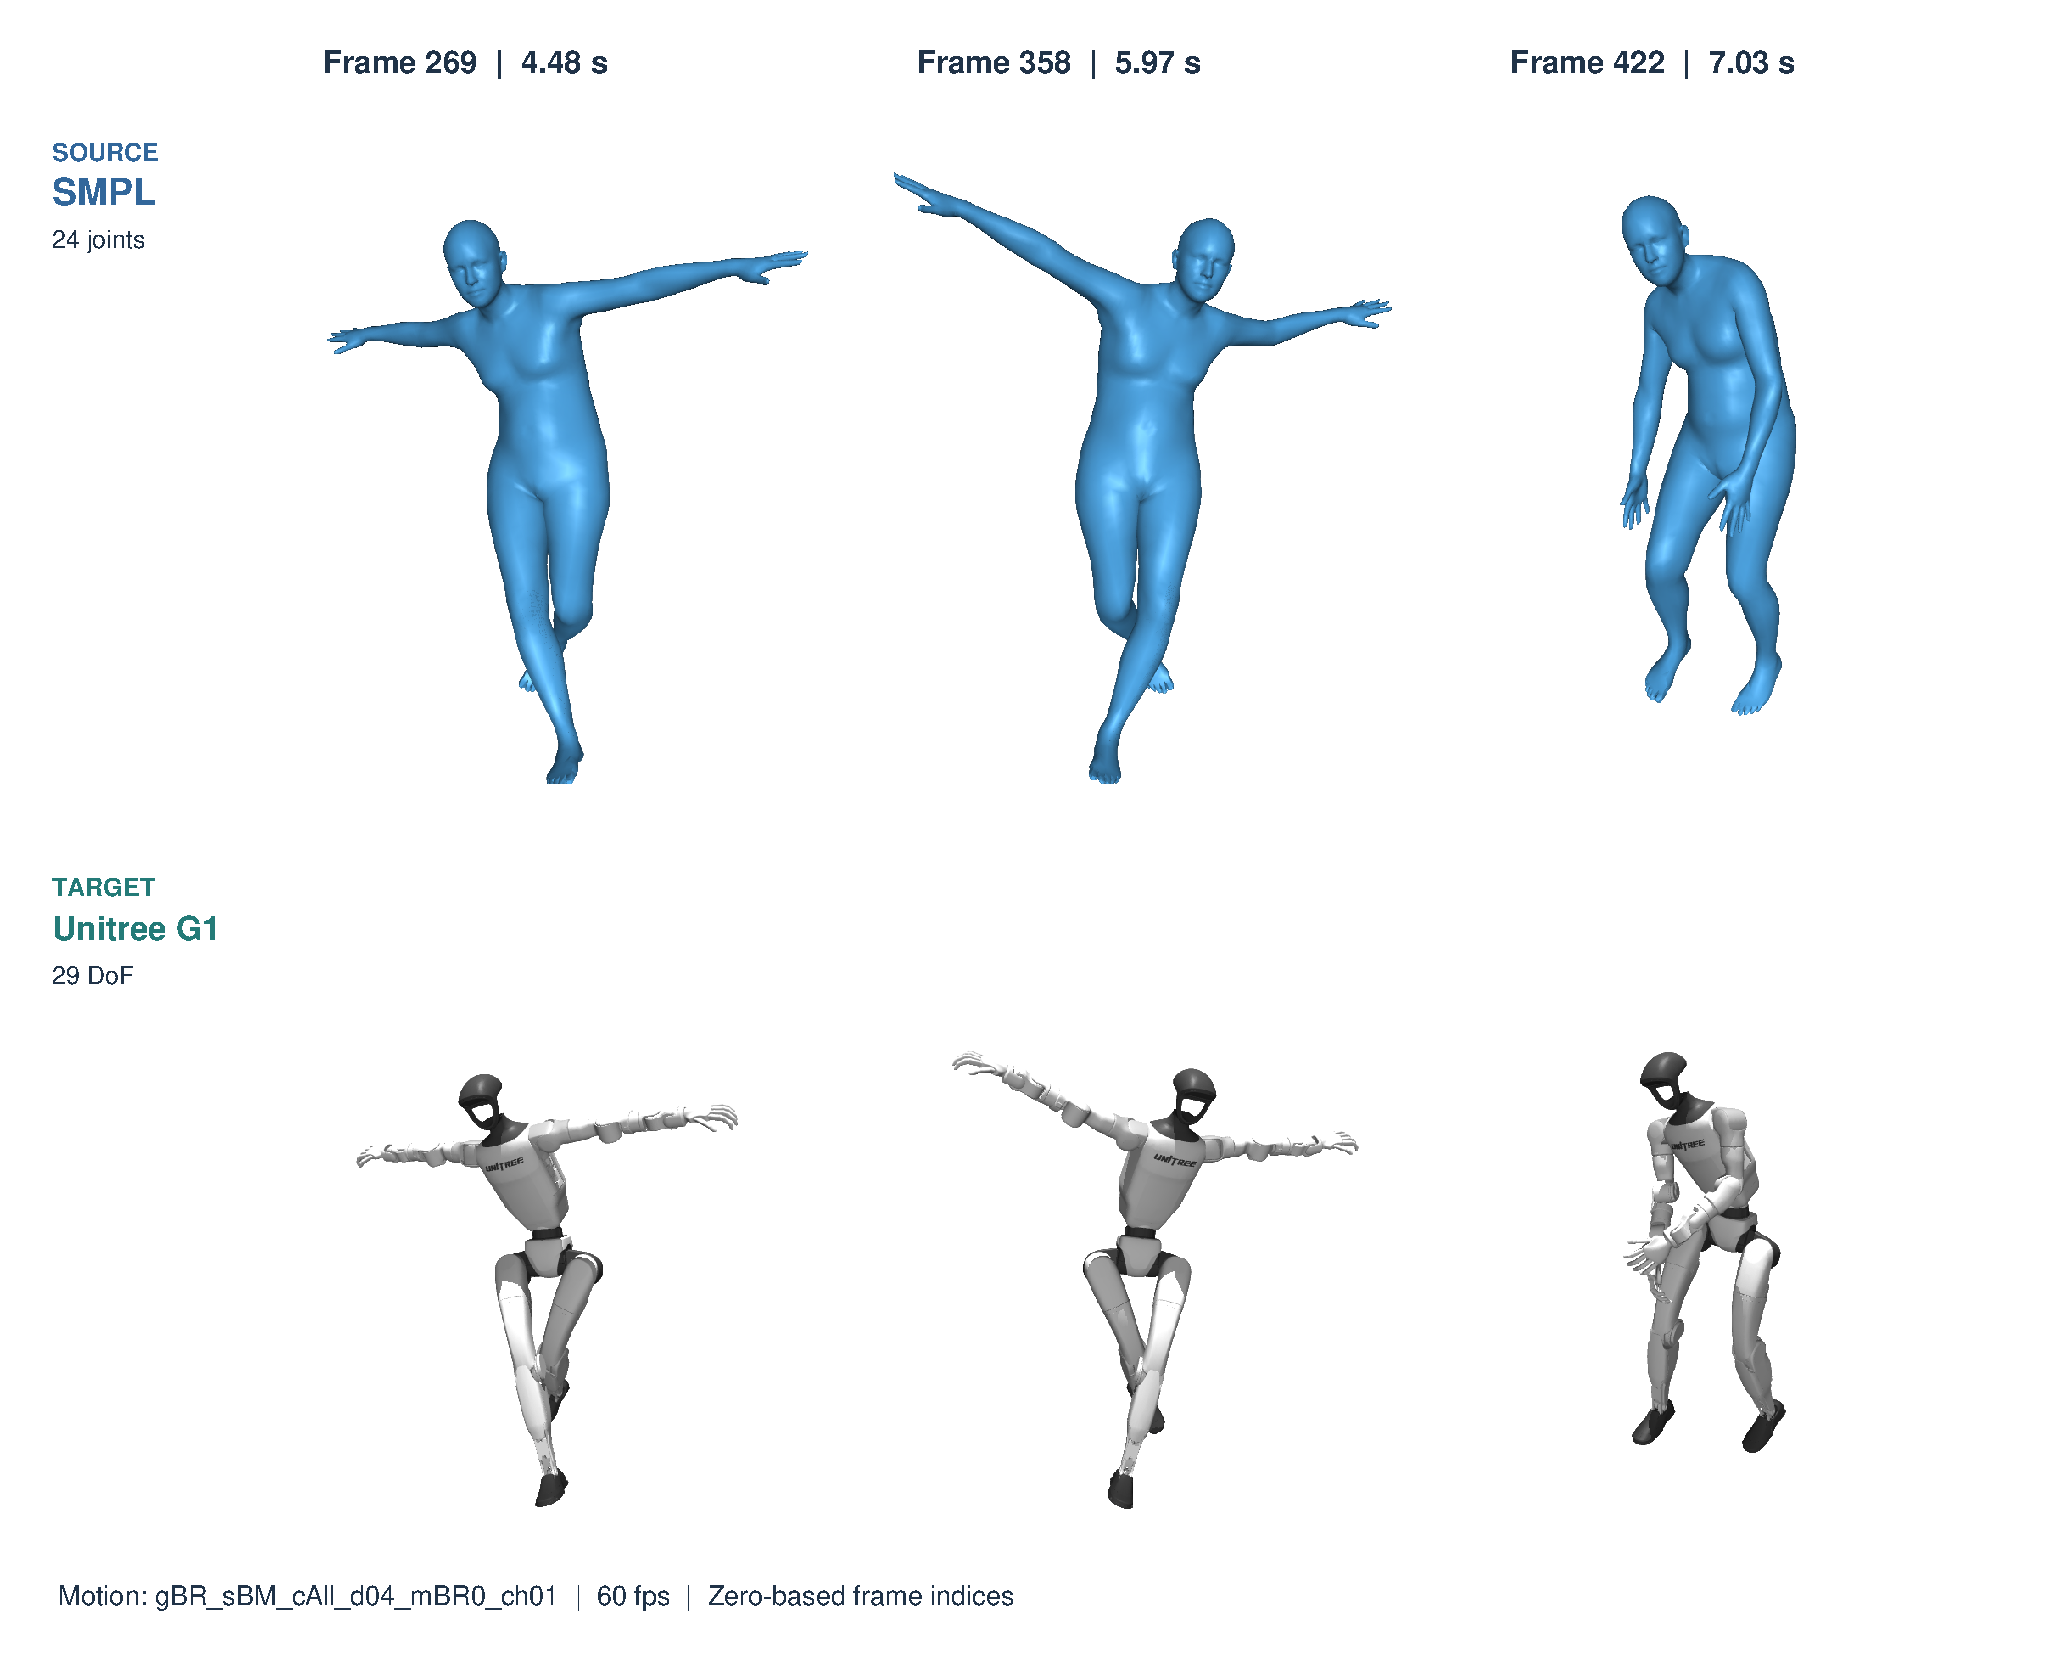
\includegraphics[width=\textwidth]{figures/chapter4_smpl_g1_same_frame.pdf}
    \caption{Same-frame SMPL-to-G1 retargeting comparison for AIST++ sequence
    \texttt{gBR\_sBM\_cAll\_d04\_mBR0\_ch01}. The neutral SMPL source mesh
    (top) and stored GMR-retargeted G1 poses (bottom) are shown at zero-based
    frames 269, 358, and 422 of the 60~fps sequence. Each column uses the same
    frame, camera, and metric scale. For display, each body is independently
    centred horizontally and grounded vertically; joint rotations are
    unchanged, so absolute root translation and ground clearance are not
    compared. Source and SMPL-model hashes were verified against the target
    artefact.}
    \label{fig:smpl_g1_same_frame}
\end{figure}

\subsection{Human forward kinematics and coordinate conversion}
\label{subsec:human_fk}

The AIST++ pose at each frame contains local axis--angle rotations for the 24
SMPL joints and, when available, root translation. Retargeting individual local
angles directly would ignore the different kinematic trees and proportions of
the human and robot. The implementation therefore composes rotations through
the complete SMPL hierarchy to obtain world-space joint positions and
orientations. Root translation is divided by the sequence's SMPL scale before
being applied.

AIST++/SMPL motion is expressed in a $Y$-up convention, whereas the target
MuJoCo model is $Z$-up. Positions and orientations are transformed by

\begin{equation}
    C_{Y\rightarrow Z}=
    \begin{bmatrix}
        1 & 0 & 0\\
        0 & 0 & -1\\
        0 & 1 & 0
    \end{bmatrix}.
    \label{eq:yup_to_zup}
\end{equation}

World rotations are converted to scalar-first quaternions
$[q_w,q_x,q_y,q_z]$. Because $\mathbf{q}$ and $-\mathbf{q}$ encode the same
rotation, quaternion signs are made temporally continuous. This apparently
small step is essential: an untreated sign flip appears as a large angular
change to interpolation and velocity calculations even though the physical
orientation is unchanged.

Fourteen human transforms are supplied as GMR targets: pelvis, upper spine,
left and right hips, knees, feet, shoulders, elbows, and wrists. This subset
captures root placement, leg contacts, torso orientation, and expressive arm
motion while leaving GMR to resolve the different source and target skeletons.
The method follows the general principle that retargeting quality materially
affects the feasibility of subsequent humanoid tracking
\cite{araujo2025retargeting}.

\subsection{GMR inverse-kinematics solve}
\label{subsec:gmr_solve}

The target is the free-root Unitree G1 model with 29 actuated joints. For every
source frame, GMR solves a constrained inverse-kinematics problem that balances
the selected human transforms against the robot kinematic structure and joint
limits. The implementation uses the DAQP-based solver with velocity limiting.
A symmetric two-step arm seed is applied before the sequence solve to reduce
the risk that the nonlinear optimiser enters a mirrored arm configuration.

Reproducibility requires control of library interfaces as well as data files.
The checked GMR revision expects an earlier positional form of the Mink
inverse-kinematics API, whereas the installed Mink version assigns a different
meaning to the corresponding argument. A narrow compatibility adapter maps the
call explicitly and records the detected limits-API mode in every artefact.
Without this adapter, the program can either fail at runtime or, more
dangerously, run with constraints in the wrong parameter position. The adapter
is kept at the integration boundary rather than modifying the optimisation
algorithm.

\subsection{Collision-aware retargeting}
\label{subsec:collision_retargeting}

Pose matching alone can place a robot hand through its torso or allow opposite
limbs to intersect. Collision avoidance is therefore enabled during trajectory
generation. The project's G1 self-collision preset defines nine groups of
non-adjacent body pairs. Adjacent links are omitted because their meshes
naturally overlap around a joint and would create persistent false constraints.
Hand geometries that are visual-only in the source model are activated for
collision evaluation.

The current preset uses a $5\,\mathrm{mm}$ minimum separation, an
$80\,\mathrm{mm}$ detection distance, a gain of $0.85$, and no constraint-bound
relaxation. Validation uses a $6\,\mathrm{mm}$ separation requirement, providing
a $1\,\mathrm{mm}$ numerical buffer beyond the generation constraint. The
expanded preset currently yields 226 geometry pairs, although this count is
recorded rather than assumed because a robot-model revision may change the
geometry set.

Collision validity is checked against both the GMR retargeting model and the
MuJoCo playback model. This dual-model check matters because different XML
files can use different meshes, contact exclusions, or visual/collision roles.
Where shallow contact behaviour differs between MuJoCo versions, the validator
uses explicit geometry-distance queries so that the intended separation
contract remains visible. The scope of this kinematic validation is stated with
the complete preflight procedure in Section~\ref{subsec:mujoco_preflight}.

\subsection{Continuity conditioning}
\label{subsec:retarget_continuity}

Even a collision-free per-frame solution can contain an abrupt change between
neighbouring frames. After retargeting, joint positions are first clamped for
minor numerical overshoot beyond their model limits. Root quaternions are
renormalised and their signs are made continuous. Segment velocities are then
limited to

\begin{equation}
    \|\dot{\mathbf{q}}_{\mathrm{joint}}\|_{\infty}
        \leq 3\pi\;\mathrm{rad\,s^{-1}},\qquad
    \|\dot{\mathbf{p}}_{\mathrm{root}}\|_2
        \leq 3\;\mathrm{m\,s^{-1}},
    \label{eq:retarget_linear_limits}
\end{equation}

and root angular speed is limited to $4\pi\,\mathrm{rad\,s^{-1}}$. For a
violating segment, the correction is not accepted solely from endpoint tests.
The candidate interpolation is sampled at 40 intermediate poses and checked
against the collision constraints. A 14-iteration binary line search finds the
largest safe progress towards the proposed frame. Two stabilisation passes are
used because restricting one segment changes the starting state of the next.
If the first retargeted frame is colliding, it is backed off towards the neutral
configuration.

This stage conditions the source trajectory but does not close its loop. A
forced last-to-first match would change valid one-shot motion and hide the real
seam that the online transition controller must handle. Loop suitability and
clip-to-clip blending are therefore addressed during playback.

\section{Canonical Trajectory and Dataset Build}
\label{sec:canonical_dataset}

\subsection{Canonical G1 artefact}
\label{subsec:canonical_artifact}

Each successfully retargeted dance is stored as a canonical binary artefact.
Its primary arrays are

\begin{equation}
    \mathbf{P}\in\mathbb{R}^{N\times3},\qquad
    \mathbf{Q}_{r}\in\mathbb{R}^{N\times4},\qquad
    \mathbf{Q}_{j}\in\mathbb{R}^{N\times29},
    \label{eq:canonical_motion_arrays}
\end{equation}

representing root position, root orientation in \texttt{wxyz} order, and G1
joint positions. The stored joint-name list fixes the semantic order of all 29
columns. Array width alone is insufficient because two 29-DoF models may use a
different order. The artefact also stores frame rate, format and pipeline
versions, source identifier and digest, SMPL-model digest, retargeter name and
full revision, collision settings, compatibility mode, and continuity limits.


\subsection{Cached builds, quarantine, and atomic publication}
\label{subsec:dataset_build_management}

Retargeting hundreds of clips is expensive, so the builder supports validated
reuse. Before reuse, a cached artefact is checked for the expected schema,
source and model hashes, complete GMR revision, frame rate, joint order,
quaternion convention, collision preset, and continuity settings. Array shapes,
finite values, quaternion norms, and sign continuity are checked as well. A
file that fails validation is renamed with an \texttt{.invalid} suffix rather
than being left under its canonical name.

New trajectories are generated to a temporary \texttt{.build} path. Only a
fully validated output atomically replaces the canonical path. Dataset
manifests follow the same publish-after-validation rule. A complete build of an
official split may replace its manifest. A partial build is merged so that an
interrupted experiment does not erase unrelated valid rows. Failed identifiers
are removed from the active manifest and written to a separate failure report.

These measures turn the manifest into a declaration of validated availability.
They also make interrupted builds recoverable. The
next run can reuse verified artefacts, quarantine incompatible ones, and
continue without assuming that an existing filename is complete.

\section{Trajectory Preflight and Catalogue Admission}
\label{sec:preflight_admission}

\subsection{MuJoCo kinematic preflight}
\label{subsec:mujoco_preflight}

The catalogue builder treats trajectory loading as a testable operation. The
preflight validator first repeats the canonical schema and provenance checks.
It rejects non-finite arrays, an unexpected joint order, invalid quaternion
norms, missing source identity, disabled collision generation, or an abbreviated
software revision. It also applies secondary corruption thresholds of
$20\,\mathrm{rad\,s^{-1}}$ for joint speed, $10\,\mathrm{m\,s^{-1}}$ for root
translation, and $20\,\mathrm{rad\,s^{-1}}$ for root angular speed. These are
looser than the generation limits in Section~\ref{subsec:retarget_continuity}.
Their role is to detect malformed data.

The trajectory is then loaded into the headless G1 playback model and grounded.
For each frame, the validator checks finite joint values and actual model joint
ranges. At a fixed stride of four frames it writes the kinematic state into
MuJoCo and calls forward evaluation. Generalised position, velocity, and
actuator-state arrays must remain finite, and the minimum foot height must not
fall below $-10^{-5}\,\mathrm{m}$ after grounding. No actuator command is
applied in this test.

Preflight is therefore a kinematic admission test. It catches schema mismatch, model-order
errors, invalid states, excessive discontinuities, and grounding failure at
catalogue-build time. Dynamic tracking, torque limits, balance, and hardware
safety require a later controller and a separate experimental evaluation.

\subsection{Joining audio and motion records}
\label{subsec:catalogue_join}

After preflight, the builder joins each valid motion profile to its music
segments. A row enters the searchable catalogue only if the audio source,
source SMPL motion, canonical G1 artefact, key-pose profile, and preflight result
are all present. Excluded rows are written to a dedicated CSV file with a
machine-readable reason. This strict inner join prevents a high-scoring audio
entry from referring to a motion that the online process cannot load.

The current catalogue contains 411 paired manifest
rows. All 411 motion rows passed admission in the recorded build, with zero
excluded motions. Because several dances share music, these rows refer to 60
music identifiers, 70 representative audio variants, and 348 audio segments.
The global median equivalent motion speed is approximately
$1.31\,\mathrm{m\,s^{-1}}$. These figures document the current artefact. A rebuild with different data, model
weights, or validation settings must update them.

\section{Integrity Guarantees and Remaining Limitations}
\label{sec:offline_integrity}

The finished offline catalogue provides five guarantees to the online matcher.
First, the query and reference audio paths share one documented extractor and
one learned-model identity, so their descriptors are compared within a
consistent feature space. Second, dense matrices have known dimensions and
reference-set normalisation statistics, preserving comparability across live
queries. Third, every selectable motion has stable source and retargeting
provenance, including source and model hashes, software revision, and generation
settings. Fourth, key poses and activity statistics have been computed
consistently from the source sequence, providing comparable entry candidates
and motion profiles. Fifth, the exact trajectory can be loaded, grounded, and
evaluated in the target MuJoCo kinematic model, with its joint ordering,
numerical validity, and model compatibility checked before admission.

Together, these guarantees establish a traceable connection between an audio
retrieval result and an available robot trajectory. Validated caching,
quarantine of incompatible artefacts, and atomic publication reduce the risk
of exposing stale or incomplete outputs. The final audio--motion join further
ensures that searchable entries refer to motions with the required profiles
and preflight results. These guarantees remain specific to the recorded data,
model assets, and validation settings. Changes to those dependencies require
the corresponding artefacts to be rebuilt or revalidated.

But these guarantees stop short of several stronger claims. A
Discogs-derived embedding is not a direct measure of choreographic correctness:
musical similarity does not establish that a particular motion suits the
phrasing or expressive intent of a new passage. A velocity valley is not
necessarily a semantic dance boundary, and a low-velocity source pose does not
by itself guarantee a smooth transition from the robot's current state.
Retargeting and continuity conditioning may also alter the motion around a
source-derived key pose, so entry suitability still requires online evaluation.

IK and self-collision constraints do not prove balance, torque feasibility, or
safe hardware execution. The MuJoCo preflight evaluates kinematic states
without applying actuator commands, and its sampled checks do not establish
continuous-time dynamic feasibility. Likewise, validating individual clips
does not validate every possible blend, loop seam, or playback-speed change.
Finally, AIST++ pairings reflect the choreography in the dataset and may not
cover arbitrary live music or all desired G1 behaviours.



% Chapter 5 can be included from a larger thesis with \input or \include.
% Citation keys are maintained in references.bib.

\chapter{Real-Time Music--Motion Matching and Continuous Control}
\label{chap:realtime_matching_control}

\section{Chapter Overview}
\label{sec:ch5_overview}

Chapter~\ref{chap:offline_catalogue} constructed a catalogue in which every
audio reference has a consistent descriptor and every selectable dance has a
preflight-passed Unitree G1 trajectory. This chapter develops the online method
that uses this catalogue. The method receives an audio stream, retrieves
musically related references, ranks their associated motions, accumulates
evidence for a stable selection, and connects the selected trajectory to the
currently playing one. At the same time, a causal beat controller adjusts
motion phase without discontinuously jumping between poses.

The proposed method is retrieval-based rather than generative. It cannot create
an unseen choreography, but it offers three practical advantages for the
present humanoid system. First, the source of every commanded pose is known.
Second, expensive retargeting and preflight are completed before live use.
Third, retrieval, selection, timing, and transition errors can be measured
separately. These properties complement recent work on expressive audio-driven
humanoid locomotion and streaming character generation, which demonstrates the
importance of musical responsiveness but also highlights the difficulty of
causal control \cite{li2026you,ji2026discoforcing}.

The online method is organised around three different decisions:

\begin{enumerate}[label=(\arabic*)]
    \item \emph{what} music and motion are supported by the recent audio.
    \item \emph{when} the evidence is stable enough to authorise a switch.
    \item \emph{how} the current and selected robot trajectories can be joined
          without a pose, velocity, contact, or root discontinuity.
\end{enumerate}



\section{Online Problem Formulation}
\label{sec:ch5_problem}

Let $\mathcal{A}_{\leq t}$ denote audio observed up to current time $t$, and let
$\mathcal{M}=\{M_i\}_{i=1}^{N}$ be the finite catalogue of robot-ready
motions. Each $M_i$ is associated with source music $u_i$, an authored tempo,
an activity profile, key-pose phases, foot-contact states, and a G1 trajectory.
The online system selects motion $M_{i_t}$ and phase $\phi_t$, then produces
the emitted configuration $\mathbf{q}^{\mathrm{out}}_t$ using only
$\mathcal{A}_{\leq t}$ and stored state:

\begin{equation}
    \bigl(i_t,\phi_t,\mathbf{q}^{\mathrm{out}}_t\bigr)
    =\mathcal{G}\!\left(\mathcal{A}_{\leq t},\mathcal{M},\mathcal{H}_{t}\right),
    \label{eq:ch5_causal_mapping}
\end{equation}

where $\mathcal{H}_{t}$ contains the current motion, recent rankings, accepted
beats, played-motion history, prepared candidates, and controller state. The
history term makes explicit that selection is stateful. Applying a memoryless
nearest-neighbour rule independently to every window would make
$i_t$ oscillate when several catalogue items have similar scores.

Throughout the thesis, $\mathcal{F}$ denotes audio feature extraction and
$\mathcal{G}$ denotes stateful online control. The waveform history
$\mathcal{A}_{\leq t}$ is distinct from its descriptor $\mathbf{x}_t$.
The full catalogue $\mathcal{D}$ contains descriptors, trajectories $M_i$ and
metadata $\mathbf{m}_i$; $\mathcal{M}$ is its trajectory collection, and
$\mathcal{C}_t$ is the ranked motion candidate set. Thus $\mathbf{x}_i$ and
$M_i$ denote different parts of an item, rather than alternative names for it.
The index $i_t$ identifies the selected motion, $\phi_t$ is playback phase,
and $\mathbf{q}^{\mathrm{out}}_t$ is the emitted robot configuration after
blending and output constraints. The time subscript refers to the current
update instant; $\Delta t$ is the elapsed time between updates.

The method optimises no single end-to-end objective at runtime. Instead, it
uses a sequence of constrained local objectives:

\begin{equation}
\begin{aligned}
    &\text{audio retrieval:} &&\max s_{\mathrm{track}},\\
    &\text{motion ranking:}  &&\max s_{\mathrm{final}},\\
    &\text{entry search:}    &&\min C_{\mathrm{entry}},\\
    &\text{playback:}        &&\min |e_{\phi}|\quad
       \text{subject to phase-rate and output constraints}.
\end{aligned}
    \label{eq:ch5_local_objectives}
\end{equation}

This factorisation reflects the available evidence. Audio descriptors can
indicate semantic and rhythmic compatibility, but they cannot determine the
instantaneous joint configuration at which a switch is smooth. Conversely,
joint-space entry cost cannot decide whether a dance is appropriate for the
music.

\subsection{Dual-timescale causal processing}
\label{subsec:ch5_dual_timescale}

The same audio stream is processed at two timescales. A six-second rolling
waveform supplies the context required by the catalogue extractor. A retrieval
attempt is made once per second when the previous attempt has completed. In
parallel, a short-block analyser emits activity, onset, spectral, and beat
events used for phase control and subtle pose modulation. The retrieval view
therefore estimates musical identity and compatibility, whereas the event view
estimates local timing.

Both paths are causal. No sample later than the current audio position is used.
This is stricter than merely playing an offline model incrementally, a
distinction emphasised in real-time diffusion control
\cite{ji2026discoforcing}. The longer retrieval window does introduce an
observation delay at startup and after a musical change. This delay is explicit
and can be measured. It is not hidden by using future context.

Feature extraction and catalogue search run in a single background worker. If
that worker is occupied, the next submission opportunity is skipped. Requests
are not accumulated in a queue. Thus the live controller consumes the newest
completed evidence instead of processing an increasing backlog of stale audio
windows. Completed rankings are passed to the bounded candidate-preparation
subsystem described in Section~\ref{subsec:ch5_commitment_readiness}.

\section{Hierarchical Music-to-Motion Retrieval}
\label{sec:ch5_hierarchical_retrieval}

\subsection{Query standardisation and segment similarity}
\label{subsec:ch5_segment_similarity}

For every query window, the online extractor produces the same three vectors
as the offline pipeline: a learned embedding $\mathbf{e}_q$, a rhythm--timbre
vector $\mathbf{r}_q$, and style activations $\mathbf{g}_q$. The embedding is
derived from the same Discogs EffNet model used to construct the catalogue
\cite{alonso2022music}. Model identity and feature dimensions are checked at
startup. A mismatch is treated as an error.

Learned and rhythm vectors are standardised using the catalogue statistics and
then normalised to unit length. For feature family $f\in\{e,r\}$,

\begin{equation}
    \overline{\mathbf{f}}_q=
    \frac{(\mathbf{f}_q-\boldsymbol{\mu}_f)
          /\max(\boldsymbol{\sigma}_f,\epsilon)}
         {\left\|(\mathbf{f}_q-\boldsymbol{\mu}_f)
          /\max(\boldsymbol{\sigma}_f,\epsilon)\right\|_2}.
    \label{eq:ch5_query_standardisation}
\end{equation}

Style activations are unit-normalised without z-standardisation because their
coordinates have a direct label meaning. Cosine similarity is mapped into
$[0,1]$:

\begin{equation}
    s_f(q,n)=\frac{1+\overline{\mathbf{f}}_q^{\mathsf{T}}
        \overline{\mathbf{f}}_n}{2}.
    \label{eq:ch5_mapped_cosine}
\end{equation}

For catalogue segment $n$, the fused score is

\begin{equation}
    s_{\mathrm{seg}}(q,n)
    =0.70s_e(q,n)+0.20s_r(q,n)+0.10s_g(q,n).
    \label{eq:ch5_segment_fusion}
\end{equation}

The learned representation supplies the main semantic neighbourhood, while
explicit rhythm prevents two stylistically similar but rhythmically dissimilar
passages from being treated as identical. Style activations have the smallest
weight because they are useful priors but are too coarse to determine a track
on their own. If style-vector dimensions are unavailable, the remaining
weights are renormalised to $0.70/0.90$ and $0.20/0.90$. Missing evidence is
not interpreted as zero similarity.

\subsection{Track pooling and genre-first restriction}
\label{subsec:ch5_track_pooling}

A track normally contributes several overlapping catalogue segments. Using its
single best segment is sensitive to accidental local agreement, whereas an
average over the entire track penalises longer recordings and music with
legitimate internal variation. Let
$s_{u,(1)}\geq s_{u,(2)}\geq\cdots$ be the ordered segment scores belonging to
track $u$. The track score is the mean of at most the three highest values:

\begin{equation}
    s_{\mathrm{track}}(q,u)
    =\frac{1}{K_u}\sum_{k=1}^{K_u}s_{u,(k)},
    \qquad K_u=\min(3,N_u).
    \label{eq:ch5_track_pooling}
\end{equation}

Tracks are next grouped by their AIST++ genre code. An initial genre score is
the same top-three mean over tracks in that genre. Discogs labels are also
mapped to broad AIST++ families. For example, hip-hop labels support the
middle- and low-hip-hop families, while house and techno labels support the
house family. These mappings are deliberately broad priors rather than a claim
that Discogs and AIST++ define identical taxonomies.

When the largest mapped tag prior is at least $0.08$, the final genre score is

\begin{equation}
    s_{\mathrm{genre}}(h)
    =0.35\,\widetilde{s}_{\mathrm{track\mbox{-}genre}}(h)
     +0.65\,\widetilde{p}_{\mathrm{tag}}(h),
    \label{eq:ch5_genre_prior}
\end{equation}

where both terms are normalised within the current query. The default
style-first policy admits the highest-scoring family. It also admits the second
family when the genre-score margin is no more than $0.025$. All later motion
ranking is restricted to admitted families and to tracks among the retrieved
set. This hierarchy reduces an important failure mode of flat retrieval. A
small acoustic advantage from an unrelated genre cannot be compensated later
by a mechanically convenient motion.

\subsection{Abstention and match confidence}
\label{subsec:ch5_abstention}

The system is allowed to abstain. It computes a negative-style score as the
largest activation among non-music, ambient, drone, field-recording, noise, and
related tags. If this value is at least $0.17$ for two consecutive retrieval
windows, the query is rejected as non-dance or ambient material. Persistence
prevents one uncertain tag activation from cancelling a valid dance selection.
A query is also rejected when the beat-quality value defined in
Equation~\ref{eq:beat_quality} is below $0.35$.

For diagnostics, confidence combines beat quality $q_b$ and the leading genre
margin $\Delta_h$:

\begin{equation}
    c_{\mathrm{match}}
    =\operatorname{clip}_{[0,1]}\!\left(
       0.55q_b+0.45\operatorname{clip}_{[0,1]}
       \left(\frac{\Delta_h}{0.10}\right)
      \right).
    \label{eq:ch5_match_confidence}
\end{equation}

This confidence value explains the strength of the evidence but does not
override the explicit rejection rules. When a result is rejected, no new
motion evidence is accumulated and the current motion remains active. Therefore, the
system fails by holding a known trajectory.

\subsection{Motion-specific compatibility}
\label{subsec:ch5_motion_compatibility}

Music retrieval identifies relevant recordings, but each recording can be
associated with several dances that differ in speed, event density, and
activity. A second ranking stage evaluates the motion itself. Only motions
whose offline preflight passed and whose music and genre survived the preceding
stage are considered.

Tempo compatibility handles half-time and double-time ambiguity. For query BPM
$b_q$ and the source tempo $b_i$ of motion $M_i$, the candidate playback ratios
are

\begin{equation}
    \mathcal{R}_i=
    \left\{\frac{b_q}{b_i},\frac{b_q}{2b_i},
                  \frac{2b_q}{b_i}\right\}.
    \label{eq:ch5_tempo_ratios}
\end{equation}

Only ratios in $[0.55,1.60]$ are retained. The valid ratio closest to one in
log space is selected, and its compatibility is

\begin{equation}
    s_{\mathrm{tempo}}(i)
    =\exp\!\left[-\frac{1}{2}
      \left(\frac{\log r_i}{0.28}\right)^2\right].
    \label{eq:ch5_tempo_score}
\end{equation}

If no ratio is feasible, the motion is excluded. If reliable tempo is absent,
the implementation assigns a deliberately weak score of $0.25$ at authored
speed.

Rhythmic compatibility compares the audio event rate with the motion key-pose
rate. The query and motion rates are

\begin{equation}
    \rho_q=0.70\frac{b_q}{60}+0.30d_o,
    \qquad
    \rho_i=r_i d_{k,i},
    \label{eq:ch5_event_rates}
\end{equation}

where $d_o$ is onset density and $d_{k,i}$ is confidence-weighted key-pose
density. Their scale-symmetric agreement and the motion regularity term are

\begin{align}
    s_{\mathrm{density}}(i)
      &=\exp\!\left[-\frac{1}{2}
        \left(\frac{|\log(\rho_i/\rho_q)|}{0.65}\right)^2\right],\\
    s_{\mathrm{key}}(i)
      &=0.80s_{\mathrm{density}}(i)
        +0.20\exp\!\left[-\min(c_{v,i},2)\right].
    \label{eq:ch5_keypoint_score}
\end{align}

When either rate is effectively zero, $s_{\mathrm{key}}=0.25$. This avoids an
undefined logarithm while preserving the uncertainty penalty.

Motion activity is obtained from the catalogue-relative 90th-percentile
velocity. With catalogue median $\mu_v$ and robust scale $\sigma_v$,

\begin{equation}
    a_i=\frac{1}{1+\exp[-(v_{90,i}-\mu_v)/\sigma_v]},
    \qquad
    s_{\mathrm{activity}}(i)=1-|a_q-a_i|,
    \label{eq:ch5_activity_score}
\end{equation}

where $a_q$ is the audio activity from
Equation~\ref{eq:audio_activity}. The complete motion and final scores are

\begin{align}
    s_{\mathrm{motion}}(i)
      &=0.50s_{\mathrm{tempo}}(i)
        +0.35s_{\mathrm{key}}(i)
        +0.15s_{\mathrm{activity}}(i),\\
    s_{\mathrm{final}}(i)
      &=0.65s_{\mathrm{track}}(u_i)
        +0.35s_{\mathrm{motion}}(i).
    \label{eq:ch5_final_motion_score}
\end{align}

Music evidence remains dominant, but the motion-specific term prevents a
semantically similar track from authorising choreography that would require
extreme time scaling or has incompatible event density. All component values
are retained for evaluation and ablation.

\section{Stable Selection and Candidate Readiness}
\label{sec:ch5_stable_selection}

\subsection{Relevance hysteresis}
\label{subsec:ch5_relevance_hysteresis}

Let $i_t^{*}$ be the leading motion at retrieval update $t$, and let $i_c$ be
the currently playing motion. A relevance switch is armed only when

\begin{equation}
    i_t^{*}\neq i_c,
    \qquad
    s_{\mathrm{final}}(i_t^{*})
       \geq s_{\mathrm{final}}(i_c)+0.08,
    \label{eq:ch5_relevance_margin}
\end{equation}

for three consecutive completed retrievals with the same $i_t^{*}$. If the
leader changes, the current motion becomes best, the score margin disappears,
or the match is rejected, the streak is reset. A successful streak creates a
\emph{pending relevance selection}. It does not immediately alter playback.

This hysteresis is important because overlapping audio windows are strongly
correlated. Three wins should not be interpreted as three independent
statistical observations. They are instead a temporal persistence rule that
filters short score inversions while giving sustained evidence a bounded path
to a switch.

\subsection{Diversity under a relevance constraint}
\label{subsec:ch5_diversity_selection}

A stable musical passage can keep the same motion at rank one for a long time.
To avoid visible repetition, diversity is handled by a second policy. It
considers the latest top five motions and retains only candidates satisfying

\begin{equation}
\begin{aligned}
    s_{\mathrm{final}}(i)&\geq s_{\mathrm{final}}(i^{*})-0.05,\\
    s_{\mathrm{track}}(u_i)&\geq s_{\mathrm{track}}(u_{i^{*}})-0.08.
\end{aligned}
    \label{eq:ch5_diversity_eligibility}
\end{equation}

The candidate must remain eligible for the same three-update streak. After the
current motion has been held for four accepted-beat bars, the selector first
prefers a motion cluster absent from the three-item recent history, then an
unseen motion identifier, and finally the least recently played eligible item.
The score constraints are applied before recency, so variation cannot introduce
an arbitrarily poor match.

Relevance and diversity selections record different reasons. A relevance
selection can be committed at the next valid boundary as soon as it is ready.
A diversity selection is committed only after the maximum hold has actually
been reached. This distinction allows a genuine musical change to take
priority over a cosmetic rotation.

\subsection{Accepted-beat commitment and prepared candidates}
\label{subsec:ch5_commitment_readiness}

The switch clock counts accepted alignment beats rather than raw detector
peaks. Every four accepted beats defines a bar boundary. A pending selection
becomes eligible for commitment at this boundary, ensuring that switching and
phase control share one rhythmic interpretation. The logical state progression
is

\begin{equation}
    \texttt{current}\rightarrow\texttt{evidence}
    \rightarrow\texttt{pending}\rightarrow\texttt{prepared}
    \rightarrow\texttt{transitioning}\rightarrow\texttt{current}.
    \label{eq:ch5_selection_states}
\end{equation}

Whenever a ranking arrives, the pending motion and other high-ranked motions
are submitted to a bounded preparation pool. Preparation includes canonical
trajectory loading, grounding in the playback model, joint-name adaptation,
and construction of the entry features used in
Section~\ref{sec:ch5_entry_optimisation}. As a bar boundary approaches, ready
candidates are scored against an estimate of the source phase expected at that
boundary.

The pending identifier remains the preferred choice whenever it is fully
prepared. Entry cost chooses the best phase within that motion. It does not
silently replace a musically preferred motion with a less relevant one. If the
preferred motion is not ready, a different ranked and prepared candidate may be
used as an explicit fallback. If no evidence-backed candidate is ready, the
system continues the current trajectory. File I/O and grounding are never
performed synchronously merely to meet a boundary.

\section{Causal Beat and Phase Control}
\label{sec:ch5_beat_phase_control}

\subsection{Activity gate and beat candidates}
\label{subsec:ch5_beat_candidates}

Microphone startup includes a short calibration from which the 90th percentile
of RMS and onset change estimates the local noise floor. Subsequent audio is
active only when its RMS exceeds both a fixed floor and a multiple of the
calibrated floor. A short release interval prevents the activity state from
chattering near the threshold. When audio is inactive, beat history is reset
and motion amplitude returns gradually towards zero.

Beat candidates are produced by predominant local pulse (PLP) estimation,
following Grosche and M\"uller \cite{grosche2010extracting}.
The implementation uses the librosa library \cite{mcfee2015librosa}, applying
\texttt{librosa.beat.plp} to a rolling history of already acquired audio.
PLP combines locally estimated periodicities
into a pulse curve; its peaks supply beat candidates. Block-level onset and
loudness histories supply local event contrast. Analysis can revise estimates
inside its available window, but the controller acts only when results are
delivered and cannot revise emitted poses. This online PLP path is distinct
from the dynamic-programming beat tracker used for catalogue descriptors
\cite{ellis2007beat}. In the present method,
each candidate has pulse confidence $c_p$ and recent-event contrast $c_x$. Its
selection score is

\begin{equation}
    c_b=(1-w_x)c_p+w_xc_x,
    \qquad w_x=0.5.
    \label{eq:ch5_beat_selection_score}
\end{equation}

Candidates below the hard confidence threshold $c_p<0.35$ are rejected before
they can influence phase or the bar counter.

\subsection{Motion-aware beat acceptance}
\label{subsec:ch5_beat_acceptance}

Dense music may contain subdivisions faster than the current dance can travel
between authored key poses. The controller therefore derives an admissible
time interval from the next key-pose gap $T_k$ and the playback-speed limits:

\begin{equation}
    T_{\min}=\eta\frac{T_k}{r_{\max}},
    \qquad
    T_{\max}=\frac{T_k}{r_{\min}},
    \label{eq:ch5_beat_time_window}
\end{equation}

where $\eta$ is the key-point interval ratio and is one in the current matcher
configuration. A beat earlier than $T_{\min}$ after the previous accepted beat
is rejected. When the detector itself proposes periods shorter than this
feasible interval, recent candidate scores define an adaptive quantile
threshold. Weak subdivisions are rejected early in the admissible window. The
threshold falls as elapsed time approaches $T_{\max}$. At the deadline, an
eligible beat is accepted so that the controller cannot wait indefinitely for
an ideal accent.

This policy treats beat detection and beat use as different problems. The
analyser may report all plausible pulses, but only events compatible with the
motion's next authored interval become control targets. Beat-synchronised dance
methods likewise demonstrate that temporal correspondence must be represented
explicitly rather than inferred from visual plausibility alone
\cite{huang2024beat}.

\subsection{Target rate and gradual phase correction}
\label{subsec:ch5_phase_correction}

For accepted beat index $k$, the controller selects the corresponding authored
key-pose phase $\phi_k^{*}$. The wrapped phase error is

\begin{equation}
    e_{\phi}=\operatorname{wrap}_{[-1/2,1/2)}
             \left(\phi_k^{*}-\phi\right).
    \label{eq:ch5_phase_error}
\end{equation}

The first accepted beat uses the full error as a correction request. Later
events use gain $0.25+0.35c_b$, so a high-quality beat creates a stronger but
still gradual correction. In adaptive mode, if $\Delta\phi_k$ is the authored
phase gap and $\Delta t_k$ is the last accepted-beat interval, the target phase
rate is

\begin{equation}
    \omega^{*}=
    \operatorname{clip}_{[r_{\min}\omega_a,r_{\max}\omega_a]}
    \left(\frac{\Delta\phi_k}{\Delta t_k}\right),
    \label{eq:ch5_target_phase_rate}
\end{equation}

where $\omega_a$ is the authored phase rate. The running base rate is
exponentially smoothed towards $\omega^{*}$. Phase correction is not applied by
assigning $\phi\leftarrow\phi_k^{*}$. Instead, the remaining correction $e_r$
is consumed with time constant $\tau_p$:

\begin{equation}
    \Delta\phi_c=e_r\left(1-e^{-\Delta t/\tau_p}\right).
    \label{eq:ch5_desired_phase_correction}
\end{equation}

The correction is clipped so that the effective phase rate remains within the
same speed interval. Its change is also slew-limited. With the resulting
$\omega_{\mathrm{eff}}$, phase evolves continuously as

\begin{equation}
    \phi_{t+1}=\operatorname{wrap}_{[0,1)}
       \left(\phi_t+\omega_{\mathrm{eff}}\Delta t\right).
    \label{eq:ch5_phase_update}
\end{equation}

This mechanism synchronises by temporarily accelerating or decelerating the
authored motion, not by teleporting to a different frame. When beat evidence
times out, the target rate returns to $\omega_a$. When a new motion controller
is created, it inherits the previous tempo, amplitude, beat history, and
effective-rate state, while its phase is initialised at the selected entry.
Thus switching does not restart rhythmic estimation.

\subsection{Bounded pose modulation}
\label{subsec:ch5_pose_modulation}

Timing adaptation preserves the selected trajectory as the primary source of
movement. A secondary modulation layer adds small, zero-centred offsets from
low-, mid-, and high-frequency energy, rhythm density, off-beat ratio, and beat
accent. In the default subtle mode, the authored pose is not multiplied by a
global amplitude. Instead, bounded offsets are applied mainly to the waist,
shoulders, wrists, and knees. For example, high-frequency activity produces a
small alternating wrist and shoulder detail, while low-frequency energy
produces a small knee component.

This layer is intentionally secondary. It improves immediate responsiveness
between slower retrieval updates without changing motion identity or root
trajectory. Because it can create poses not present in the offline artefact,
its result still passes through the output conditioning described in
Section~\ref{sec:ch5_output_conditioning}.

\section{Transition-Entry Optimisation}
\label{sec:ch5_entry_optimisation}

\subsection{Entry candidates and state features}
\label{subsec:ch5_entry_candidates}

Motion matching and motion-graph methods establish the value of comparing
state features at possible transition points
\cite{kovar2023motion,holden2020learned}. The present method uses this principle
only after music has supplied a small candidate set. For each target key pose,
the search includes its central frame and up to three frames on either side.
The neighbouring candidates receive linearly decreasing salience. This local
expansion can find a materially closer robot configuration without turning the
entry search into an unconstrained scan over the whole clip.

At each candidate, the cached state contains named joint positions and
velocities, joint ranges, grounded root position, root tilt after removing yaw,
root linear velocity, root angular speed, and binary left/right foot contacts.
Only joint names shared by source, target, and the output-limits table are used.
The current source phase is mapped to its nearest source frame.

\subsection{Normalised entry cost}
\label{subsec:ch5_entry_cost}

For source frame $s$ and target candidate $j$, joint-pose and velocity costs are

\begin{align}
    C_q(j)&=\sqrt{\frac{1}{D}\sum_{d=1}^{D}
      \left(\frac{q_{j,d}-q_{s,d}}{R_d}\right)^2},\\
    C_v(j)&=\sqrt{\frac{1}{D}\sum_{d=1}^{D}
      \left(\frac{\dot q_{j,d}-\dot q_{s,d}}
      {v_d^{\max}}\right)^2},
    \label{eq:ch5_pose_velocity_costs}
\end{align}

where $R_d$ is the model joint range and $v_d^{\max}$ is the configured speed
limit. Contact cost is the fraction of the two feet whose support states differ:

\begin{equation}
    C_c(j)=\frac{1}{2}\sum_{f\in\{L,R\}}
       \mathbf{1}\!\left[c_{j,f}\neq c_{s,f}\right].
    \label{eq:ch5_contact_cost}
\end{equation}

Root cost averages four separately normalised disagreements:

\begin{equation}
\begin{split}
    C_r(j)=\frac{1}{4}\bigg(&
       \frac{|z_j-z_s|}{0.15}
       +\frac{|\theta_j-\theta_s|}{0.35}
       +\frac{\|\dot{\mathbf{p}}_j-
                    \dot{\mathbf{p}}_s\|_2}{3.0}\\
       &+\frac{|\omega_{r,j}-\omega_{r,s}|}{4\pi}\bigg),
\end{split}
    \label{eq:ch5_root_cost}
\end{equation}

where $\theta$ is non-yaw root tilt. The key-pose term
$C_m(j)=1-s_j$ favours a salient velocity valley. The total entry cost is

\begin{equation}
    C_{\mathrm{entry}}(j)
      =0.45C_q(j)+0.20C_v(j)+0.20C_c(j)
       +0.10C_r(j)+0.05C_m(j).
    \label{eq:ch5_entry_total}
\end{equation}

Pose mismatch receives the largest weight because it is the most immediately
visible discontinuity. Velocity and contact distinguish frames that have a
similar pose but incompatible movement or support. Root state and musical
salience refine the decision without overriding a severe whole-body mismatch.

\subsection{Feasibility and transition duration}
\label{subsec:ch5_entry_feasibility}

An entry with low instantaneous cost can still be unsuitable if it occurs near
the end of a one-shot target. The conservative remaining playback time is

\begin{equation}
    T_{\mathrm{remain}}(j)
      =\frac{(1-\phi_j)T_i}{r_{\max}}.
    \label{eq:ch5_remaining_time}
\end{equation}

It must cover both the transition and at least one remaining bar under the
default configuration. The unquantised transition lower bound is derived from
joint displacement and the same dynamics limits used by the output layer:

\begin{equation}
    T_{\mathrm{raw}}(j)=\max_d\left(
       \frac{1.5|q_{j,d}-q_{s,d}|}{v_d^{\max}},
       \sqrt{\frac{6|q_{j,d}-q_{s,d}|}{a_d^{\max}}}
    \right).
    \label{eq:ch5_transition_lower_bound}
\end{equation}

After enforcing a minimum, the duration is rounded upward to a half-beat
multiple:

\begin{equation}
    T_{\mathrm{tr}}(j)=
    \operatorname{clip}_{[0.35,1.20]}
    \left(
      \left\lceil\frac{\max(0.35,T_{\mathrm{raw}}(j))}{T_b/2}\right\rceil
      \frac{T_b}{2}
    \right).
    \label{eq:ch5_transition_quantisation}
\end{equation}

The candidate is eligible when
$T_{\mathrm{remain}}\geq T_{\mathrm{tr}}+T_{\mathrm{bar}}$. Candidates whose
raw requirement exceeds the maximum transition duration are avoided whenever
a feasible alternative exists. Eligible candidates are ordered first by total
cost, then by salience cost, remaining duration, and phase. If none leaves the
required duration, the earliest key-pose candidate is used as a controlled
fallback. This fallback is recorded. It is not presented as an optimal entry.

\section{Continuous Transition and Root Motion}
\label{sec:ch5_continuous_transition}

\subsection{Target-root alignment}
\label{subsec:ch5_root_alignment}

Catalogue trajectories use clip-local roots. Before a target is blended, its
entry root is aligned to the current world state in horizontal position and
yaw. Let $(\mathbf{p}_s,R_s)$ be the target clip's entry root and
$(\mathbf{p}_c,R_c)$ the current root. With $Y(R)$ denoting the yaw-only
component,

\begin{equation}
    A=Y(R_c)Y(R_s)^{-1}.
    \label{eq:ch5_yaw_alignment}
\end{equation}

For every target frame $(\mathbf{p},R)$, the aligned horizontal root and
orientation are

\begin{align}
    \mathbf{p}'_{xy}
       &=\mathbf{p}_{c,xy}+
          \left[A(\mathbf{p}-\mathbf{p}_s)\right]_{xy},\\
    R'&=AR.
    \label{eq:ch5_root_alignment_transform}
\end{align}

The grounded vertical coordinate and the target roll and pitch are preserved.
The same rigid transform is retained throughout the transition, so target
displacement is preserved rather than repeatedly forcing its root onto the
source.

\subsection{Smooth pose and orientation blending}
\label{subsec:ch5_transition_blending}

For elapsed transition fraction $u\in[0,1]$, the blend weight is the cubic
smoothstep

\begin{equation}
    h(u)=3u^2-2u^3.
    \label{eq:ch5_smoothstep}
\end{equation}

Joint positions and root translation use linear interpolation with $h(u)$,

\begin{equation}
    \mathbf{q}(u)=(1-h(u))\mathbf{q}_c(u)
                   +h(u)\mathbf{q}_n(u),
    \label{eq:ch5_joint_blend}
\end{equation}

while root orientation uses shortest-path quaternion spherical interpolation.
Both the old and new motion controllers continue to advance during the blend.
Consequently, the transition connects two moving trajectories rather than
freezing their entry frames.

After blending, a persistent root-continuity transform maps the active
clip-local displacement into one world trajectory. On a source change, the
world anchor becomes the last emitted world root and the new clip origin
becomes its current raw root. In continuous mode,

\begin{equation}
    \mathbf{p}_{w,xy}(t)
      =\mathbf{a}_{xy}
       +\left[A_a(\mathbf{p}(t)-\mathbf{p}_0)\right]_{xy},
    \label{eq:ch5_world_root_continuity}
\end{equation}

where $\mathbf{a}$ and $A_a$ are the stored world anchor. This prevents each
new catalogue clip from returning the robot to the dataset origin.

\subsection{One-shot completion and state transfer}
\label{subsec:ch5_atomic_transition}

The catalogue motions are treated as one-shot trajectories. Phase is clamped
before it can sample the implicit last-to-first interpolation used by generic
preview samplers. When a clip approaches its end, a prepared transition can be
started even if no regular bar switch is ready. Its blend progress is coupled
to the remaining source phase so that the old trajectory is fully released
before the terminal pose stalls. If no prepared, ranked candidate exists, the
last pose is held. An optional very small stationary breathing signal can avoid
a perfectly frozen appearance without moving the root.

At blend completion, the target sampler, phase controller, phase tracker, root
references, and motion identifier are committed together. Only after this
transfer does the selection policy reset its held-bar count and record
the new item in recency history. This avoids a mixed frame in which, for
example, the new identifier is paired with the old controller state.

\section{Output Conditioning}
\label{sec:ch5_output_conditioning}

\subsection{Stateful joint dynamics limits}
\label{subsec:ch5_joint_limiter}

Entry optimisation and smoothstep blending reduce discontinuity, but music
modulation and two simultaneously moving clips can still produce an excessive
joint target increment. A stateful limiter therefore operates on the final
joint target $q_d$. For every joint $d$, the emitted velocity and acceleration
must satisfy

\begin{equation}
    |\dot q_d|\leq v_d^{\max},
    \qquad
    |\dot q_d-\dot q_d^{-}|\leq a_d^{\max}\Delta t.
    \label{eq:ch5_output_constraints}
\end{equation}

The limiter computes the velocity needed to approach $q_d$, clips it by speed,
and then clips its change around the previous emitted velocity. When a target
stops, a braking-distance test begins deceleration early enough to avoid
overshoot. If the target can be reached within both limits, it is snapped only
to the feasible target rather than passing beyond it. Per-joint limits may be
loaded from a validated table. Otherwise configured defaults are
used. Limiter activation, requested speed, emitted speed, and emitted
acceleration are retained as diagnostics.

\subsection{Collision policy and state consistency}
\label{subsec:ch5_runtime_collision}

Offline preflight covers each canonical trajectory, but it cannot certify every
pose created by online blending or modulation. The runtime supports collision
checking for modified poses or for every pose. When enabled, collision handling
is applied after the joint limiter because it must inspect the pose that would
otherwise be emitted. If it changes that pose, the limiter is reset to the
actual collision-resolved output. Without this reset, the next update would
compute acceleration from a state that the robot never received.

The current default runtime collision mode is disabled because full geometric
checking has a nontrivial online cost. Experiments that claim online collision
protection must therefore enable and report the selected policy explicitly.
Regardless of this runtime option, all source motions have passed the offline
preflight described in Chapter~\ref{chap:offline_catalogue}. The resulting pose
is finally written by joint name into the G1 MuJoCo model for kinematic state
evaluation \cite{todorov2012mujoco}.

\section{Method Observability and Failure Behaviour}
\label{sec:ch5_observability}

The online trace follows the processing boundaries established above.
Retrieval records acceptance, rejection reason, genre, score margins, component
scores, BPM, and leading tags. Selection and preparation record pending reason,
recent cluster, ready candidates, load failures, and explicit fallback use.
Control and transition records contain accepted-beat time, phase rate, remaining
phase correction, entry-cost components, transition duration, blend progress,
root deltas, limiter intervention, and collision override.

These fields distinguish failures that can look alike in the final animation.
For example, a late accent can be attributed to beat rejection, phase-rate
saturation, transition blending, or the joint limiter. Repetition can be
attributed to weak retrieval evidence, rejection, readiness, or the diversity
clock. The associated fallback is always conservative: the system skips stale
work, excludes failed candidates, and otherwise retains the last valid active
state. It never responds to failure with an arbitrary catalogue item or
synchronous retargeting. The trace supplies the intermediate measurements used
by the experiments in the next chapter.

% Numerical content is generated from the checksum-verified 60 Hz v5 formal result.
% Existing references.bib entries are used without modification.
\chapter{Experimental Evaluation}
\label{chap:experimental_evaluation}
\input{experiment_results/reanalysis_rescue_60_v5/chapter6_numbers.tex}

\section{Experimental Questions and Protocol}

This chapter evaluates Humanoid Matcher as a retrieval-based music-to-motion
system with continuous kinematic playback. It separates the quality of the
selected motion from the quality and timeliness of its execution. A fast
catalogue search does not establish a fast musical response, and a bounded
intermediate joint command does not establish that the final displayed pose
satisfies the same bounds.

Five research questions organise the evaluation:
\begin{enumerate}
    \item RQ1: does the catalogue support meaningful retrieval for unseen music,
          and can unsuitable inputs be rejected?
    \item RQ2: does beat-synchronised timing improve rhythm alignment, and does
          the selection policy maintain diversity without losing relevance?
    \item RQ3: are motion transitions and final outputs continuous and within
          the specified kinematic and clearance constraints?
    \item RQ4: which computational stages dominate latency, and does the
          complete system meet its real-time operating targets?
    \item RQ5: which component contributions are supported by controlled
          ablations and long-duration operation?
\end{enumerate}



\section{Datasets, Splits and Reproducibility}

The local catalogue contains 60 music identities, 348 descriptor segments and
411 selectable motions spanning ten AIST++ genres. These are the assets
available to this implementation, not the complete AIST++ dataset
\cite{li2021ai}. Strict leave-one-music-out evaluation removes every descriptor,
track record and motion associated with the query music identity before ranking.
The 60 music identities define the
independent units of this retrieval evaluation.

The literature-oriented subset freezes four music identities per genre. Each
music identity is paired with its lexicographically first preflight-passed
ground-truth motion. Five seeds yield 200 outputs. The evaluation excludes six
seconds of warm-up and reconstructs the following 20 seconds at 60 frames per
second. The full-system suite evaluates all 60 catalogue music identities and
ten CC0 recordings at five seeds. Unlike strict leave-one-music-out retrieval,
these runtime suites exercise the deployed catalogue without imposing an
unseen-music exclusion on every run. They must not be interpreted as additional
held-out retrieval tests.

The causal short suite compares the full system with authored timing on the
same 13 inputs: the stitched AIST++ recording, ten CC0 recordings, a tempo jump,
and a silence/recovery stream. Each condition has 65 runs of 40 seconds, including
six seconds of warm-up. Five full-system long runs use 606-second inputs, giving
approximately 600 seconds of post-warm-up observation per seed. Short source
recordings are deterministically repeated when necessary. In particular, the
stitched source has a 39-second cycle because of its crossfades. Its repetition
boundary is itself a musical change, not a seamless continuation.

The rejection evaluation includes the ten CC0 inputs and 20 synthetic negative
inputs, with 750 overlapping query windows in total. The negatives comprise
silence, pink noise, ambient drones and speech-like signals. They constitute a
synthetic stress test, not coverage of recorded human speech or environmental
sound. The window-level rejection scores below are descriptive. Adjacent windows
are not treated as 750 independent recordings.

The new causal formal experiments are serial, headless and configured for a
60 Hz control loop, a six-second matching window and a one-second matching
interval. Seeds are fixed to 0--4. A separate frozen 21-run pilot evaluates the
original 120 Hz target: only six runs pass all gates, with worst control-work
p99 of 15.572 ms and worst deadline-miss ratio of 0.18544. It is retained as a
capacity test and is not pooled with the 60 Hz formal cohort. The recorded
platform has 20 logical CPU cores and an RTX 3080,
but ONNX inference uses \texttt{CPUExecutionProvider} exclusively. Python 3.11.14,
NumPy 1.26.4, librosa 0.10.2.post1, ONNX Runtime 1.28.0, SciPy 1.11.4 and MuJoCo
3.10.0 are recorded in the manifest. The GPU model is not evidence of GPU
inference.

Every supplemental run preserves its command, source identity, seed, trace,
timing report, final-pose archive and log. The audit checks the registered run
matrix, artifact hashes, strictly increasing output clocks and consistent robot
identity. All 538 frozen input-file hashes matched during the post-run audit.
The supplemental index contained no failed attempts. Original and supplemental
provenance are retained separately even though both record the same Git commit:
the source-file hashes also capture uncommitted implementation changes.

\section{Evaluation Metrics}

\subsection{Retrieval, rejection and statistical units}

Genre Recall@$K$, macro-$F_1$, mean reciprocal rank (MRR) and NDCG@5 measure
catalogue matching. Source motion recall is retained only as an internal
same-catalogue sanity check. It cannot establish generalisation because the
target and candidates share catalogue provenance. CC0 genre labels are sets of
acceptable catalogue genres, rather than an exhaustive taxonomy of the recordings.

For runtime quality metrics, frames are first reduced to a run summary. Seeds
are then averaged within each source recording. Confidence intervals use 2,000
bootstrap resamples of source means. Ablations use two-sided paired sign-flip
permutation tests after averaging matched seeds within each source. Holm
correction covers the reported condition-by-metric tests within each suite.
The direction of a mean difference alone is not evidence of a component benefit.
For the long-run suite, five seeds of one repeated source quantify repeatability. A one-source bootstrap interval is
degenerate and must not be read as strong generalisation evidence.

\subsection{Rhythm and motion diversity}

Following the beat-alignment evaluation family used in dance generation
\cite{li2021ai,siyao2022bailando}, this chapter defines the music-to-dance score as
\begin{equation}
 A_{m\rightarrow d} = \frac{1}{|B_m|}\sum_{t\in B_m}
 \exp\!\left(-\frac{\min_{u\in B_d}(u-t)^2}{2\sigma^2}\right),
 \qquad \sigma=\frac{3}{60}\;\mathrm{s}.
\end{equation}
The reverse score is calculated by exchanging the beat sets. Their harmonic
mean is the main BAS summary. Robot output is resampled to 60 FPS. Motion beats
are local minima of mean body-speed magnitude, with a minimum separation of
0.20 seconds. The stationary MuJoCo world body is excluded and the pelvis is
used as the positional reference. 

For causal runs, $B_m$ contains the actual delivery times of all online detected
beats, not retrospectively estimated beat times and not only the subset accepted
by the phase controller. Consequently the score assesses alignment to delivered
control information, not accuracy against an annotated musical beat ground truth.
When no music beats are available, BAS is undefined and excluded from numerical
averages with its missingness retained. Preanalysed replay uses its original beat
records and is reported separately.

Kinetic and geometric FID/Div are calculated in reconstructed AIST++/SMPL space
using the pinned feature implementation. Each seed is evaluated against the same
40 ground-truth items. Div uses all 780 unordered pairs. Both raw feature scale
and standardisation using ground-truth means and standard deviations are made
explicit. Robot-domain diversity additionally reports unique selected motions,
catalogue-cluster coverage and normalised selection entropy. This entropy is
computed over \emph{selection episodes}, after collapsing consecutive identical
motion IDs. It is not a dwell-time-weighted entropy. Catalogue clusters are
engineered motion descriptors, not human judgements of visual style.

\subsection{Continuity, contact and constraints}

Final joint positions are read from MuJoCo qpos after limiting, collision
projection and joint-range clipping. Velocity uses successive actual wall-clock
differences. Acceleration and jerk use the corresponding midpoint clocks.
The old cohort lacks such frame clocks, so its nominal-rate derivatives are
diagnostics only. They are not reconstructed physical-time measurements.

The safety audit distinguishes candidate clearance detections, corrective
projections and violations remaining in the final pose. The configured clearance
target is 6 mm, comprising the existing 5 mm minimum plus a 1 mm buffer. A residual
clearance violation therefore does not, by itself, prove geometric penetration.
Conversely, a correction count is not a residual violation count. Both are useful
but answer different questions.

Physical Foot Contact (PFC) was introduced to assess dance plausibility
\cite{tseng2023edge}. The old COM/foot-speed formula is retained only as a legacy
proxy. The new G1 adaptation follows the official evaluator's algebra on a
30 FPS grid. The magnitude of root acceleration, after clamping its downward
component, is normalised by its sequence maximum and multiplied by the horizontal
displacements of the two feet. The result is averaged and scaled by $10^4$.
Unlike the SMPL implementation's ankle/toe minima, G1 uses one recorded body
anchor per foot. Zero root acceleration is assigned zero score instead of an
undefined division. These explicit differences preclude direct numerical
comparison with published SMPL PFC results. Foot skating and support-height
diagnostics are also retained in the machine-readable results.

\section{Retrieval and Rejection Results}

\begin{table}[tb]
\centering\small
\input{experiment_results/reanalysis_rescue_60_v5/chapter6_tables/retrieval.tex}
\caption{Strict leave-one-music-out genre retrieval (60 music identities) and
descriptive window-level rejection (750 windows from 30 recordings)}
\label{tab:ch6_retrieval}
\end{table}

Recall@1 is \ChSixRecallOne{}, whereas Recall@5 reaches \ChSixRecallFive{}
(Table~\ref{tab:ch6_retrieval}). Relevant genre information is therefore more
reliably retained in a shortlist than selected as the single best answer. The
results support a useful retrieval signal, but not consistently correct genre
identification for previously unseen music.

\begin{table}[tb]
\centering\small
\input{experiment_results/reanalysis_rescue_60_v5/chapter6_tables/genre.tex}
\caption{Per-genre leave-one-music-out results. Each genre has six music
identities}
\label{tab:ch6_genres}
\end{table}

The per-genre results in Table~\ref{tab:ch6_genres} prevent the overall average
from obscuring genre-dependent failure. The rejection AUROC is
\ChSixRejectAuroc{}. The operating-point precision and recall must be considered
alongside that ranking score and the unequal number of positive and negative
windows. Precision alone does not establish robust rejection.

\begin{table}[tb]
\centering\scriptsize
\input{experiment_results/reanalysis_rescue_60_v5/chapter6_tables/cczero.tex}
\caption{Per-recording CC0 results from offline query evaluation. Genre hit rate
uses the registered acceptable-genre sets. Ambient audio has no positive genre
target. Overlapping windows within a recording are descriptive repeats.}
\label{tab:ch6_cczero}
\end{table}

Table~\ref{tab:ch6_cczero} reports each CC0 recording rather than treating ten
heterogeneous inputs as a large domain-generalisation benchmark. Together, the
retrieval and rejection results answer RQ1 partially: the catalogue provides
useful candidates, but neither top-one matching nor rejection is sufficiently
reliable to serve as an unqualified deployment guarantee.

\section{Rhythm, Diversity and Physical Plausibility}

\begin{table}[tb]
\centering\scriptsize
\input{experiment_results/reanalysis_rescue_60_v5/chapter6_tables/rhythm.tex}
\caption{Source-averaged rhythm and adapted physical-contact scores. $N$ is the
number of runs, not the bootstrap sample size. Replay and causal BAS use different
beat-information protocols. Their difference is not a controlled causal effect.
The long-run interval has only one source and is not a population-level CI.}
\label{tab:ch6_rhythm}
\end{table}

\begin{figure}[tb]
\centering
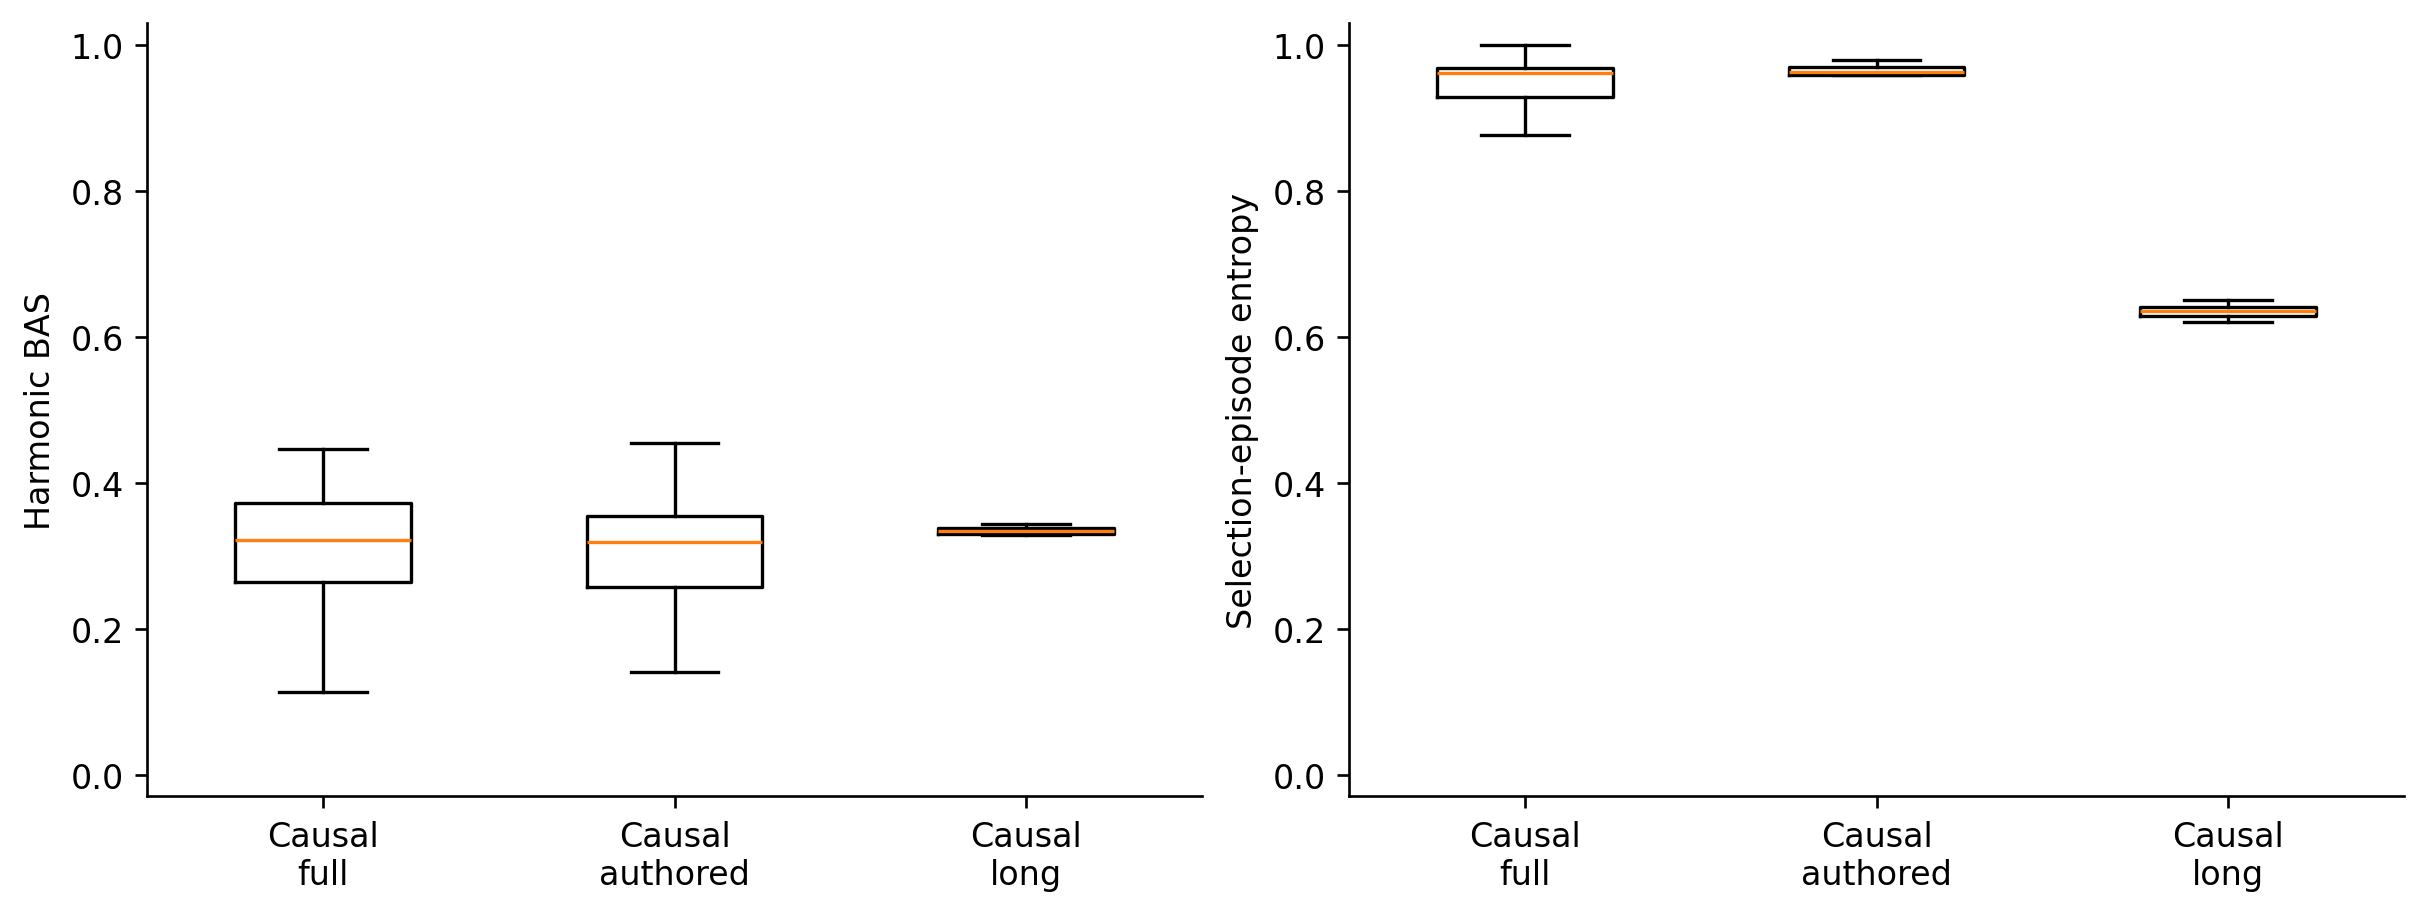
\includegraphics[width=\linewidth]{figures/chapter6_rhythm_diversity.png}
\caption{Distributions of run-level BAS and selection-episode entropy. }
\label{fig:ch6_rhythm}
\end{figure}

Table~\ref{tab:ch6_rhythm} and Figure~\ref{fig:ch6_rhythm} expose variability
that would be hidden by reporting a single BAS. The valid timing ablation is
full versus authored within the causal short suite: sources, seeds, input lengths
and measurement instruments are matched. Comparing the original replay cohort
with the causal cohort would simultaneously change beat information, output-clock
measurement and safety-audit overhead.

In the matched causal comparison, full-system harmonic BAS is
\ChSixFullBas{}, compared with \ChSixAuthoredBas{} for authored timing.
The full-minus-authored gain is \ChSixBasGain{} with a source-bootstrap 95\%
interval of [\ChSixBasGainLow{}, \ChSixBasGainHigh{}]. The interval includes
zero and the Holm-adjusted permutation $p$-value is \ChSixBasHolm{}. The formal
causal evidence therefore does not establish that beat-synchronised timing
improves BAS relative to authored timing under this delivered-beat metric.

\begin{table}[tb]
\centering\scriptsize
\input{experiment_results/reanalysis_rescue_60_v5/chapter6_tables/features.tex}
\medskip

\input{experiment_results/reanalysis_rescue_60_v5/chapter6_tables/groundtruth_div.tex}
\caption{Reconstructed SMPL feature metrics: mean and standard deviation over
five separate 40-output seed evaluations. Ground-truth Div is supplied as a
reference, not a value to exceed. Raw and standardised feature scales must not
be mixed in comparisons.}
\label{tab:ch6_features}
\end{table}

Table~\ref{tab:ch6_features} is deliberately a within-protocol characterisation,
not a leaderboard comparison. Trace phases and blend factors are interpolated
within unchanged motion/transition segments, while categorical switch boundaries
are handled separately. Reconstruction aligns root translation but cannot recover
every sub-trace boundary or the robot's final yaw, limiting and projection effects.
Short ground-truth motions are cycled, potentially introducing root seams. Finally,
the system retrieves real source motions, whereas an unconstrained generator must
produce its own trajectories. These differences can bias FID and Div, and diversity
is interpreted relative to the reference distribution.

The raw geometric Div is only \ChSixGeomDivRatio{} of the ground-truth value,
indicating a narrower reconstructed geometric feature distribution. More
importantly, some ground-truth geometric dimensions have zero variance. Dividing
output deviations by the implemented $10^{-8}$ standard-deviation floor produces
the extremely large standardised geometric values in Table~\ref{tab:ch6_features}.
Those entries diagnose ill-conditioned normalisation, not a meaningful ranking
of dance quality. They are not used as a primary success criterion. The large
raw kinetic scale and its seed variability must also be read alongside the
cyclic-source and reconstruction limitations, rather than compared directly with
published generation benchmarks.

\begin{figure}[tb]
\centering
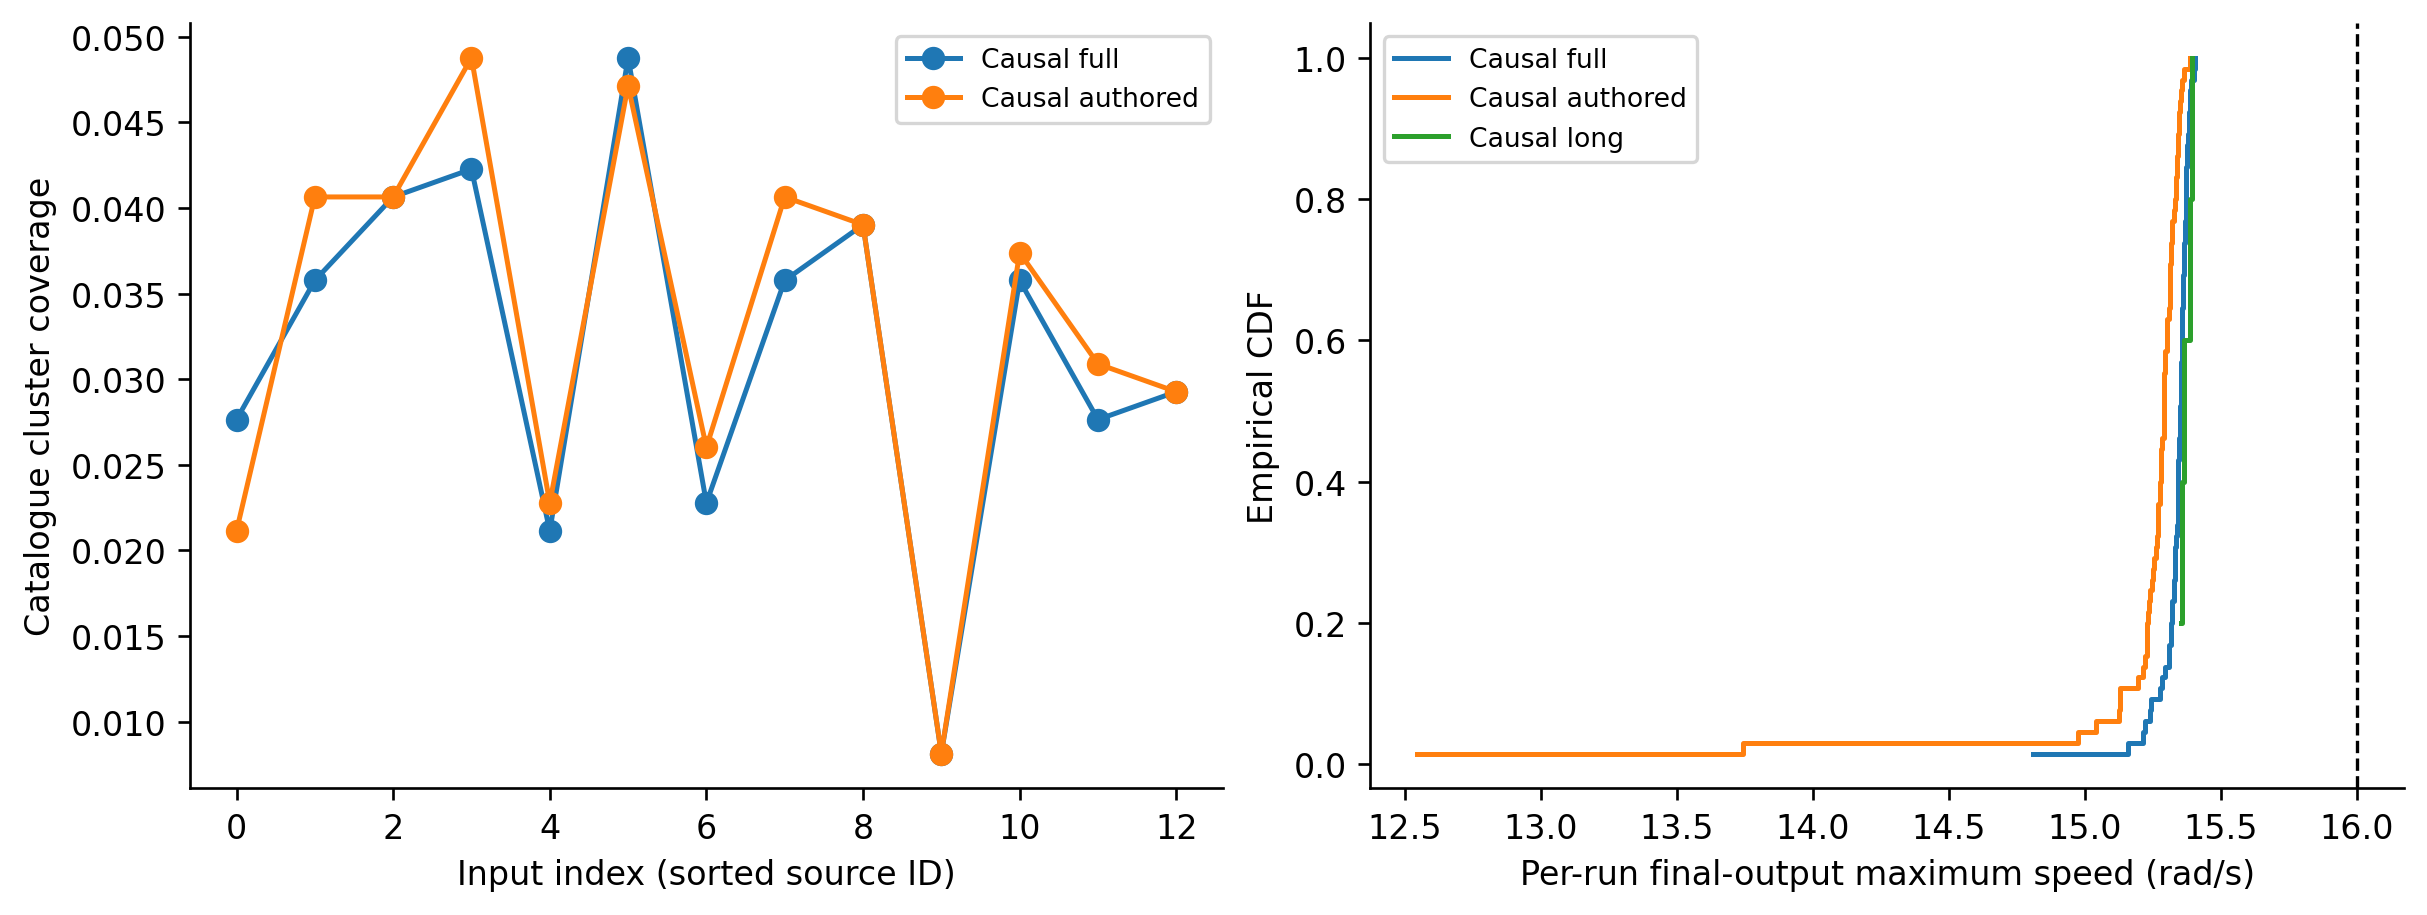
\includegraphics[width=\linewidth]{figures/chapter6_coverage_safety.png}
\caption{Left: mean catalogue-cluster coverage across five seeds per causal
short-suite input, ordered by source ID. Right: empirical distributions of
per-run maximum final-output speed. The dashed line is the 16 rad/s target.
Coverage and command speed measure different aspects of system quality.}
\label{fig:ch6_coverage_safety}
\end{figure}

Coverage complements entropy: an approximately uniform distribution over a small
visited subset is not broad catalogue exploration. Likewise, low adapted PFC
does not establish smooth transitions or balanced locomotion. These measures
jointly qualify the answer to RQ2 instead of reducing dance quality to one score.

\section{Transition Continuity and Safety}

\begin{table}[tb]
\centering\small
\input{experiment_results/reanalysis_rescue_60_v5/chapter6_tables/safety.tex}
\caption{Post-warm-up final-output diagnostics}
\label{tab:ch6_safety}
\end{table}

The causal short full-system peak is \ChSixFullSpeed{} rad/s and the long-run
peak is \ChSixLongSpeed{} rad/s. These are final-output, actual-clock derivatives,
not the limiter's internal nominal-step report. Table~\ref{tab:ch6_safety}
therefore evaluates a stricter and more relevant output contract than checking
the limiter in isolation. The logged position limits, clearance outcomes and
dynamic bounds must each be judged separately.

All 135 causal formal runs pass the registered final-output contract at 60 Hz.
The maximum final speed is 15.4 rad/s in each condition, below the 16 rad/s
limit; the largest acceleration reported in Table~\ref{tab:ch6_safety} is
1673.4 rad/s$^2$, below the 2000 rad/s$^2$ limit. Residual-clearance and final
joint-range violation counts are both zero. Candidate collision detections and
corrective projections still occur, so this result establishes the audited
final-pose contract rather than an absence of interventions.

\begin{figure}[tb]
\centering
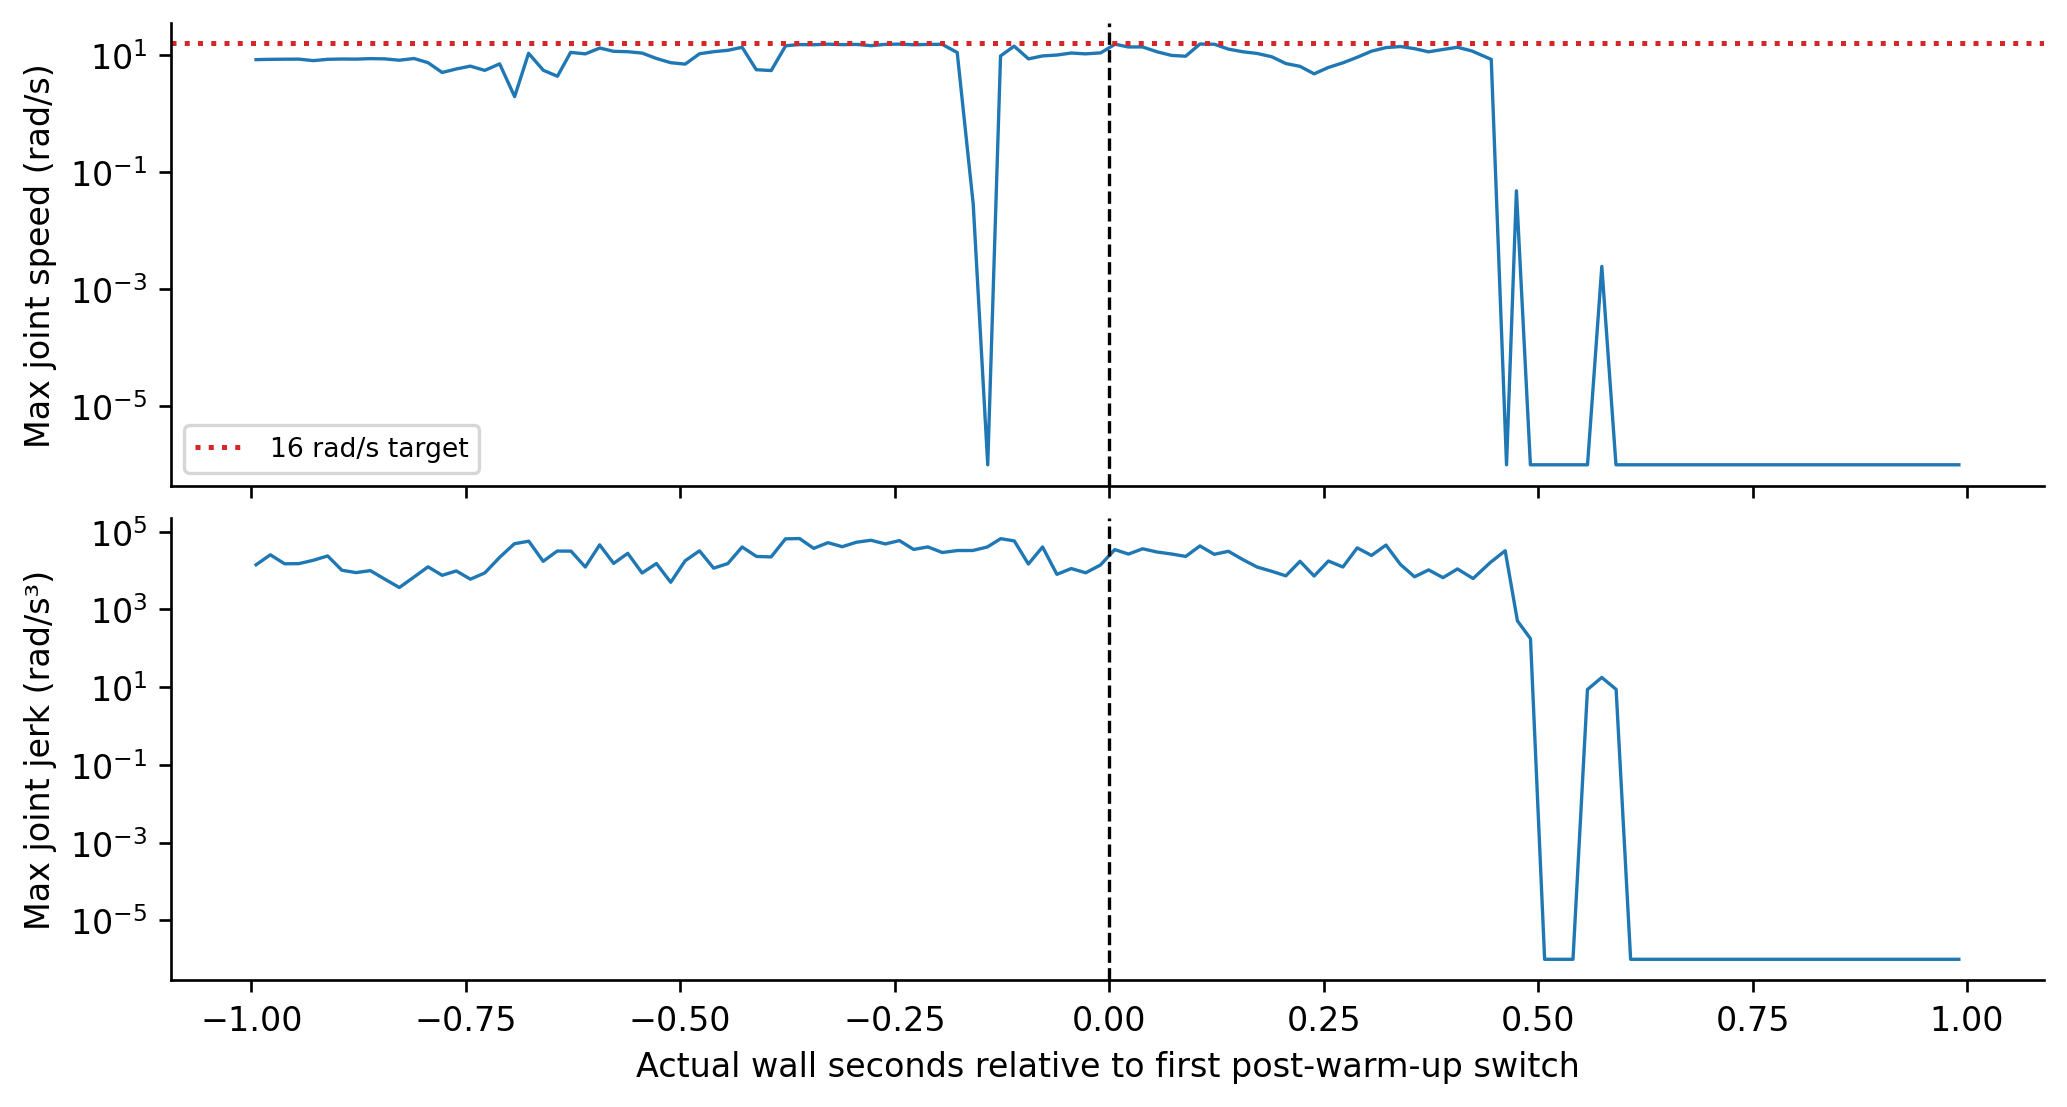
\includegraphics[width=\linewidth]{figures/chapter6_switch_dynamics.png}
\caption{Actual-clock speed and jerk around the first post-warm-up switch in
the fixed causal-full stitched seed-0 run. This is an illustrative trace, not an
average over independent transitions. Logarithmic axes retain large excursions.}
\label{fig:ch6_switch_dynamics}
\end{figure}

The corrected pipeline measures actual output intervals, constrains collision
projection by the remaining dynamic envelope and audits the emitted MuJoCo state.
The formal result supports RQ3 for the registered kinematic bounds at 60 Hz.
It remains a kinematic result: no torque, contact-force, balance or hardware
guarantee follows from these final-pose checks.

\section{Inference Time and End-to-End Response}

\subsection{Computation, preparation and control work}

\begin{table}[tb]
\centering\small
\input{experiment_results/reanalysis_rescue_60_v5/chapter6_tables/timing.tex}
\caption{Medians across runs of each run's query p95, control-work p99 and
deadline-miss ratio. Times are in ms. Failure counts apply the 16.67 ms p99 and
1\% deadline-miss targets to individual runs. These are not pooled frame
percentiles.}
\label{tab:ch6_timing}
\end{table}

\begin{figure}[tb]
\centering
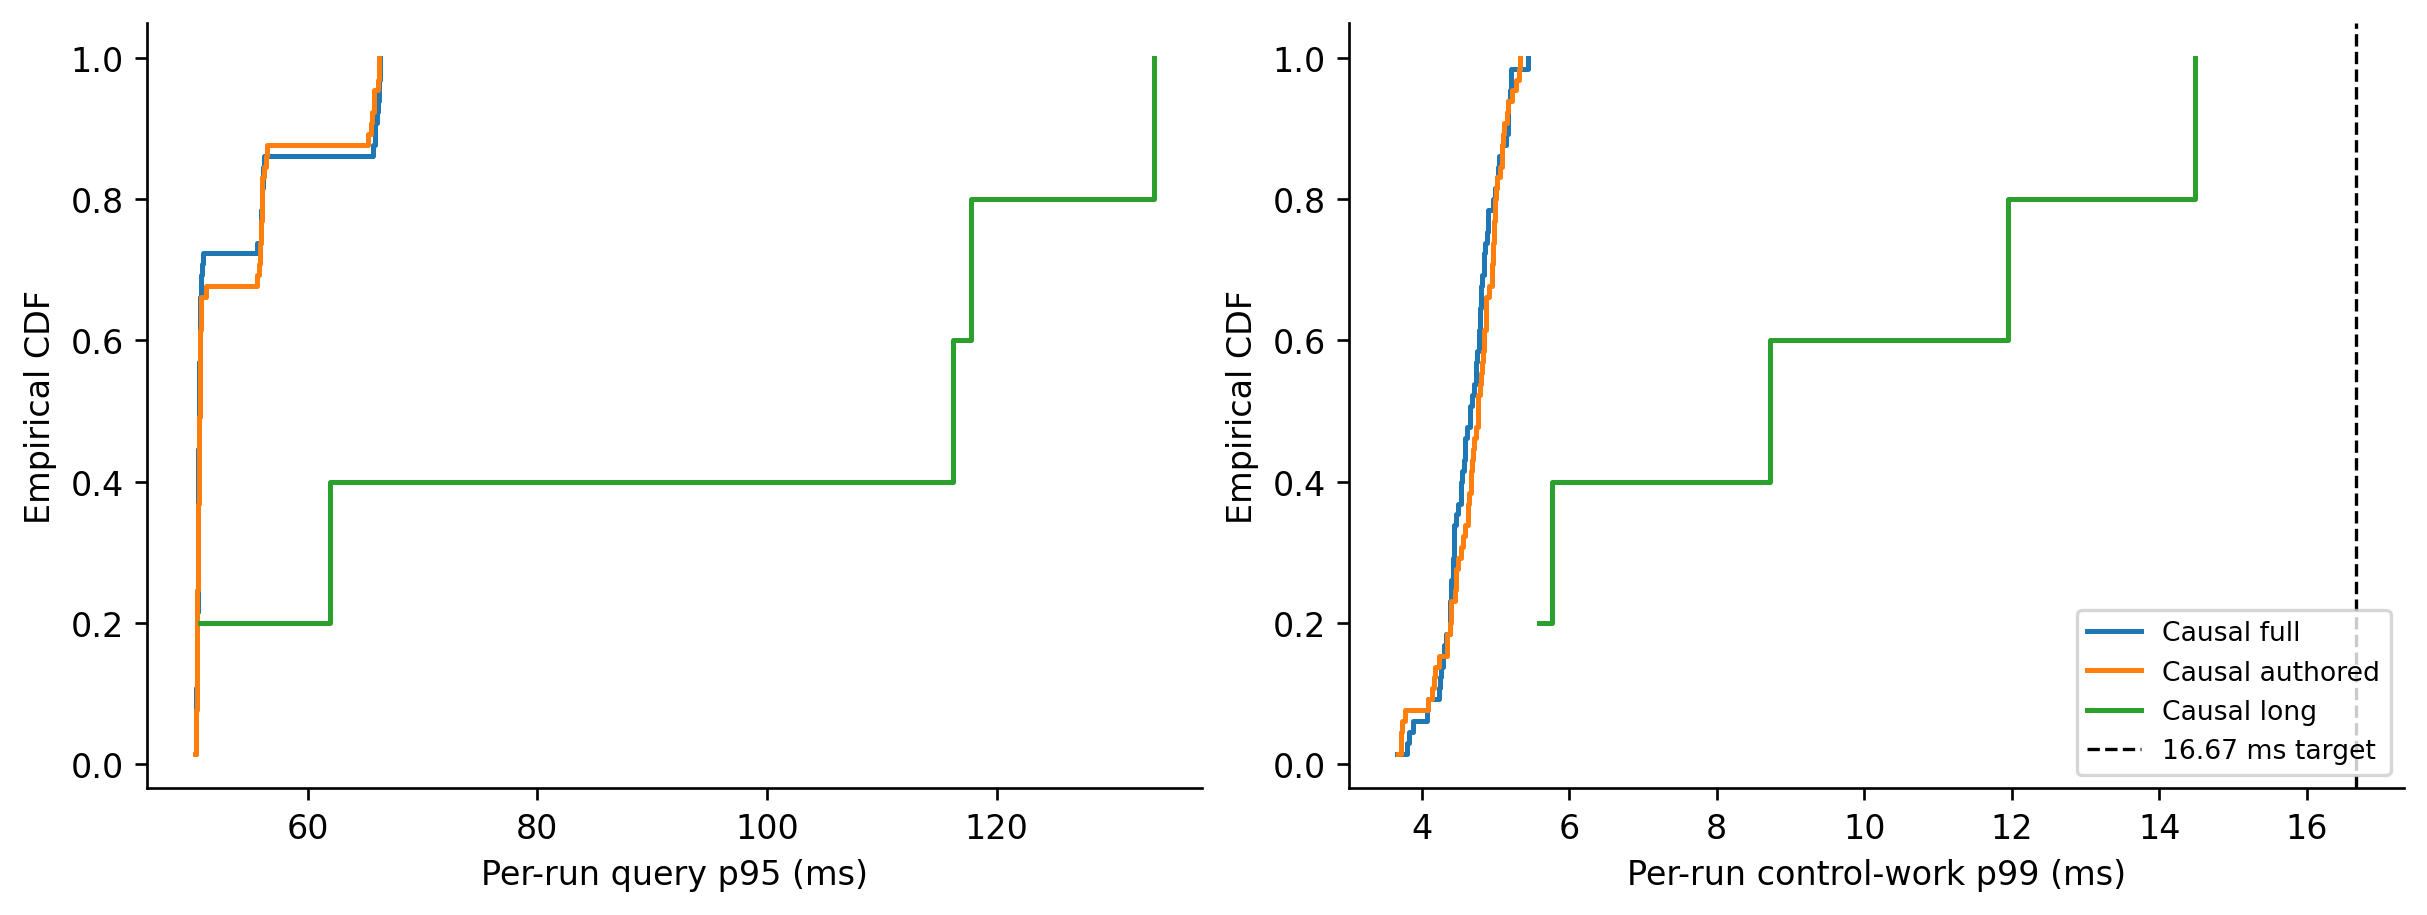
\includegraphics[width=\linewidth]{figures/chapter6_latency_cdf.png}
\caption{Empirical CDFs of per-run latency summaries, not individual query or
frame latencies. The right-hand reference line indicates the nominal 60 Hz
control period.}
\label{fig:ch6_latency}
\end{figure}

The causal short full-system median run-level query p95 is
\ChSixFullQuery{} ms, but its corresponding control-work p99 is
\ChSixFullWork{} ms (Table~\ref{tab:ch6_timing}). Retrieval latency and control
deadline compliance are therefore separate outcomes. The long-run median p99
is \ChSixLongWork{} ms and its median deadline-miss ratio is
\ChSixLongMiss{}. No formal 60 Hz run fails either real-time gate. The worst
individual long run remains below the registered limits, at 14.483 ms p99 and
0.00693 deadline-miss ratio. These are empirical Windows measurements rather
than a hard real-time scheduling guarantee.

\begin{table}[p]
\centering\small
\input{experiment_results/reanalysis_rescue_60_v5/chapter6_tables/stages.tex}
\caption{Stage-resolved timing for the causal full short suite. Each percentile
cell is the median across 65 runs of the within-run percentile, in ms. The last
column is the largest recorded maximum across runs. Nested
stages overlap, asynchronous stages execute concurrently with playback, and
percentiles cannot be added to obtain a total.}
\label{tab:ch6_stages}
\end{table}

\begin{table}[tb]
\centering\small
\input{experiment_results/reanalysis_rescue_60_v5/chapter6_tables/startup.tex}
\caption{Process-start measurements for the causal full short suite. These
startup durations are distinct from steady control work and are not controlled
OS-cache-cold measurements.}
\label{tab:ch6_startup}
\end{table}

Tables~\ref{tab:ch6_stages} and~\ref{tab:ch6_startup} distinguish ONNX execution,
hand-crafted features, track retrieval, motion ranking, candidate preparation
and control work. Candidate grounding and readiness are background operations.
Their wall-clock preparation latency is not an additional synchronous delay on
every control frame. However, asynchronous execution does not remove resource
contention or the need for a candidate to be ready when selected.

\begin{table}[tb]
\centering\small
\input{experiment_results/reanalysis_rescue_60_v5/chapter6_tables/readiness.tex}
\caption{Whole-run operational readiness counters. An underrun means the ready
pool is empty. A hold can occur even when other prepared motions exist. These
counters are not the post-warm-up frame totals used in the safety table.}
\label{tab:ch6_readiness}
\end{table}

The recorded ready-pool underrun and hold-last totals are both zero across all
135 causal formal runs (Table~\ref{tab:ch6_readiness}). The prepared-cache
fallback therefore meets the registered operational readiness targets in this
cohort, although it does not prove readiness for unseen catalogues or platforms.

The supplemental final-output audit performs an additional clearance check,
including forward kinematics. Its overhead is reported separately and remains
inside total control work. Thus differences from the old headless measurements
cannot be attributed solely to causal beat analysis. First-call/cold labels in
some stage counters also do not establish an OS-cache-cold benchmark. Complete
cold/warm distributions for every stage, and a separate mel-construction timer,
are not uniformly available. The chapter reports the timing actually recorded.

Submission attempts require particular care. While a retrieval worker is busy,
the control loop can attempt submission repeatedly before a successful update
advances the matching clock. Consequently, busy attempts divided by all attempts
are not automatically a one-second query-slot loss rate. A completed/submitted
ratio can also include one query still in flight at shutdown. The machine-readable
operational counters are retained, but a 99\% scheduled-slot completion claim is
not established from those counters alone.

\subsection{Musical changes and observable response}

\begin{figure}[tb]
\centering
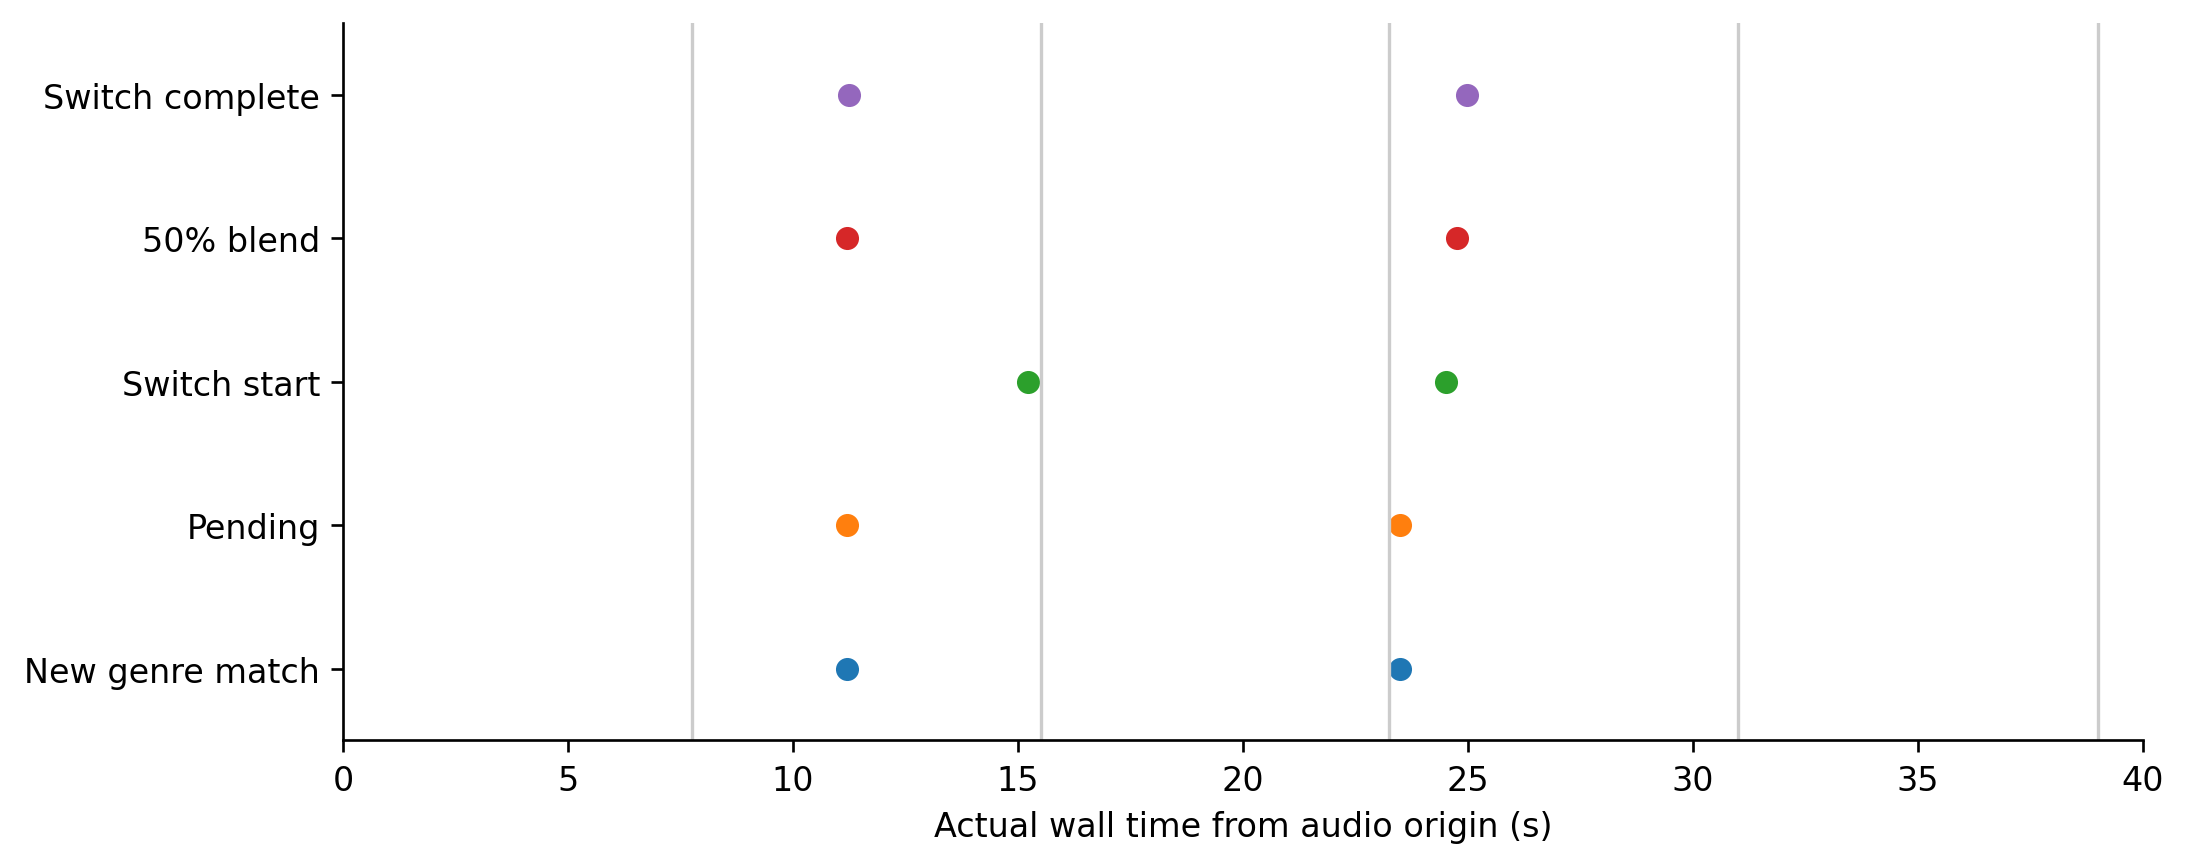
\includegraphics[width=\linewidth]{figures/chapter6_response_timeline.png}
\caption{Deterministically selected illustration: causal full, stitched source,
seed 0. Vertical lines mark source changes. Points mark observed milestones.
Responses are censored at the next change. An absent point is not a zero delay.}
\label{fig:ch6_response}
\end{figure}

Figure~\ref{fig:ch6_response} separates a new genre-compatible ranking from
pending selection, switch initiation, half blending and completion. Six seconds
of accumulated context are needed for the first query, and a post-change window
contains a mixture of old and new audio until that context has been replaced.
Query scheduling, repeated-winner evidence, bar boundaries and candidate readiness
can introduce further waiting. The six-second window is therefore neither an
ONNX inference time nor a universal fixed response latency.

Milestone traces are censored at the next musical change, including the repeated
stitched boundary in long runs. Genre-target matching is available for stitched
inputs. Tempo-jump and silence/recovery milestones are scheduling diagnostics,
not independently verified correct-tempo or correct-rejection responses. Pending
and switch events also need not refer to an identical candidate throughout a
complex change episode. These limitations prevent interpreting every observed
milestone chain as a successful semantic response. RQ4 is answered at the stage
and control-loop level, while fully attributed end-to-end responsiveness remains
a stricter future evaluation requirement.

\section{Ablation Study}

The replay ablations cover legacy retrieval, removal of motion compatibility,
instantaneous top-one selection, removal of bounded-hold diversity, authored
timing, fixed-entry/simple transitions, and disabling the output limiter. The
last condition is restricted to headless diagnostics. Collision checking remains
enabled. The causal supplement retests only the full/authored timing comparison,
not the complete eight-condition matrix.

\begin{table}[tb]
\centering\small
\input{experiment_results/reanalysis_rescue_60_v5/chapter6_tables/ablation.tex}
\caption{Selected paired ablation comparisons after source-level seed averaging.
$\Delta$ is ablation minus full. The Holm family includes all reported
condition-by-metric tests within the relevant suite, not only the selected rows
shown here. Replay jerk is a nominal-rate diagnostic.}
\label{tab:ch6_ablation}
\end{table}

Table~\ref{tab:ch6_ablation} evaluates the registered component hypotheses with
paired tests rather than treating 65 source/seed combinations as independent
music samples. A BAS benefit requires a direction favouring the full system and
support after multiplicity correction. A diversity benefit additionally needs
increased coverage or entropy without more than a 5\% mean relevance loss. A
beat-sync benefit must not increase deadline misses by more than one percentage
point. Absence of significance is not proof of equivalence, but it also does not
justify claiming a component effective because its mean moves in the expected
direction. RQ5 is therefore answered per component and per cohort, rather than by
declaring the entire architecture validated by the existence of an ablation.

In the selected replay comparisons, the apparent directions of retrieval recall,
selection entropy and nominal jerk do not survive Holm correction. In particular,
removing the diversity policy does not produce evidence of lower entropy under
this protocol. The causal authored comparison likewise supplies no corrected
evidence of a BAS difference. Its source-mean deadline-miss ratio differs from
full by \ChSixMissDifference{} (adjusted $p=\ChSixMissHolm{}$), and both
conditions pass the absolute 60 Hz gates. Thus the experiment establishes
neither a BAS benefit nor a deadline penalty for beat synchronisation.
Conditions were executed serially in a fixed matrix order, rather
than randomised across time. Background-load drift remains a possible timing
confound. Here ``causal'' describes audio availability, not a guarantee of
unconfounded causal inference about every performance difference.

\section{Long-Run Reliability}

All five causal long runs completed their registered duration, passed artifact
integrity and passed every evaluated real-time, readiness and final-output gate.
Repeating a 39-second source
for approximately ten minutes stresses recurrent switching and resource use,
but supplies only one source distribution.

The original long-run suite contains eight conditions, each at five seeds. Its
worst result must not be reported as if it belonged to the full system. Likewise,
the original full-system long runs cannot establish causal reliability because
their beat information and instrumentation differ from the supplement. The
causal long runs provide sustained evidence for the selected 60 Hz operating
point. They do not rescue the separate 120 Hz pilot, whose 15/21 failures show
that the original operating target is not reliable on this platform.

\section{Discussion by Research Question}

For RQ1, the leave-one-music-out shortlist provides stronger evidence than the
same-source motion sanity check, but top-one and rejection errors remain material.
For RQ2, rhythm alignment is measurable under a genuinely online delivery protocol,
yet it remains a proxy for musical timing and does not replace judged dance quality.
Coverage, entropy and reference-distribution diversity describe complementary
properties and should not be collapsed into an unrestricted diversity objective.

For RQ3, auditing final qpos verifies the registered end-to-end kinematic
constraints at 60 Hz while preserving the distinction from dynamics and hardware
safety. For RQ4, retrieval computation and asynchronous preparation are explicitly
measurable, and the selected 60 Hz operating point passes the empirical control
gates; the 120 Hz target does not. For RQ5, the paired
statistics delimit the component claims that can be made. Replay ablations and
causal timing ablations answer different experimental questions.

The appropriate overall conclusion is consequently conditional: Humanoid Matcher
is an auditable retrieval and playback pipeline that meets its registered
kinematic and empirical real-time contracts at 60 Hz on the measured platform.
It is not a hard-real-time or physically safe humanoid dance controller, and the
failed 120 Hz capacity test remains an engineering finding rather than evidence
to exclude.

\section{Limitations and Chapter Summary}

The evaluation has no human preference study, no dynamics-based tracking controller
and no hardware trial. BAS, FID/Div, foot-contact proxies and kinematic smoothness
cannot fully assess naturalness, expressiveness or dance aesthetics. The ten CC0
inputs and synthetic negatives provide limited external validity. Five seeds
increase repeatability evidence but do not multiply the number of independent
musical sources.

Further limitations arise from measurement granularity. The original actual
frame clocks cannot be recovered. Low-frequency traces approximate SMPL phase
and transition reconstruction, Cyclic ground truth differs from continuous human
choreography. And query-slot accounting is not identical to repeated submission
attempt accounting. These are stated explicitly rather than hidden behind a
single inference-time or quality number.

This chapter establishes a reproducible record of what the system retrieves,
how its outputs align with delivered beats, where its computation is spent, and
which operating point satisfies the output and timing constraints. Future work
should reduce collision-stage cost if 120 Hz remains a requirement, improve
scheduled-slot and candidate attribution, broaden rejection recordings, and
evaluate closed-loop tracking and human-perceived dance quality. Those extensions
require new evidence. They are not implied by the present kinematic experiments.

% Chapter 7 can be included from a larger thesis with \input or \include.
% Conclusions follow Chapter 6's checksum-verified 60 Hz v5 formal cohort.
% Historical DSP-only, smoke and nominal-clock reports are not pooled with it.

\chapter{Conclusions and Future Work}
\label{chap:conclusions_future_work}

This dissertation investigated how streaming music can guide the selection,
timing and transition of humanoid dance drawn from a finite motion library.
The resulting Humanoid Matcher connects offline AIST++ preparation and G1
retargeting with online music retrieval, stateful motion selection and
continuous kinematic playback. The experiments establish a working,
inspectable integration with measurable rhythm alignment and a validated 60 Hz
operating point, while also identifying an unmet 120 Hz target. This chapter summarises the
work, states the limits of those conclusions and identifies the developments
needed for broader musical coverage and physical robot execution.

\section{Summary of the Work}
\label{sec:ch7_summary}

\paragraph{Data preparation and motion representation.}
The offline pipeline established a traceable association between music,
human choreography and target-robot trajectories. Audio windowing, robust
amplitude normalisation and source-motion analysis produced comparable music
descriptors and velocity-valley key poses. SMPL sequences were converted through
GMR into named-joint, floating-base trajectories for the 29-DoF Unitree G1.
Versioned artefacts, source and model hashes, validated caching and MuJoCo
preflight made catalogue admission explicit. The recorded build contains
411 admitted motions linked to 60 music identities and 348 audio segments.
These checks establish representation and sampled kinematic validity for the
stored clips; they do not certify every subsequent retiming or blend.

\paragraph{Hierarchical music retrieval.}
The final catalogue uses the Discogs EffNet ONNX representation, comprising a
1,280-dimensional embedding and 400 style activations, together with a
24-dimensional DSP rhythm--timbre descriptor. The retargeting artefacts use
pipeline version 4. The DSP-only embedding remains an alternative backend,
requiring a separately built catalogue, rather than the representation evaluated
as the final system. Online queries use six seconds of accumulated audio and
the same extraction and normalisation contract as the reference catalogue.
Segment evidence is pooled at track level, filtered by genre and abstention
rules, and passed to motion ranking. Strict leave-one-music-out evaluation in
Chapter~6 obtained genre Recall@1 of 0.317 and Recall@5 of 0.783. Thus the
representation supplies useful shortlist evidence, although its leading result
is frequently incorrect for unseen music.

\paragraph{Motion compatibility and stable selection.}
The system separates musical similarity from suitability of the associated
movement. Tempo feasibility, key-pose density and motion activity refine the
track-based ranking before selection. Consecutive-winner evidence and a score
margin provide relevance hysteresis, while a bounded-hold policy permits
variation among similarly relevant motions. Prepared-candidate requirements
separate selection intent from execution readiness. These mechanisms make
repetition, rejection and switching decisions observable. Their implementation
is a contribution of the work, but the replay ablations do not establish a
statistically supported benefit for every component after multiplicity
correction; in particular, a diversity benefit cannot be inferred merely from
the presence of a rotation policy.

\paragraph{Beat-aware timing and gradual phase control.}
The timing controller distinguishes detected pulses from events accepted for
motion alignment. Relative beat contrast and authored key-pose spacing guide
beat acceptance, and bounded speed adaptation consumes phase error gradually
instead of resetting the sampler instantaneously. In the matched causal short
suite, harmonic beat alignment score (BAS) was 0.306 under authored timing and
0.313 with the full controller. The source-averaged gain was 0.0067, with a
95\% bootstrap interval of [-0.0078, 0.0228] and a Holm-adjusted $p$-value of
1.0000. The formal experiment therefore does not establish a timing benefit
under the specified delivered-beat metric. Nor does it establish accuracy
against independently annotated musical beats or an improvement in perceived
dance quality.

\paragraph{Continuous switching and output conditioning.}
The transition mechanism searches neighbourhoods of salient target poses using
joint position, velocity, foot-contact, root-state and salience costs. Root
alignment, smoothstep blending, quaternion interpolation and atomic state
transfer connect successive moving trajectories. One-shot completion avoids
an implicit last-to-first seam, while joint limiting and configurable collision
handling condition the output. These mechanisms provide an explicit route from
a selected motion to a displayed pose. The final-output audit verifies that all
135 formal causal runs satisfy the registered joint-range, speed, acceleration
and clearance constraints at 60 Hz. This remains a kinematic contract rather
than evidence of dynamic balance or hardware safety.

\paragraph{Real-time implementation and evaluation.}
Retrieval and candidate preparation execute in bounded background workers,
while the foreground loop consumes completed results and advances playback.
The evaluation records rankings, beat delivery, preparation, transitions,
final poses and actual output clocks. It also separates older preanalysed
file replay from the causal supplement, which contains 130 formal short runs
and five long runs. All 135 pass the registered real-time, readiness and final-
output gates at 60 Hz. A separate 120 Hz pilot passes only 6/21 runs, so the
original frequency is not a reliable operating point on this platform. The
overall achievement is therefore a reproducible retrieval-and-playback system
with an empirically validated 60 Hz configuration and a measured capacity limit.

\section{Limitations}
\label{sec:ch7_limitations}

\paragraph{Kinematic playback and physical feasibility.}
The current player writes root pose and joint positions directly to MuJoCo
state and evaluates forward kinematics. It does not apply a torque-controlled
tracking policy or solve closed-loop balance. Grounding and binary contact
features describe geometric support, without enforcing contact forces, friction,
actuator capacity or disturbance recovery. Consequently, a displayed G1
trajectory may remain dynamically infeasible even when its joint positions and
sampled geometry are valid. No physical Unitree G1 deployment has been evaluated
in this dissertation.

\paragraph{Operating-point and final-output limits.}
The formal 60 Hz cohort passes all registered output constraints: maximum speed
is 15.404 rad/s, maximum acceleration is 1673.415 rad/s$^2$, and both residual
clearance and final joint-range violation counts are zero. Ready-pool underruns
and hold-last events are also zero. These results apply to audited kinematic
poses on the recorded machine. They do not establish torque feasibility,
balance, contact stability or physical-robot safety.

For the causal full short suite, the median run-level control-work p99 is
4.657 ms; the five long runs have a median of 8.724 ms. All 135 formal runs
remain below the 16.67 ms p99 limit and 0.01 deadline-miss-ratio limit, although
the worst long run reaches 14.483 ms and 0.00693 respectively. In contrast, the
separate 120 Hz pilot passes only 6/21 runs: its worst p99 is 15.572 ms against
an 8.33 ms period and its worst miss ratio is 0.18544. The 60 Hz evidence is
therefore empirical soft-real-time evidence for this platform, not a hard-
real-time guarantee or evidence that the original 120 Hz target has been met.

\paragraph{Finite coverage and unequal genre performance.}
The matcher adapts existing clips and cannot supply a movement vocabulary
absent from the catalogue. Its coverage depends on the available AIST++ pairs,
their retargeting quality and manually designed compatibility weights. Musical
similarity is also an indirect proxy for choreographic suitability. Genre
Recall@1 ranged from 1.000 for house to 0.000 for ballet jazz, street jazz and
krump in the six-identities-per-genre evaluation. Broad Discogs-to-AIST++ label
mappings and early genre restriction can propagate a classification error into
the motion candidate set. These results reveal substantial class differences,
while the small number of identities per class limits generalisation.

\paragraph{Metre assumptions and weak-beat behaviour.}
The switch clock groups every four accepted alignment beats into a logical
bar. It does not estimate musical metre or identify downbeats. Since beat
acceptance depends on motion feasibility, rejected subdivisions can also change
the relationship between this clock and the underlying musical pulse. The rule
is therefore poorly suited to triple metre, including waltz, and cannot promise
phrase-aligned switching even for all quadruple-metre music. The observed waltz
retrieval errors should not, however, be attributed to this scheduling rule
without an experiment that isolates metre from retrieval.

For ambient or otherwise weakly rhythmic input, persistent negative-style and
beat-quality gates provide conservative abstention. The ambient CC0 recording
was rejected in 96\% of evaluated windows, but one recording is insufficient
evidence of robust handling of the category. Holding the active motion or
returning towards authored timing can remain musically inappropriate when the
audio becomes quiet or loses its pulse. In particular, reducing secondary pose
modulation does not necessarily stop the underlying authored trajectory. The
system lacks a fully specified transition from dancing to low-activity behaviour
and back, calibrated across diverse weak-beat recordings.

\paragraph{Engineering proxies and experimental coverage.}
No user study assesses naturalness, expressiveness or preference. BAS measures
alignment to delivered detector events, while contact proxies, entropy,
coverage and smoothness each capture only part of dance quality. Reconstructed
SMPL FID/Div additionally depend on trace interpolation, source-motion reuse
and cyclic reference construction. Near-zero reference variance makes some
standardised geometric results ill-conditioned, so they cannot support an
aesthetic ranking. The ten external CC0 recordings and synthetic negatives
offer limited acoustic diversity; headless file-input trials do not reproduce
microphone reverberation, clipping or room noise. Repeated seeds improve
repeatability evidence without creating independent musical sources, and the
causal long runs repeat only one stitched source. The causal supplement also
retests only full versus authored timing, so the complete replay ablation matrix
cannot be treated as causal online validation.

\section{Future Work}
\label{sec:ch7_future_work}

\paragraph{Extend the validated operating envelope.}
The immediate systems priority is to preserve the coherent final-output contract
while reducing foreground work enough to evaluate 120 Hz again. A short-horizon
constrained trajectory update could incorporate collision correction within the
same temporal problem as joint limiting. Its feasibility and fallback behaviour
should continue to be evaluated from actual output timestamps rather than from
an intermediate limiter report. Profiling should guide reductions in repeated
grounding work and especially foreground collision cost, with prepared data
reused under an explicit model-and-version contract. New comparisons should
freeze the machine, backend,
window settings and audit configuration, and counterbalance run order to reduce
background-load confounding. Explicit query-slot identifiers and a persistent
candidate identifier across match, pending, readiness and blend events would
also make end-to-end response attribution more reliable.

\paragraph{Metre and downbeat-aware control.}
A causal beat, downbeat and metre estimator could replace the fixed four-event
clock with an estimate of musical position. The scheduler should distinguish
the underlying beat sequence from the subset used for motion alignment, so
skipping an infeasible accent does not redefine the bar. Uncertain metre should
lead to a documented beat-level fallback rather than an assumed downbeat.
Evaluation should include triple metre, compound metre, tempo changes and weak
percussion, using independently annotated beat and downbeat times alongside
detector delivery latency. A complementary phase study should cover at least
three distinct motions per genre, stratified by tempo and key-pose density;
multiple windows or seeds of one motion should not count as additional motions.

\paragraph{Learned transition-entry scoring.}
The current weighted entry cost offers a useful baseline for learning which
candidate state produces a successful transition. Training examples could
combine current and target pose, velocity, contact, root motion and musical
context with measured transition outcomes and human pairwise preferences.
A learned ranker could then capture interactions that a fixed weighted sum
misses, while explicit feasibility checks continue to determine admissibility.
Evaluation should hold out source motions and music identities and compare the
ranker with the existing cost on both perceived continuity and final-output
constraints. An improved prediction score alone would not establish a better
executed transition.

\paragraph{Motion-fragment retrieval and composition.}
The existing system can enter partway through a selected clip, but retrieval
and activity metadata remain primarily clip-level. A fragment catalogue could
instead index phrases or contact-consistent movement units, each with local
music descriptors, entry and exit states, duration and feasible tempo range.
Searching compatible fragment sequences would permit finer responses to changes
within a song and reuse a larger combination of existing motifs. A sparse
transition graph or bounded-horizon search could balance music relevance,
contact compatibility and motif continuity. Such an extension needs new checks
for the joins and composed sequence: validating each fragment separately would
not establish that their concatenation is feasible. Diversity should remain
subordinate to coherent phrasing rather than encourage rapid switching.

\paragraph{Contact-constrained tracking and balance.}
Foot-contact states should become constraints on execution rather than only
terms in entry ranking. A subsequent controller could combine support-phase
information, foot placement and floating-base state estimation with whole-body
inverse dynamics, model-predictive control or a learned tracking policy. Its
role would be to track the selected reference subject to contact and actuator
constraints, reducing motion intensity or delaying a transition when necessary.
Dynamics-based simulation should evaluate tracking error, foot slip, support
transitions, torque saturation and recovery from disturbances. This would test
a different and stronger claim than the present kinematic preview.

\paragraph{Physical Unitree G1 deployment.}
Hardware integration should follow validated closed-loop simulation and a
measured final-output contract. The music matcher would supply motion references
to the tracking controller rather than directly assign the physical root state.
Initial trials could progress from supported, low-amplitude movements to
freestanding sequences and then music-driven transitions. They should record
microphone acquisition, communication and actuator-response delays separately,
as well as tracking failures and interventions. This staged evaluation would
reveal how acoustic conditions, state-estimation error and actuator limits
change the behaviour observed in headless file-input experiments.

\paragraph{User preference and weak-beat adaptation.}
A preference-aware selector could allow users to favour particular styles,
energy levels or degrees of repetition within the feasible candidate set.
Pairwise judgements of musical fit, transition naturalness and overall appeal
would support both preference learning and a direct evaluation of dance quality.
Weak-beat behaviour should similarly become a selectable, explicit response:
for example, a controlled change to a low-activity motion followed by a gradual
return when rhythmic evidence recovers. Additional real ambient, speech, noise
and mixed recordings are needed to calibrate rejection and recovery separately.
User preferences should influence the choice among feasible motions while
preserving execution constraints, and subjective gains should be reported
alongside relevance, continuity and timing measurements.

The work provides a basis for these extensions by making the chain from musical
evidence to robot pose traceable. Its current results support finite-library
retrieval and a 60 Hz kinematic operating point, but do not establish that causal
phase control improves BAS or that 120 Hz is reliable. They demonstrate why
musical responsiveness, output feasibility and real-time compliance must be
evaluated separately. Resolving their interaction is the next step towards a
humanoid that can perform continuously and expressively under physical control.



   


\bibliographystyle{plain}
\bibliography{references}

\appendix

% Include after \appendix in the parent thesis with
% % Include after \appendix in the parent thesis with
% % Include after \appendix in the parent thesis with
% \input{appendix_source_code} or \include{appendix_source_code}.
% The parent thesis should load the hyperref package for clickable URLs.

\chapter{Source Code Repository}
\label{app:source_code}

The source code for the BeatWeaver system described in this dissertation is
available in the following GitHub repository:

\begin{center}
    \url{https://github.com/EddieOuyang2004/MusicRobot/tree/main}
\end{center}

The humanoid implementation is located in
\texttt{realtime/humanoid\_robot/}. Readers should consult the repository's
top-level README and the README in that directory for the project structure
and instructions for running the system.
 or % Include after \appendix in the parent thesis with
% \input{appendix_source_code} or \include{appendix_source_code}.
% The parent thesis should load the hyperref package for clickable URLs.

\chapter{Source Code Repository}
\label{app:source_code}

The source code for the BeatWeaver system described in this dissertation is
available in the following GitHub repository:

\begin{center}
    \url{https://github.com/EddieOuyang2004/MusicRobot/tree/main}
\end{center}

The humanoid implementation is located in
\texttt{realtime/humanoid\_robot/}. Readers should consult the repository's
top-level README and the README in that directory for the project structure
and instructions for running the system.
.
% The parent thesis should load the hyperref package for clickable URLs.

\chapter{Source Code Repository}
\label{app:source_code}

The source code for the BeatWeaver system described in this dissertation is
available in the following GitHub repository:

\begin{center}
    \url{https://github.com/EddieOuyang2004/MusicRobot/tree/main}
\end{center}

The humanoid implementation is located in
\texttt{realtime/humanoid\_robot/}. Readers should consult the repository's
top-level README and the README in that directory for the project structure
and instructions for running the system.
 or % Include after \appendix in the parent thesis with
% % Include after \appendix in the parent thesis with
% \input{appendix_source_code} or \include{appendix_source_code}.
% The parent thesis should load the hyperref package for clickable URLs.

\chapter{Source Code Repository}
\label{app:source_code}

The source code for the BeatWeaver system described in this dissertation is
available in the following GitHub repository:

\begin{center}
    \url{https://github.com/EddieOuyang2004/MusicRobot/tree/main}
\end{center}

The humanoid implementation is located in
\texttt{realtime/humanoid\_robot/}. Readers should consult the repository's
top-level README and the README in that directory for the project structure
and instructions for running the system.
 or % Include after \appendix in the parent thesis with
% \input{appendix_source_code} or \include{appendix_source_code}.
% The parent thesis should load the hyperref package for clickable URLs.

\chapter{Source Code Repository}
\label{app:source_code}

The source code for the BeatWeaver system described in this dissertation is
available in the following GitHub repository:

\begin{center}
    \url{https://github.com/EddieOuyang2004/MusicRobot/tree/main}
\end{center}

The humanoid implementation is located in
\texttt{realtime/humanoid\_robot/}. Readers should consult the repository's
top-level README and the README in that directory for the project structure
and instructions for running the system.
.
% The parent thesis should load the hyperref package for clickable URLs.

\chapter{Source Code Repository}
\label{app:source_code}

The source code for the BeatWeaver system described in this dissertation is
available in the following GitHub repository:

\begin{center}
    \url{https://github.com/EddieOuyang2004/MusicRobot/tree/main}
\end{center}

The humanoid implementation is located in
\texttt{realtime/humanoid\_robot/}. Readers should consult the repository's
top-level README and the README in that directory for the project structure
and instructions for running the system.
.
% The parent thesis should load the hyperref package for clickable URLs.

\chapter{Source Code Repository}
\label{app:source_code}

The source code for the BeatWeaver system described in this dissertation is
available in the following GitHub repository:

\begin{center}
    \url{https://github.com/EddieOuyang2004/MusicRobot/tree/main}
\end{center}

The humanoid implementation is located in
\texttt{realtime/humanoid\_robot/}. Readers should consult the repository's
top-level README and the README in that directory for the project structure
and instructions for running the system.


\end{document}
